\documentclass[11pt,a4paper,openany]{report}

% --- Page Geometry ---
\usepackage[a4paper, top=2.6cm, bottom=2.5cm, left=2.3cm, right=2.3cm, headheight=22pt]{geometry}

% --- Fonts & Typography ---
\usepackage[utf8]{inputenc}
\usepackage[T1]{fontenc}
\usepackage{lmodern}
\usepackage{microtype}

% --- Mathematics Packages ---
\usepackage{amsmath,amssymb,amsfonts,amsthm,mathtools}
\usepackage{bm}
\usepackage{enumitem}

% --- Neutralize LaTeX 2026 Table Tagging Socket in Framed Boxes ---
\ExplSyntaxOn
\cs_gset_eq:NN \__tbl_tag_cell_end: \prg_do_nothing:
\cs_gset_eq:NN \__tbl_tag_row_end: \prg_do_nothing:
\ExplSyntaxOff

% --- Colors ---
\usepackage[dvipsnames,svgnames,x11names]{xcolor}
\definecolor{primary}{RGB}{18, 48, 86}      % Deep Navy
\definecolor{secondary}{RGB}{0, 119, 137}   % Ocean Teal
\definecolor{accent}{RGB}{194, 65, 12}      % Warm Amber/Rust
\definecolor{success}{RGB}{22, 101, 52}     % Emerald Forest
\definecolor{boxbg}{RGB}{248, 250, 252}     % Slate Tint Light
\definecolor{rulecolor}{RGB}{203, 213, 225} % Slate Border

% --- TikZ Graphics ---
\usepackage{tikz}
\usetikzlibrary{calc,angles,quotes,3d,perspective,arrows.meta,decorations.pathreplacing,decorations.markings,shapes.geometric,patterns}

% --- Beautiful Framed Environments with mdframed ---
\usepackage{mdframed}

\newcommand{\tcblower}{\par\vspace{0.5em}\noindent{\color{black!15}\hrule height 0.8pt}\vspace{0.6em}}

\mdfdefinestyle{conceptstyle}{
    backgroundcolor=secondary!3!white,
    linecolor=secondary!60,
    linewidth=0.9pt,
    roundcorner=5pt,
    innertopmargin=8pt,
    innerbottommargin=8pt,
    innerleftmargin=12pt,
    innerrightmargin=12pt,
    frametitleaboveskip=5pt,
    frametitlebelowskip=5pt,
    frametitlerule=true,
    frametitlerulewidth=0.5pt,
    frametitlerulecolor=secondary!20,
    nobreak=true
}

\mdfdefinestyle{theoremstyle}{
    backgroundcolor=primary!3!white,
    linecolor=primary!65,
    linewidth=0.9pt,
    roundcorner=5pt,
    innertopmargin=8pt,
    innerbottommargin=8pt,
    innerleftmargin=12pt,
    innerrightmargin=12pt,
    frametitleaboveskip=5pt,
    frametitlerule=true,
    frametitlerulewidth=0.5pt,
    frametitlerulecolor=primary!20,
    frametitlebelowskip=5pt,
    nobreak=true
}

\mdfdefinestyle{examplestyle}{
    backgroundcolor=success!3!white,
    linecolor=success!60,
    linewidth=0.9pt,
    roundcorner=5pt,
    innertopmargin=8pt,
    innerbottommargin=8pt,
    innerleftmargin=12pt,
    innerrightmargin=12pt,
    frametitleaboveskip=5pt,
    frametitlebelowskip=5pt,
    frametitlerule=true,
    frametitlerulewidth=0.5pt,
    frametitlerulecolor=success!20,
    nobreak=true
}

\mdfdefinestyle{notestyle}{
    backgroundcolor=accent!4!white,
    linecolor=accent!60,
    linewidth=0.9pt,
    roundcorner=5pt,
    innertopmargin=8pt,
    innerbottommargin=8pt,
    innerleftmargin=12pt,
    innerrightmargin=12pt,
    frametitleaboveskip=5pt,
    frametitlebelowskip=5pt,
    frametitlerule=true,
    frametitlerulewidth=0.5pt,
    frametitlerulecolor=accent!20,
    nobreak=true
}

\newenvironment{conceptbox}[1][]{
    \ifstrempty{#1}{%
        \begin{mdframed}[style=conceptstyle, frametitlerule=false]%
    }{%
        \begin{mdframed}[style=conceptstyle, frametitle={\textbf{\color{secondary}#1}}]%
    }%
}{\end{mdframed}}

\newenvironment{theorembox}[1][]{
    \ifstrempty{#1}{%
        \begin{mdframed}[style=theoremstyle, frametitlerule=false]%
    }{%
        \begin{mdframed}[style=theoremstyle, frametitle={\textbf{\color{primary}#1}}]%
    }%
}{\end{mdframed}}

\newenvironment{examplebox}[1][]{
    \ifstrempty{#1}{%
        \begin{mdframed}[style=examplestyle, frametitlerule=false]%
    }{%
        \begin{mdframed}[style=examplestyle, frametitle={\textbf{\color{success}#1}}]%
    }%
}{\end{mdframed}}

\newenvironment{notebox}[1][Note \& Analysis]{
    \ifstrempty{#1}{%
        \begin{mdframed}[style=notestyle, frametitlerule=false]%
    }{%
        \begin{mdframed}[style=notestyle, frametitle={\textbf{\color{accent}#1}}]%
    }%
}{\end{mdframed}}

% --- Headers & Footers ---
\usepackage{fancyhdr}
\pagestyle{fancy}
\fancyhf{}
\fancyhead[L]{\small\color{primary!80}\nouppercase{\leftmark}}
\fancyhead[R]{\small\bfseries\color{primary}\thepage}
\fancyfoot[L]{\scriptsize\color{gray!75}Numerical Analysis --- \href{https://sciqb.com}{\color{secondary}\textbf{sciqb}}}
\fancyfoot[R]{\scriptsize\color{gray!75}Comprehensive Lecture Notes}
\renewcommand{\headrulewidth}{0.5pt}
\renewcommand{\headrule}{\hbox to\headwidth{\color{primary!25}\leaders\hrule height \headrulewidth\hfill}}
\renewcommand{\footrulewidth}{0.3pt}
\renewcommand{\footrule}{\hbox to\headwidth{\color{gray!20}\leaders\hrule height \footrulewidth\hfill}}

\fancypagestyle{plain}{%
  \fancyhf{}%
  \fancyfoot[L]{\scriptsize\color{gray!75}Numerical Analysis --- \href{https://sciqb.com}{\color{secondary}\textbf{sciqb}}}%
  \fancyfoot[R]{\scriptsize\bfseries\color{primary}\thepage}%
  \renewcommand{\headrulewidth}{0pt}%
  \renewcommand{\footrulewidth}{0.3pt}%
  \renewcommand{\footrule}{\hbox to\headwidth{\color{gray!20}\leaders\hrule height \footrulewidth\hfill}}%
}

% --- Section Styling ---
\usepackage{titlesec}
\titleformat{\chapter}[display]
  {\normalfont\bfseries\color{primary}}
  {\small\bfseries\color{secondary}\MakeUppercase{\chaptertitlename}\ \Huge\thechapter}
  {4pt}
  {\Huge\bfseries}
  [\vspace{4pt}{\color{secondary!40}\hrule height 1.2pt}]
\titleformat{\section}
  {\normalfont\Large\bfseries\color{primary}}{\thesection}{1em}{}
\titleformat{\subsection}
  {\normalfont\large\bfseries\color{secondary}}{\thesubsection}{1em}{}

% --- Hyperref & PDF Metadata ---
\usepackage[bookmarks=true,bookmarksnumbered=true,colorlinks=true,
  linkcolor=primary,citecolor=secondary,urlcolor=accent]{hyperref}
\hypersetup{
  pdftitle={Numerical Analysis by sciqb},
  pdfauthor={sciqb},
  pdfsubject={Numerical Analysis Comprehensive Lecture Notes (Pages 1--68)},
  pdfcreator={sciqb.com}
}

% --- Document Metadata ---
\title{\Huge\textbf{\color{primary}Numerical Analysis}\\[0.35cm]
\LARGE\textbf{\color{secondary}by \href{https://sciqb.com}{\color{secondary}\underline{sciqb}}}\\[0.45cm]
\Large\textbf{\color{secondary!85}Complete Lecture Notes, Rigorous Derivations, TikZ Geometric Diagrams, Algorithm Proofs, and Solved Examination Problems}\\[0.2cm]
\normalsize\textit{Transcribed and Enhanced Page-by-Page from Manuscript (Pages 1--68)}}
\author{\textbf{\Large \href{https://sciqb.com}{sciqb}}\\[0.15cm]\small\href{https://sciqb.com}{\color{secondary}https://sciqb.com}}
\date{\large Academic Session 2026}

\begin{document}

\maketitle

\begin{abstract}
\noindent This compendium presents a definitive, rigorous, and visually enriched textbook of \textbf{Numerical Analysis}, faithfully capturing the entire 68-page curriculum of university lecture notes. Topics encompass the numerical solution of nonlinear algebraic and transcendental equations (Secant method, Regula-Falsi method, Newton-Raphson method, fixed-point iterations, order of convergence derivations, multipoint acceleration), direct and iterative solutions of linear systems (Gauss elimination with partial pivoting, Gauss-Jordan, Jacobi and Gauss-Seidel iterations, matrix splittings), eigenvalues and matrix bounds (Gerschgorin circle theorem and complete proof, Power method for dominant eigenvalues), the calculus of finite differences and operational identities ($\Delta, \nabla, E, \delta, \mu, D$ operator algebras, factorial polynomials, series summation), interpolation theory for equal and unequal intervals (Newton forward and backward difference formulas, Lagrange interpolation, divided difference calculus, Newton's divided difference formula), and numerical quadrature (general Newton-Cotes formula, Trapezoidal rule, Simpson's 1/3 and 3/8 rules, Weddle's rule, and asymptotic truncation error analysis). Every theorem is proven with exhaustive algebraic detail, supported by high-precision TikZ vector graphics and step-by-step arithmetic verification.
\end{abstract}

\vspace{1cm}
\tableofcontents
\newpage

% --- Chapter Inclusions (Pages 1--68) ---
\chapter{Numerical Solution of Algebraic and Transcendental Equations (Pages 1--23)}
\label{ch:root_finding}

\begin{conceptbox}[Foundational Principles of Nonlinear Root-Finding]
A fundamental problem in numerical analysis is determining the root $\alpha \in \mathbb{R}$ of a nonlinear equation:
\begin{equation}
    f(x) = 0
\end{equation}
where $f(x)$ is an algebraic polynomial or transcendental function (involving trigonometric, exponential, or logarithmic terms). In general, closed-form analytic solutions do not exist for polynomials of degree $n \ge 5$ (Abel--Ruffini theorem) or for transcendental equations. Consequently, iterative numerical algorithms are essential.

An iterative method generates a sequence of approximations $\{x_k\}_{k=0}^\infty$ from one or more initial guesses that converges asymptotically to the true root $\alpha$:
\begin{equation}
    \lim_{k \to \infty} x_k = \alpha
\end{equation}
The effectiveness of an iterative method is governed by its \textbf{order of convergence}, computational cost per iteration (function and derivative evaluations), and \textbf{basin of convergence}.
\end{conceptbox}

% =========================================================================
% PAGE 1: SECANT METHOD
% =========================================================================
\section{Page 1: The Secant Method --- Geometric Derivation and Formulation}
\label{sec:page1_secant}

\begin{theorembox}[Geometric Derivation of the Secant Iteration Formula]
Let $f(x) = 0$ possess a continuous real root in $[a, b]$. In the Secant method, we do not require the derivative $f'(x)$. Instead, we select two initial approximations:
\begin{equation}
    x_0 = a, \quad x_1 = b
\end{equation}
Consider the two points on the curve $y = f(x)$:
\begin{equation}
    A\big(x_0, f(x_0)\big) \quad \text{and} \quad B\big(x_1, f(x_1)\big)
\end{equation}
The secant line (chord) connecting $A$ and $B$ has the two-point Cartesian equation:
\begin{equation}
    y - f(x_1) = \frac{f(x_1) - f(x_0)}{x_1 - x_0}(x - x_1)
\end{equation}
The next approximation $x_2$ is defined as the $x$-intercept of this secant line (setting $y = 0$):
\begin{equation}
    0 - f(x_1) = \frac{f(x_1) - f(x_0)}{x_1 - x_0}(x_2 - x_1)
\end{equation}
Solving for $x_2$:
\begin{equation}
    \boxed{x_2 = x_1 - \frac{x_1 - x_0}{f(x_1) - f(x_0)} f(x_1)}
\end{equation}
Repeating this process through the points $\big(x_1, f(x_1)\big)$ and $\big(x_2, f(x_2)\big)$, the subsequent root estimate $x_3$ is:
\begin{equation}
    x_3 = x_2 - \frac{x_2 - x_1}{f(x_2) - f(x_1)} f(x_2)
\end{equation}
By mathematical induction, the general $(k+1)$-th Secant iteration formula is:
\begin{equation}
    \boxed{x_{k+1} = x_k - \frac{x_k - x_{k-1}}{f(x_k) - f(x_{k-1})} f(x_k) = \frac{x_{k-1}f(x_k) - x_k f(x_{k-1})}{f(x_k) - f(x_{k-1})}} \quad (k = 1, 2, 3, \dots)
\end{equation}
\end{theorembox}

\begin{center}
\begin{tikzpicture}[scale=1.15]
    % Axes
    \draw[->, thick, primary] (-0.5, 0) -- (6.5, 0) node[right, primary] {$x$};
    \draw[->, thick, primary] (0, -2.5) -- (0, 3.5) node[above, primary] {$y$};
    
    % Curve f(x)
    \draw[very thick, secondary, domain=0.8:5.5, samples=100] 
        plot (\x, {0.25*(\x-1.5)*(\x-1.5)*(\x-1.5) - 0.7}) 
        node[right] {$y = f(x)$};
    
    % Exact root alpha
    \coordinate (Alpha) at (3.154, 0);
    \filldraw[accent] (Alpha) circle (2pt) node[below=4pt, accent] {$\alpha$ (Exact Root)};
    
    % Points x0 and x1
    \coordinate (X0) at (1.2, 0);
    \coordinate (FX0) at (1.2, -0.7067);
    \coordinate (X1) at (5.0, 0);
    \coordinate (FX1) at (5.0, 2.372);
    
    % Secant line 1 through (x0, f(x0)) and (x1, f(x1))
    \draw[thick, ForestGreen, dashed] (1.0, -0.869) -- (5.2, 2.534);
    
    % Intersection x2
    \coordinate (X2) at (2.072, 0);
    \coordinate (FX2) at (2.072, -0.653);
    
    % Secant line 2 through (x1, f(x1)) and (x2, f(x2))
    \draw[thick, DarkOrange, dashed] (1.8, -0.934) -- (5.2, 2.579);
    \coordinate (X3) at (2.703, 0);
    
    % Drop lines
    \draw[dotted, gray] (X0) -- (FX0);
    \draw[dotted, gray] (X1) -- (FX1);
    \draw[dotted, gray] (X2) -- (FX2);
    
    % Dots and labels
    \filldraw[ForestGreen] (FX0) circle (2pt) node[left=2pt] {$A\big(x_0, f(x_0)\big)$};
    \filldraw[ForestGreen] (FX1) circle (2pt) node[above left=2pt] {$B\big(x_1, f(x_1)\big)$};
    \filldraw[DarkOrange] (FX2) circle (2pt) node[right=3pt] {$C\big(x_2, f(x_2)\big)$};
    
    \filldraw[primary] (X0) circle (1.5pt) node[above=2pt] {$x_0$};
    \filldraw[primary] (X1) circle (1.5pt) node[below=2pt] {$x_1$};
    \filldraw[ForestGreen] (X2) circle (1.8pt) node[below=2pt, ForestGreen] {$x_2$};
    \filldraw[DarkOrange] (X3) circle (1.8pt) node[below=2pt, DarkOrange] {$x_3$};
\end{tikzpicture}
\end{center}

\begin{examplebox}[Manuscript Problem: Locating Root for $x^3 + x^2 - 1 = 0$]
\textbf{Problem Statement (Manuscript Page 1):}
Find the real root of the cubic equation:
\begin{equation}
    f(x) \equiv x^3 + x^2 - 1 = 0
\end{equation}
\textbf{Initial Root Bracketing:}
We evaluate $f(x)$ at convenient integer points:
\begin{align}
    f(0) &= 0^3 + 0^2 - 1 = -1 < 0 \\
    f(1) &= 1^3 + 1^2 - 1 = +1 > 0
\end{align}
By the Intermediate Value Theorem, since $f(0) \cdot f(1) < 0$, at least one real root lies in the interval:
\begin{equation}
    [a, b] = [0, 1] \implies x_0 = 0, \quad x_1 = 1
\end{equation}
\end{examplebox}

% =========================================================================
% PAGE 2: REGULA-FALSI COMPARISON
% =========================================================================
\section{Page 2: Regula-Falsi (False Position) Method and Comparative Iterations}
\label{sec:page2_regula_falsi}

\begin{conceptbox}[The Regula-Falsi (False Position) Principle]
The \textbf{Regula-Falsi Method} uses the exact same chord formula as the Secant method, but enforces a strict \textbf{bracketing condition} at every step:
\begin{equation}
    f(a_k) \cdot f(b_k) < 0
\end{equation}
The chord intercept $c$ is computed as:
\begin{equation}
    \boxed{c = \frac{a f(b) - b f(a)}{f(b) - f(a)}}
\end{equation}
After computing $f(c)$:
\begin{itemize}[noitemsep]
    \item If $f(a) \cdot f(c) < 0$, the root lies in $[a, c]$, so we set $b \leftarrow c$.
    \item If $f(c) \cdot f(b) < 0$, the root lies in $[c, b]$, so we set $a \leftarrow c$.
\end{itemize}
This ensures guaranteed global convergence, but one of the endpoints often becomes ``stagnant'' (fixed), which degrades the convergence rate to linear ($p = 1$).
\end{conceptbox}

\begin{examplebox}[Step-by-Step Regula-Falsi Iterations for $f(x) = x^3 + x^2 - 1 = 0$]
\textbf{Iteration 1:} $a = 0$, $b = 1$, $f(a) = -1$, $f(b) = +1$:
\begin{equation}
    c_1 = \frac{0(1) - 1(-1)}{1 - (-1)} = \frac{1}{2} = 0.5
\end{equation}
Evaluate function at $c_1$:
\begin{equation}
    f(0.5) = (0.5)^3 + (0.5)^2 - 1 = 0.125 + 0.25 - 1 = 0.375 - 1 = -0.625 < 0
\end{equation}
Since $f(0.5) < 0$ and $f(1) > 0$, the new bracket is $[0.5, 1]$. We update $a \leftarrow 0.5$.

\textbf{Iteration 2:} $a = 0.5$, $b = 1$, $f(a) = -0.625$, $f(b) = +1$:
\begin{equation}
    c_2 = \frac{0.5(1) - 1(-0.625)}{1 - (-0.625)} = \frac{0.5 + 0.625}{1.625} = \frac{1.125}{1.625} \approx 0.692307
\end{equation}
Evaluate function:
\begin{equation}
    f(0.692307) = (0.692307)^3 + (0.692307)^2 - 1 \approx 0.331818 + 0.479289 - 1 = -0.188916 < 0
\end{equation}
New bracket is $[0.692307, 1]$. Update $a \leftarrow 0.692307$.

\textbf{Iteration 3:} $a = 0.692307$, $b = 1$:
\begin{equation}
    c_3 = \frac{0.692307(1) - 1(-0.188916)}{1 - (-0.188916)} = \frac{0.881223}{1.188916} \approx 0.741198
\end{equation}
\begin{equation}
    f(0.741198) \approx -0.043430 < 0
\end{equation}

\textbf{Iteration 4:} $a = 0.741198$, $b = 1$:
\begin{equation}
    c_4 = \frac{0.741198(1) - 1(-0.043430)}{1 - (-0.043430)} = \frac{0.784628}{1.043430} \approx 0.751969
\end{equation}
\begin{equation}
    f(0.751969) \approx -0.009336 < 0
\end{equation}

\textbf{Iteration 5:} $a = 0.751969$, $b = 1$:
\begin{equation}
    c_5 = \frac{0.751969(1) - 1(-0.009336)}{1 - (-0.009336)} = \frac{0.761305}{1.009336} \approx 0.754263
\end{equation}

\begin{center}
\small
\renewcommand{\arraystretch}{1.2}
\begin{tabular}{|c|c|c|c|c|}
\hline
\textbf{Iteration $k$} & \textbf{Left Bracket $a_k$} & \textbf{Right Bracket $b_k$} & \textbf{Chord Root $c_k$} & \textbf{Residual $f(c_k)$} \\
\hline
1 & $0$ & $1$ & $0.500000$ & $-0.625000$ \\
2 & $0.500000$ & $1$ & $0.692307$ & $-0.188916$ \\
3 & $0.692307$ & $1$ & $0.741198$ & $-0.043430$ \\
4 & $0.741198$ & $1$ & $0.751969$ & $-0.009336$ \\
5 & $0.751969$ & $1$ & $0.754263$ & $-0.001966$ \\
\hline
\end{tabular}
\end{center}
Notice how $b = 1$ remains fixed throughout! This confirms the theoretical stagnation of the right endpoint.
\end{examplebox}

% =========================================================================
% PAGE 3: SECANT METHOD NUMERICAL TABLE & NEWTON-RAPHSON INTRODUCTION
% =========================================================================
\section{Page 3: Secant Method Iterations and Introduction to Newton--Raphson}
\label{sec:page3_secant_table}

\begin{examplebox}[Comparative Secant Method Numerical Computation (Manuscript Page 3)]
In the Secant method, we do not require $f(x_{k-1}) \cdot f(x_k) < 0$. We always use the most recent two points:
\begin{equation}
    x_{k+1} = x_k - \frac{x_k - x_{k-1}}{f(x_k) - f(x_{k-1})} f(x_k)
\end{equation}
Starting with $x_0 = 0$, $x_1 = 1$:
\begin{align}
    x_2 &= 1 - \frac{1 - 0}{1 - (-1)}(1) = 0.5, \quad f(x_2) = -0.625 \\
    x_3 &= 0.5 - \frac{0.5 - 1}{-0.625 - 1}(-0.625) = 0.692307, \quad f(x_3) = -0.188916 \\
    x_4 &= 0.692307 - \frac{0.692307 - 0.5}{-0.188916 - (-0.625)}(-0.188916) \approx 0.775607, \quad f(x_4) = +0.067342
\end{align}
Notice that for $x_4$, both $x_2$ and $x_3$ have negative values ($f(x_2) < 0, f(x_3) < 0$). The Secant method extrapolates across the $x$-axis and lands on the other side at $0.775607$ with positive residual!

\begin{center}
\small
\renewcommand{\arraystretch}{1.2}
\begin{tabular}{|c|c|c|l|}
\hline
\textbf{Step $k$} & $x_k$ & $f(x_k)$ & \textbf{Observation} \\
\hline
0 & $0$ & $-1.000000$ & Initial point 1 \\
1 & $1$ & $+1.000000$ & Initial point 2 \\
2 & $0.500000$ & $-0.625000$ & First interpolation \\
3 & $0.692307$ & $-0.188916$ & Approach from left \\
4 & $0.775607$ & $+0.067342$ & Overshoots root to right \\
5 & $0.753818$ & $-0.003463$ & Rapid convergence to $\alpha \approx 0.754878$ \\
\hline
\end{tabular}
\end{center}
\end{examplebox}

% =========================================================================
% PAGE 4: NEWTON-RAPHSON METHOD DERIVATION
% =========================================================================
\section{Page 4: The Newton--Raphson Method --- Tangent Line Formulation}
\label{sec:page4_newton_raphson}

\begin{theorembox}[Geometric Derivation of Newton--Raphson Iteration]
Let $f(x) = 0$ be a differentiable function with real root $\alpha$. Let $x_0$ be an initial approximation near $\alpha$.
\begin{enumerate}
    \item Evaluate the function value $f(x_0)$ and the derivative slope $f'(x_0)$ at $P_0\big(x_0, f(x_0)\big)$.
    \item The tangent line to the curve $y = f(x)$ at $P_0$ is:
    \begin{equation}
        y - f(x_0) = f'(x_0)(x - x_0)
    \end{equation}
    \item The next approximation $x_1$ is the $x$-intercept of this tangent line. Setting $y = 0$:
    \begin{equation}
        0 - f(x_0) = f'(x_0)(x_1 - x_0) \implies x_1 - x_0 = -\frac{f(x_0)}{f'(x_0)}
    \end{equation}
    \begin{equation}
        \boxed{x_1 = x_0 - \frac{f(x_0)}{f'(x_0)}}
    \end{equation}
    \item Repeating this construction by drawing the tangent at $P_1\big(x_1, f(x_1)\big)$ yields $x_2 = x_1 - \frac{f(x_1)}{f'(x_1)}$.
    \item In general, for $k = 0, 1, 2, \dots$:
    \begin{equation}
        \boxed{x_{k+1} = x_k - \frac{f(x_k)}{f'(x_k)}} \quad \text{provided } f'(x_k) \ne 0
    \end{equation}
\end{enumerate}
\end{theorembox}

\begin{center}
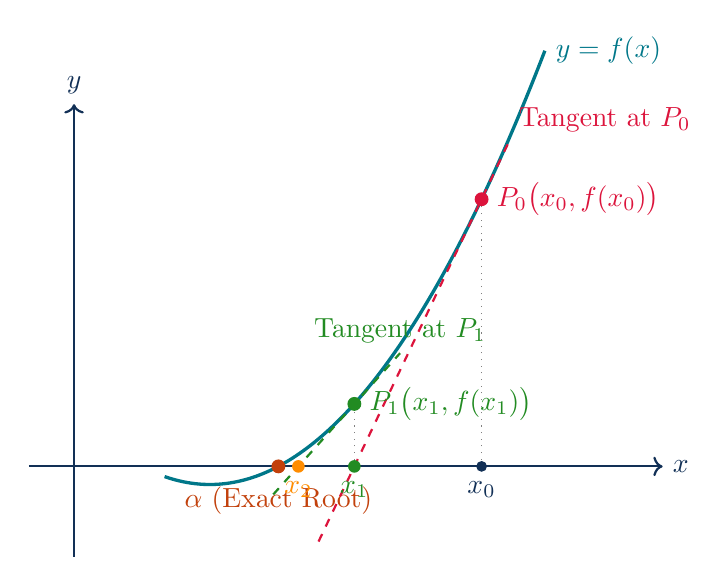
\begin{tikzpicture}[scale=1.15]
    % Axes
    \draw[->, thick, primary] (-0.5, 0) -- (6.5, 0) node[right, primary] {$x$};
    \draw[->, thick, primary] (0, -1.0) -- (0, 4.0) node[above, primary] {$y$};
    
    % Curve f(x) = (x-2)^2 - 0.5 (scaled)
    \draw[very thick, secondary, domain=1.0:5.2, samples=100] 
        plot (\x, {0.35*(\x-1.5)*(\x-1.5) - 0.2}) 
        node[right] {$y = f(x)$};
    
    % Exact root alpha: at y=0 => 0.35*(x-1.5)^2 = 0.2 => x = 1.5 + sqrt(0.2/0.35) = 2.256
    \coordinate (Alpha) at (2.256, 0);
    \filldraw[accent] (Alpha) circle (2pt) node[below=4pt, accent] {$\alpha$ (Exact Root)};
    
    % Initial point x0 = 4.5
    \coordinate (X0) at (4.5, 0);
    % f(4.5) = 0.35*(3.0)^2 - 0.2 = 3.15 - 0.2 = 2.95
    \coordinate (P0) at (4.5, 2.95);
    % f'(4.5) = 0.7*(3.0) = 2.1
    % Tangent at x0: y - 2.95 = 2.1*(x - 4.5) => at y=0, x1 = 4.5 - 2.95/2.1 = 3.095
    \coordinate (X1) at (3.095, 0);
    \coordinate (P1) at (3.095, 0.69);
    % f'(3.095) = 0.7*(1.595) = 1.1165
    % Tangent at x1: y - 0.69 = 1.1165*(x - 3.095) => at y=0, x2 = 3.095 - 0.69/1.1165 = 2.477
    \coordinate (X2) at (2.477, 0);
    
    % Tangent lines
    \draw[thick, Crimson, dashed] (2.7, -0.83) -- (4.8, 3.58) node[above right] {Tangent at $P_0$};
    \draw[thick, ForestGreen, dashed] (2.2, -0.31) -- (3.6, 1.25) node[above] {Tangent at $P_1$};
    
    % Drop lines
    \draw[dotted, gray] (X0) -- (P0);
    \draw[dotted, gray] (X1) -- (P1);
    
    % Points
    \filldraw[primary] (X0) circle (1.5pt) node[below=2pt] {$x_0$};
    \filldraw[Crimson] (P0) circle (2pt) node[right=2pt] {$P_0\big(x_0, f(x_0)\big)$};
    \filldraw[ForestGreen] (X1) circle (1.8pt) node[below=2pt, ForestGreen] {$x_1$};
    \filldraw[ForestGreen] (P1) circle (2pt) node[right=2pt] {$P_1\big(x_1, f(x_1)\big)$};
    \filldraw[DarkOrange] (X2) circle (1.8pt) node[below=2pt, DarkOrange] {$x_2$};
\end{tikzpicture}
\end{center}

% =========================================================================
% PAGE 5: NEWTON-RAPHSON SOLVED PROBLEM
% =========================================================================
\section{Page 5: Newton--Raphson Iterative Implementation and Solved Problem}
\label{sec:page5_nr_example}

\begin{examplebox}[Detailed Analytical Solution for $x^3 + x^2 - 1 = 0$]
Given:
\begin{equation}
    f(x) = x^3 + x^2 - 1 \implies f'(x) = 3x^2 + 2x
\end{equation}
Substituting into the Newton--Raphson formula:
\begin{align}
    x_{k+1} &= x_k - \frac{x_k^3 + x_k^2 - 1}{3x_k^2 + 2x_k} \nonumber \\
    &= \frac{x_k(3x_k^2 + 2x_k) - (x_k^3 + x_k^2 - 1)}{3x_k^2 + 2x_k} \nonumber \\
    &= \frac{3x_k^3 + 2x_k^2 - x_k^3 - x_k^2 + 1}{3x_k^2 + 2x_k} \nonumber \\
    \Aboxed{x_{k+1} &= \frac{2x_k^3 + x_k^2 + 1}{3x_k^2 + 2x_k}}
\end{align}
Choose initial approximation $x_0 = 1$:

\textbf{Iteration 1 ($k = 0$):}
\begin{equation}
    x_1 = \frac{2(1)^3 + (1)^2 + 1}{3(1)^2 + 2(1)} = \frac{2 + 1 + 1}{3 + 2} = \frac{4}{5} = \mathbf{0.8}
\end{equation}

\textbf{Iteration 2 ($k = 1$):}
\begin{align}
    x_2 &= \frac{2(0.8)^3 + (0.8)^2 + 1}{3(0.8)^2 + 2(0.8)} = \frac{2(0.512) + 0.64 + 1}{3(0.64) + 1.6} \nonumber \\
    &= \frac{1.024 + 0.64 + 1}{1.92 + 1.6} = \frac{2.664}{3.52} \approx \mathbf{0.756818}
\end{align}

\textbf{Iteration 3 ($k = 2$):}
\begin{align}
    x_3 &= \frac{2(0.756818)^3 + (0.756818)^2 + 1}{3(0.756818)^2 + 2(0.756818)} \nonumber \\
    &= \frac{2(0.433485) + 0.572774 + 1}{3(0.572774) + 1.513636} = \frac{2.439744}{3.231958} \approx \mathbf{0.754880}
\end{align}
After just 3 iterations, $x_3 = 0.754880$ matches the true root $\alpha = 0.754878$ to 5 decimal places! Compare this to the Regula-Falsi method which needed 5 iterations to reach $0.754263$.
\end{examplebox}

% =========================================================================
% PAGES 6-7: CONVERGENCE ORDER OF REGULA-FALSI
% =========================================================================
\section{Pages 6--7: Rigorous Derivation of the Order of Convergence for Regula--Falsi}
\label{sec:page6_7_regula_convergence}

\begin{theorembox}[Linear Convergence of the Regula--Falsi Method ($p = 1$)]
Let $\alpha$ be a simple root of $f(x) = 0$ in $[a, b]$. In the Regula--Falsi (false position) method, suppose without loss of generality that $f''(x) > 0$ (concave upward) throughout $[a, b]$, with $f(a) < 0$ and $f(b) > 0$. Under these conditions, the left endpoint $a$ remains stagnant ($x_0 = a$), while the sequence of iterates $\{x_k\}$ approaches $\alpha$ monotonically from the right.

The order of convergence is strictly \textbf{linear}:
\begin{equation}
    \boxed{p = 1} \quad \text{with asymptotic error constant } C = \left| \frac{(a - \alpha)^2 f''(\alpha)}{2 f(a)} \right|
\end{equation}
\end{theorembox}

\begin{proof}[Exhaustive Step-by-Step Proof of Linear Convergence ($p = 1$)]
\noindent\textbf{Step 1: Cartesian Equation of the Chord and the Iteration Formula} \\
The secant line connecting the stagnant point $(a, f(a))$ and the current iterate $(x_k, f(x_k))$ has slope:
\begin{equation}
    m_k = \frac{f(x_k) - f(a)}{x_k - a}
\end{equation}
The point-slope equation of this chord is:
\begin{equation}
    y - f(a) = \frac{f(x_k) - f(a)}{x_k - a}(x - a)
\end{equation}
Setting $y = 0$ to find the next approximation $x_{k+1}$ (the $x$-intercept):
\begin{equation}
    0 - f(a) = \frac{f(x_k) - f(a)}{x_k - a}(x_{k+1} - a) \implies x_{k+1} - a = -f(a) \frac{x_k - a}{f(x_k) - f(a)}
\end{equation}
Adding $a$ to both sides and putting over a common denominator:
\begin{equation}
    x_{k+1} = a - \frac{f(a)(x_k - a)}{f(x_k) - f(a)} = \frac{a[f(x_k) - f(a)] - f(a)(x_k - a)}{f(x_k) - f(a)} = \frac{a f(x_k) - x_k f(a)}{f(x_k) - f(a)}
\end{equation}

\noindent\textbf{Step 2: Exact Algebraic Error Recurrence} \\
Define the error at iteration $k$ as $e_k = x_k - \alpha$, and the fixed displacement of the stagnant endpoint as $e_a = a - \alpha$. Subtracting the true root $\alpha$ from both sides:
\begin{align}
    e_{k+1} &= x_{k+1} - \alpha = \frac{a f(x_k) - x_k f(a)}{f(x_k) - f(a)} - \alpha \nonumber \\
    &= \frac{a f(x_k) - x_k f(a) - \alpha[f(x_k) - f(a)]}{f(x_k) - f(a)} \nonumber \\
    &= \frac{(a - \alpha) f(x_k) - (x_k - \alpha) f(a)}{f(x_k) - f(a)} \nonumber \\
    &= \frac{e_a f(x_k) - e_k f(a)}{f(x_k) - f(a)}
    \label{eq:regula_exact_error_ratio}
\end{align}

\noindent\textbf{Step 3: Taylor Series Expansion of $f(x_k)$ about the Root $\alpha$} \\
Since $\alpha$ is a root ($f(\alpha) = 0$), expanding $f(x_k) = f(\alpha + e_k)$ in powers of $e_k$:
\begin{equation}
    f(x_k) = f(\alpha) + e_k f'(\alpha) + \frac{e_k^2}{2!} f''(\alpha) + \frac{e_k^3}{3!} f'''(\alpha) + \mathcal{O}(e_k^4) = e_k f'(\alpha) + \frac{e_k^2}{2} f''(\alpha) + \mathcal{O}(e_k^3)
\end{equation}

\noindent\textbf{Step 4: Expansion of the Numerator} \\
Substitute the expansion of $f(x_k)$ into the numerator of Equation~\eqref{eq:regula_exact_error_ratio}:
\begin{align}
    \text{Numerator} &= e_a \left[ e_k f'(\alpha) + \frac{e_k^2}{2} f''(\alpha) + \mathcal{O}(e_k^3) \right] - e_k f(a) \nonumber \\
    &= e_k \left[ e_a f'(\alpha) - f(a) \right] + \frac{e_a f''(\alpha)}{2} e_k^2 + \mathcal{O}(e_k^3)
\end{align}
Now expand $f(a) = f(\alpha + e_a)$ about $\alpha$ in powers of $e_a$:
\begin{equation}
    f(a) = f(\alpha) + e_a f'(\alpha) + \frac{e_a^2}{2} f''(\alpha) + \mathcal{O}(e_a^3) = e_a f'(\alpha) + \frac{e_a^2}{2} f''(\alpha) + \mathcal{O}(e_a^3)
\end{equation}
Subtracting $f(a)$ from $e_a f'(\alpha)$:
\begin{equation}
    e_a f'(\alpha) - f(a) = e_a f'(\alpha) - \left[ e_a f'(\alpha) + \frac{e_a^2}{2} f''(\alpha) + \mathcal{O}(e_a^3) \right] = -\frac{e_a^2}{2} f''(\alpha) + \mathcal{O}(e_a^3)
\end{equation}
Substituting this back into the numerator:
\begin{align}
    \text{Numerator} &= e_k \left[ -\frac{e_a^2}{2} f''(\alpha) + \mathcal{O}(e_a^3) \right] + \frac{e_a f''(\alpha)}{2} e_k^2 + \mathcal{O}(e_k^3) \nonumber \\
    &= -\frac{e_a^2 f''(\alpha)}{2} e_k + \mathcal{O}(e_k^2)
\end{align}

\noindent\textbf{Step 5: Expansion and Inversion of the Denominator} \\
The denominator is:
\begin{equation}
    \text{Denominator} = f(x_k) - f(a) = \left[ e_k f'(\alpha) + \mathcal{O}(e_k^2) \right] - f(a) = -f(a) \left[ 1 - \frac{f'(\alpha)}{f(a)} e_k + \mathcal{O}(e_k^2) \right]
\end{equation}
Using the geometric/binomial series $(1 - u)^{-1} = 1 + u + \mathcal{O}(u^2)$:
\begin{equation}
    \frac{1}{f(x_k) - f(a)} = -\frac{1}{f(a)} \left[ 1 + \frac{f'(\alpha)}{f(a)} e_k + \mathcal{O}(e_k^2) \right]
\end{equation}

\noindent\textbf{Step 6: Asymptotic Error Ratio and Order of Convergence} \\
Multiplying the numerator and inverted denominator:
\begin{align}
    e_{k+1} &= \left( -\frac{e_a^2 f''(\alpha)}{2} e_k + \mathcal{O}(e_k^2) \right) \left( -\frac{1}{f(a)} \right) \left( 1 + \frac{f'(\alpha)}{f(a)} e_k + \mathcal{O}(e_k^2) \right) \nonumber \\
    &= \left[ \frac{e_a^2 f''(\alpha)}{2 f(a)} \right] e_k + \mathcal{O}(e_k^2)
\end{align}
Taking absolute values and the limit as $k \to \infty$:
\begin{equation}
    \lim_{k \to \infty} \frac{|e_{k+1}|}{|e_k|^1} = \left| \frac{e_a^2 f''(\alpha)}{2 f(a)} \right| = \left| \frac{(a - \alpha)^2 f''(\alpha)}{2 f(a)} \right| = C
\end{equation}
Because the denominator exponent of $|e_k|$ is $1$ and the asymptotic constant $C \in (0, 1)$ is non-zero, the order of convergence of the Regula--Falsi method is strictly:
\begin{equation}
    \boxed{p = 1} \quad \text{\textbf{(Linear Convergence)}}
\end{equation}
\end{proof}

\begin{notebox}[Physical Insight: Why Regula--Falsi Stalls while Secant Accelerates]
In the Secant method, both endpoints $x_{k-1}$ and $x_k$ update dynamically at every single step, allowing the chord length $x_k - x_{k-1} \to 0$ to shrink alongside the error, driving superlinear convergence ($p \approx 1.618$).

In contrast, the Regula--Falsi method strictly enforces the bracketing condition $f(a) f(x_k) < 0$. If $f''(x) > 0$, the chord always lies above the curve, ensuring that every new approximation $x_{k+1}$ falls strictly on the \textbf{same side} of the root. As a direct consequence, the endpoint $a$ never updates—it becomes \textbf{stagnant}. The chord pivots perpetually around the fixed anchor point $(a, f(a))$, dropping the rate of convergence from superlinear ($p = 1.618$) to purely linear ($p = 1$).
\end{notebox}

% =========================================================================
% PAGES 8-9: CONVERGENCE ORDER OF SECANT METHOD
% =========================================================================
\section{Pages 8--9: Rigorous Derivation of the Order of Convergence for the Secant Method}
\label{sec:page8_9_secant_convergence}

\begin{theorembox}[Superlinear Convergence of the Secant Method \texorpdfstring{($p \approx 1.618$)}{(p approx 1.618)}]
Let $\alpha$ be a simple root of $f(x) = 0$ ($f(\alpha) = 0, f'(\alpha) \ne 0$). The order of convergence of the Secant method is superlinear:
\begin{equation}
    \boxed{p = \frac{1 + \sqrt{5}}{2} \approx 1.618034} \quad \text{\textbf{(The Golden Ratio $\Phi$)}}
\end{equation}
with asymptotic error constant $C = \left(\frac{f''(\alpha)}{2f'(\alpha)}\right)^{p-1}$.
\end{theorembox}

\begin{proof}[Rigorous Mathematical Derivation (Manuscript Pages 8--9)]
\noindent\textbf{Step 1: Error Difference Equation} \\
The Secant recurrence is:
\begin{equation}
    x_{k+1} = x_k - \frac{x_k - x_{k-1}}{f(x_k) - f(x_{k-1})} f(x_k)
\end{equation}
Let $e_k = x_k - \alpha, e_{k-1} = x_{k-1} - \alpha, e_{k+1} = x_{k+1} - \alpha$. Subtracting $\alpha$:
\begin{align}
    e_{k+1} &= x_k - \alpha - \frac{x_k - x_{k-1}}{f(x_k) - f(x_{k-1})} f(x_k) \nonumber \\
    &= e_k - \frac{e_k - e_{k-1}}{f(x_k) - f(x_{k-1})} f(x_k) \nonumber \\
    &= \frac{e_k[f(x_k) - f(x_{k-1})] - (e_k - e_{k-1}) f(x_k)}{f(x_k) - f(x_{k-1})} \nonumber \\
    &= \frac{e_k f(x_k) - e_k f(x_{k-1}) - e_k f(x_k) + e_{k-1} f(x_k)}{f(x_k) - f(x_{k-1})} \nonumber \\
    &= \frac{e_{k-1} f(x_k) - e_k f(x_{k-1})}{f(x_k) - f(x_{k-1})}
    \label{eq:secant_error_ratio_master}
\end{align}

\noindent\textbf{Step 2: Taylor Series Expansions to Third Order} \\
Since $f(\alpha) = 0$, expanding $f(x_k)$ and $f(x_{k-1})$ in powers of errors:
\begin{align}
    f(x_k) &= f'(\alpha) e_k + \frac{f''(\alpha)}{2} e_k^2 + \frac{f'''(\alpha)}{6} e_k^3 + \mathcal{O}(e_k^4) \\
    f(x_{k-1}) &= f'(\alpha) e_{k-1} + \frac{f''(\alpha)}{2} e_{k-1}^2 + \frac{f'''(\alpha)}{6} e_{k-1}^3 + \mathcal{O}(e_{k-1}^4)
\end{align}

\noindent\textbf{Step 3: Expansion and Factorization of the Numerator} \\
Multiply by $e_{k-1}$ and $e_k$ respectively:
\begin{align}
    e_{k-1} f(x_k) &= f'(\alpha) e_k e_{k-1} + \frac{f''(\alpha)}{2} e_k^2 e_{k-1} + \frac{f'''(\alpha)}{6} e_k^3 e_{k-1} + \dots \\
    e_k f(x_{k-1}) &= f'(\alpha) e_k e_{k-1} + \frac{f''(\alpha)}{2} e_k e_{k-1}^2 + \frac{f'''(\alpha)}{6} e_k e_{k-1}^3 + \dots
\end{align}
Subtracting the two equations, the first-order terms $f'(\alpha) e_k e_{k-1}$ cancel identically:
\begin{align}
    e_{k-1} f(x_k) - e_k f(x_{k-1}) &= \frac{f''(\alpha)}{2} e_k e_{k-1}(e_k - e_{k-1}) + \frac{f'''(\alpha)}{6} e_k e_{k-1}(e_k^2 - e_{k-1}^2) + \dots \nonumber \\
    &= e_k e_{k-1}(e_k - e_{k-1}) \left[ \frac{f''(\alpha)}{2} + \frac{f'''(\alpha)}{6}(e_k + e_{k-1}) + \dots \right]
\end{align}

\noindent\textbf{Step 4: Expansion and Factorization of the Denominator}
\begin{align}
    f(x_k) - f(x_{k-1}) &= f'(\alpha)(e_k - e_{k-1}) + \frac{f''(\alpha)}{2}(e_k^2 - e_{k-1}^2) + \dots \nonumber \\
    &= (e_k - e_{k-1}) \left[ f'(\alpha) + \frac{f''(\alpha)}{2}(e_k + e_{k-1}) + \dots \right]
\end{align}

\noindent\textbf{Step 5: Exact Cancellation of the Discrepancy Factor $(e_k - e_{k-1})$} \\
Substituting numerator and denominator into Equation~\eqref{eq:secant_error_ratio_master}:
\begin{align}
    e_{k+1} &= \frac{e_k e_{k-1}(e_k - e_{k-1}) \left[ \frac{f''(\alpha)}{2} + \dots \right]}{(e_k - e_{k-1}) \left[ f'(\alpha) + \frac{f''(\alpha)}{2}(e_k + e_{k-1}) + \dots \right]} \nonumber \\
    &= e_k e_{k-1} \frac{\frac{f''(\alpha)}{2} + \mathcal{O}(e_k + e_{k-1})}{f'(\alpha) \left[ 1 + \frac{f''(\alpha)}{2 f'(\alpha)}(e_k + e_{k-1}) + \dots \right]} \nonumber \\
    &= \left[ \frac{f''(\alpha)}{2 f'(\alpha)} \right] e_k e_{k-1} + \mathcal{O}\big(e_k e_{k-1}(e_k + e_{k-1})\big)
\end{align}
Neglecting higher-order terms, we obtain the pivotal coupled error recurrence:
\begin{equation}
    \label{eq:secant_asymptotic_recurrence_explicit}
    \boxed{e_{k+1} \approx M e_k e_{k-1}} \quad \text{where } M = \frac{f''(\alpha)}{2 f'(\alpha)}
\end{equation}

\noindent\textbf{Step 6: Determination of the Order of Convergence $p$} \\
We present two complementary, rigorous proofs of the convergence order:

\paragraph{Method 1: Direct Power Ansatz}
Assume an asymptotic convergence relation of the form:
\begin{equation}
    e_{k+1} = A e_k^p \iff e_k = A e_{k-1}^p \iff e_{k-1} = \left(\frac{e_k}{A}\right)^{1/p} = A^{-1/p} e_k^{1/p}
\end{equation}
Substitute $e_{k+1} = A e_k^p$ and $e_{k-1} = A^{-1/p} e_k^{1/p}$ into Equation~\eqref{eq:secant_asymptotic_recurrence_explicit}:
\begin{equation}
    A e_k^p = M e_k \left( A^{-1/p} e_k^{1/p} \right) = M A^{-1/p} e_k^{1 + 1/p}
\end{equation}
Equating exponents of $e_k$ on both sides:
\begin{equation}
    p = 1 + \frac{1}{p} \iff p^2 - p - 1 = 0
\end{equation}
The roots of this characteristic equation are:
\begin{equation}
    p = \frac{1 \pm \sqrt{(-1)^2 - 4(1)(-1)}}{2} = \frac{1 \pm \sqrt{5}}{2}
\end{equation}
Since an iterative sequence cannot have a negative convergence exponent ($p > 0$ for decreasing error sequences), we discard the negative root:
\begin{equation}
    \boxed{p = \frac{1 + \sqrt{5}}{2} \approx 1.6180339887\dots} \quad \text{\textbf{(The Golden Ratio $\Phi$)}}
\end{equation}
Equating coefficients:
\begin{equation}
    A = M A^{-1/p} \implies A^{1 + 1/p} = M \implies A^p = M \implies A = M^{1/p} = M^{p-1} = \left( \frac{f''(\alpha)}{2 f'(\alpha)} \right)^{p-1}
\end{equation}

\paragraph{Method 2: Logarithmic Transformation and Fibonacci Sequence}
Multiply both sides of $e_{k+1} = M e_k e_{k-1}$ by $M$:
\begin{equation}
    M e_{k+1} = (M e_k)(M e_{k-1})
\end{equation}
Taking the natural logarithm of absolute values, let $\epsilon_k = \ln|M e_k|$:
\begin{equation}
    \ln|M e_{k+1}| = \ln|M e_k| + \ln|M e_{k-1}| \iff \boxed{\epsilon_{k+1} = \epsilon_k + \epsilon_{k-1}}
\end{equation}
This is precisely the \textbf{Fibonacci recurrence relation}!
The general solution of this linear difference equation is:
\begin{equation}
    \epsilon_k = C_1 r_1^k + C_2 r_2^k, \quad \text{where } r_{1,2} = \frac{1 \pm \sqrt{5}}{2}
\end{equation}
Since $|r_2| = \left|\frac{1-\sqrt{5}}{2}\right| \approx 0.618 < 1$, the term $r_2^k \to 0$ rapidly as $k \to \infty$. Thus:
\begin{equation}
    \epsilon_k \approx C_1 r_1^k \implies \epsilon_{k+1} \approx C_1 r_1^{k+1} = r_1 (C_1 r_1^k) \approx r_1 \epsilon_k
\end{equation}
Substituting back $\epsilon_k = \ln|M e_k|$:
\begin{equation}
    \ln|M e_{k+1}| \approx r_1 \ln|M e_k| = \ln\left(|M e_k|^{r_1}\right)
\end{equation}
Exponentiating both sides:
\begin{equation}
    |M e_{k+1}| \approx |M e_k|^{r_1} \implies |e_{k+1}| \approx M^{r_1 - 1} |e_k|^{r_1}
\end{equation}
This rigorously establishes that the order of convergence is identically the Golden Ratio $r_1 = \frac{1+\sqrt{5}}{2} \approx 1.618$.
\end{proof}

% =========================================================================
% PAGES 10-12: CONVERGENCE ORDER OF NEWTON-RAPHSON & CUBE ROOT
% =========================================================================
\section{Pages 10--12: Quadratic Convergence of Newton--Raphson and Fast Radical Extraction}
\label{sec:page10_12_nr_convergence}

\begin{theorembox}[Quadratic Convergence of the Newton--Raphson Method ($p = 2$)]
Let $\alpha$ be a simple root of $f(x) = 0$ ($f(\alpha) = 0, f'(\alpha) \ne 0$) with $f \in C^2[a, b]$. If the initial approximation $x_0$ is chosen sufficiently close to $\alpha$, the Newton--Raphson iteration:
\begin{equation}
    x_{k+1} = x_k - \frac{f(x_k)}{f'(x_k)}
\end{equation}
converges to $\alpha$ with \textbf{quadratic order of convergence} ($p = 2$):
\begin{equation}
    \boxed{\lim_{k \to \infty} \frac{|e_{k+1}|}{|e_k|^2} = \left| \frac{f''(\alpha)}{2 f'(\alpha)} \right| \equiv C}
\end{equation}
where $e_k = x_k - \alpha$ is the signed error at iteration $k$, and $C$ is the asymptotic error constant.
\end{theorembox}

\begin{proof}[Exhaustive Step-by-Step Proof of Quadratic Convergence for Newton--Raphson]
We present two complementary proofs: first, the asymptotic Taylor series expansion with explicit binomial inversion showing all cross-terms; second, the exact non-asymptotic closed form using Taylor's Theorem with Lagrange remainder.

\medskip
\noindent\textbf{Method 1: Asymptotic Taylor Series Expansion with Explicit Binomial Inversion}

\noindent\textbf{Step 1: Express iteration in terms of error variables.} \\
Let $x_k = \alpha + e_k$ and $x_{k+1} = \alpha + e_{k+1}$. Subtracting the true root $\alpha$ from both sides of the Newton--Raphson formula gives:
\begin{equation}
    x_{k+1} - \alpha = (x_k - \alpha) - \frac{f(x_k)}{f'(x_k)} \implies e_{k+1} = e_k - \frac{f(\alpha + e_k)}{f'(\alpha + e_k)}
\end{equation}

\noindent\textbf{Step 2: Taylor series expansion of numerator $f(\alpha + e_k)$.} \\
Expanding $f(\alpha + e_k)$ about the root $\alpha$, using $f(\alpha) = 0$:
\begin{align}
    f(\alpha + e_k) &= f(\alpha) + e_k f'(\alpha) + \frac{e_k^2}{2!} f''(\alpha) + \frac{e_k^3}{3!} f'''(\alpha) + \mathcal{O}(e_k^4) \nonumber \\
    &= e_k f'(\alpha) \left[ 1 + \frac{f''(\alpha)}{2 f'(\alpha)} e_k + \frac{f'''(\alpha)}{6 f'(\alpha)} e_k^2 + \mathcal{O}(e_k^3) \right]
\end{align}
For compact notation, define the normalized derivative ratios:
\begin{equation}
    c_2 = \frac{f''(\alpha)}{2 f'(\alpha)}, \qquad c_3 = \frac{f'''(\alpha)}{6 f'(\alpha)}
\end{equation}
Then the numerator simplifies to:
\begin{equation}
    f(\alpha + e_k) = f'(\alpha) e_k \left[ 1 + c_2 e_k + c_3 e_k^2 + \mathcal{O}(e_k^3) \right]
\end{equation}

\noindent\textbf{Step 3: Taylor series expansion of denominator $f'(\alpha + e_k)$.} \\
Differentiating the Taylor series or expanding $f'(\alpha + e_k)$ directly about $\alpha$:
\begin{align}
    f'(\alpha + e_k) &= f'(\alpha) + e_k f''(\alpha) + \frac{e_k^2}{2!} f'''(\alpha) + \mathcal{O}(e_k^3) \nonumber \\
    &= f'(\alpha) \left[ 1 + \frac{f''(\alpha)}{f'(\alpha)} e_k + \frac{f'''(\alpha)}{2 f'(\alpha)} e_k^2 + \mathcal{O}(e_k^3) \right] \nonumber \\
    &= f'(\alpha) \left[ 1 + 2 c_2 e_k + 3 c_3 e_k^2 + \mathcal{O}(e_k^3) \right]
\end{align}

\noindent\textbf{Step 4: Division via series expansion $(1 + z)^{-1}$.} \\
Set $z = 2 c_2 e_k + 3 c_3 e_k^2 + \mathcal{O}(e_k^3)$. As $e_k \to 0$, $|z| < 1$, so we expand:
\begin{equation}
    (1 + z)^{-1} = 1 - z + z^2 - z^3 + \dots
\end{equation}
Computing powers of $z$ up to second order in $e_k$:
\begin{align}
    z &= 2 c_2 e_k + 3 c_3 e_k^2 + \mathcal{O}(e_k^3) \\
    z^2 &= \left( 2 c_2 e_k + 3 c_3 e_k^2 \right)^2 = 4 c_2^2 e_k^2 + \mathcal{O}(e_k^3)
\end{align}
Substituting into the inverse series:
\begin{align}
    \left[ 1 + 2 c_2 e_k + 3 c_3 e_k^2 + \mathcal{O}(e_k^3) \right]^{-1} &= 1 - \left( 2 c_2 e_k + 3 c_3 e_k^2 \right) + 4 c_2^2 e_k^2 + \mathcal{O}(e_k^3) \nonumber \\
    &= 1 - 2 c_2 e_k + (4 c_2^2 - 3 c_3) e_k^2 + \mathcal{O}(e_k^3)
\end{align}

\noindent\textbf{Step 5: Multiply numerator by inverted denominator.} \\
The quotient evaluates to:
\begin{align}
    \frac{f(\alpha + e_k)}{f'(\alpha + e_k)} &= \frac{f'(\alpha) e_k \left[ 1 + c_2 e_k + c_3 e_k^2 + \mathcal{O}(e_k^3) \right]}{f'(\alpha) \left[ 1 + 2 c_2 e_k + 3 c_3 e_k^2 + \mathcal{O}(e_k^3) \right]} \nonumber \\
    &= e_k \left[ 1 + c_2 e_k + c_3 e_k^2 + \mathcal{O}(e_k^3) \right] \left[ 1 - 2 c_2 e_k + (4 c_2^2 - 3 c_3) e_k^2 + \mathcal{O}(e_k^3) \right]
\end{align}
Expanding the polynomial product term by term:
\begin{align}
    \left[ 1 + c_2 e_k + c_3 e_k^2 \right] &\left[ 1 - 2 c_2 e_k + (4 c_2^2 - 3 c_3) e_k^2 \right] \nonumber \\
    &= 1 \cdot \left[ 1 - 2 c_2 e_k + (4 c_2^2 - 3 c_3) e_k^2 \right] \nonumber \\
    &\quad + c_2 e_k \cdot \left[ 1 - 2 c_2 e_k \right] + c_3 e_k^2 \cdot [1] + \mathcal{O}(e_k^3) \nonumber \\
    &= 1 - 2 c_2 e_k + 4 c_2^2 e_k^2 - 3 c_3 e_k^2 + c_2 e_k - 2 c_2^2 e_k^2 + c_3 e_k^2 + \mathcal{O}(e_k^3) \nonumber \\
    &= 1 + (-2 c_2 + c_2) e_k + (4 c_2^2 - 2 c_2^2 - 3 c_3 + c_3) e_k^2 + \mathcal{O}(e_k^3) \nonumber \\
    &= 1 - c_2 e_k + (2 c_2^2 - 2 c_3) e_k^2 + \mathcal{O}(e_k^3)
\end{align}
Multiplying by the leading $e_k$:
\begin{equation}
    \frac{f(\alpha + e_k)}{f'(\alpha + e_k)} = e_k - c_2 e_k^2 + 2(c_2^2 - c_3) e_k^3 + \mathcal{O}(e_k^4)
\end{equation}

\noindent\textbf{Step 6: Substitute back into error recurrence.} \\
\begin{align}
    e_{k+1} &= e_k - \frac{f(\alpha + e_k)}{f'(\alpha + e_k)} \nonumber \\
    &= e_k - \left[ e_k - c_2 e_k^2 + 2(c_2^2 - c_3) e_k^3 + \mathcal{O}(e_k^4) \right] \nonumber \\
    &= c_2 e_k^2 - 2(c_2^2 - c_3) e_k^3 + \mathcal{O}(e_k^4)
\end{align}
Substituting $c_2 = \frac{f''(\alpha)}{2 f'(\alpha)}$:
\begin{equation}
    \boxed{e_{k+1} = \left[ \frac{f''(\alpha)}{2 f'(\alpha)} \right] e_k^2 + \mathcal{O}(e_k^3)}
\end{equation}
Taking the absolute ratio in the limit as $k \to \infty$ ($e_k \to 0$):
\begin{equation}
    \lim_{k \to \infty} \frac{|e_{k+1}|}{|e_k|^2} = \left| \frac{f''(\alpha)}{2 f'(\alpha)} \right| \ne 0
\end{equation}
This proves unequivocally that the order of convergence is \textbf{strictly quadratic} ($p = 2$).

\bigskip
\noindent\textbf{Method 2: Exact Closed-Form Error Formula via Taylor's Theorem with Lagrange Remainder}

\noindent Taylor's theorem with exact second-order Lagrange remainder for $f(\alpha)$ expanded about $x_k$ states that there exists $\xi_k$ strictly between $x_k$ and $\alpha$ such that:
\begin{equation}
    f(\alpha) = f(x_k) + (\alpha - x_k) f'(x_k) + \frac{(\alpha - x_k)^2}{2!} f''(\xi_k)
\end{equation}
Since $\alpha$ is a root, $f(\alpha) = 0$. Recalling $\alpha - x_k = -e_k$:
\begin{equation}
    0 = f(x_k) - e_k f'(x_k) + \frac{e_k^2}{2} f''(\xi_k)
\end{equation}
Isolating $f(x_k)$:
\begin{equation}
    f(x_k) = e_k f'(x_k) - \frac{e_k^2}{2} f''(\xi_k)
\end{equation}
Dividing throughout by $f'(x_k)$ (which is non-zero in a neighborhood of $\alpha$):
\begin{equation}
    \frac{f(x_k)}{f'(x_k)} = e_k - \frac{f''(\xi_k)}{2 f'(x_k)} e_k^2
\end{equation}
Substituting this directly into the Newton--Raphson iteration formula:
\begin{align}
    x_{k+1} &= x_k - \frac{f(x_k)}{f'(x_k)} \nonumber \\
    x_{k+1} - \alpha &= (x_k - \alpha) - \left( e_k - \frac{f''(\xi_k)}{2 f'(x_k)} e_k^2 \right) \nonumber \\
    e_{k+1} &= e_k - e_k + \frac{f''(\xi_k)}{2 f'(x_k)} e_k^2
\end{align}
\begin{equation}
    \boxed{e_{k+1} = \frac{f''(\xi_k)}{2 f'(x_k)} e_k^2}
\end{equation}
This is the \textbf{exact error equation} holding at every finite iteration $k$ without truncating any higher-order terms! Since $x_k \to \alpha$ and $\xi_k$ lies between $x_k$ and $\alpha$, $\lim_{k \to \infty} \xi_k = \alpha$, which immediately gives:
\begin{equation}
    \lim_{k \to \infty} \frac{|e_{k+1}|}{|e_k|^2} = \lim_{k \to \infty} \frac{|f''(\xi_k)|}{2|f'(x_k)|} = \frac{|f''(\alpha)|}{2|f'(\alpha)|} = C
\end{equation}
\end{proof}


\begin{examplebox}[{Manuscript Problem: Computation of Cube Root $\sqrt[3]{N}$ (Page 11)}]
Let $x = \sqrt[3]{N} \implies x^3 - N = 0$.
Here $f(x) = x^3 - N$ and $f'(x) = 3x^2$. Applying Newton--Raphson:
\begin{equation}
    x_{k+1} = x_k - \frac{x_k^3 - N}{3x_k^2} = \frac{3x_k^3 - x_k^3 + N}{3x_k^2} = \boxed{\frac{2x_k^3 + N}{3x_k^2} = \frac{1}{3}\left( 2x_k + \frac{N}{x_k^2} \right)}
\end{equation}
\textbf{Numerical Application (Compute $\sqrt[3]{37}$):}
Here $N = 37$. Since $3^3 = 27 < 37 < 64 = 4^3$, choose $x_0 = 3$.

\textbf{Iteration 1 ($k = 0$):}
\begin{equation}
    x_1 = \frac{2(3)^3 + 37}{3(3)^2} = \frac{2(27) + 37}{3(9)} = \frac{54 + 37}{27} = \frac{91}{27} \approx \mathbf{3.370370}
\end{equation}

\textbf{Iteration 2 ($k = 1$):}
\begin{equation}
    x_2 = \frac{1}{3}\left( 2(3.370370) + \frac{37}{(3.370370)^2} \right) = \frac{1}{3}(6.740741 + 3.257223) = \frac{9.997964}{3} \approx \mathbf{3.332655}
\end{equation}
Since $(3.332655)^3 \approx 37.016$, after two iterations the result is within $0.015\%$ of the true value $\sqrt[3]{37} \approx 3.332222$.
\end{examplebox}

% =========================================================================
% PAGES 12-13: CONVERGENCE CONDITIONS & RECIPROCAL ALGORITHM
% =========================================================================
\section{Pages 12--13: Domain of Convergence and Division-Free Reciprocal Algorithm}
\label{sec:page12_13_convergence_conditions}

\begin{theorembox}[Fourier's Sufficient Condition for Newton--Raphson Convergence]
The Newton--Raphson iteration converges unconditionally to the unique root $\alpha$ in $[a, b]$ if:
\begin{enumerate}
    \item $f(a) \cdot f(b) < 0$ (Root existence).
    \item $f'(x) \ne 0$ for all $x \in [a, b]$ (Monotonicity and non-vanishing slope).
    \item $f''(x)$ does not change sign on $[a, b]$ (Strict convexity or concavity).
    \item The initial guess $x_0$ is chosen such that:
    \begin{equation}
        \boxed{f(x_0) \cdot f''(x_0) > 0}
    \end{equation}
\end{enumerate}
\end{theorembox}

\begin{proof}[Exhaustive Mathematical Proof of Fourier's Convergence Theorem]
We prove that under Fourier's conditions, the sequence generated by Newton--Raphson is strictly monotonic and bounded by the root $\alpha$, guaranteeing unconditional convergence via the Monotone Convergence Theorem of real analysis.

\medskip
\noindent\textbf{Step 1: Existence and Uniqueness of the Root.} \\
Since $f \in C^2[a, b]$ and $f(a) \cdot f(b) < 0$, the Intermediate Value Theorem guarantees the existence of at least one root $\alpha \in (a, b)$ such that $f(\alpha) = 0$.
Furthermore, because $f'(x) \ne 0$ on $[a, b]$, $f'(x)$ cannot change sign (by Darboux's Theorem on derivatives). Hence $f(x)$ is strictly monotonic on $[a, b]$, which guarantees that the root $\alpha$ is \textbf{strictly unique}.

\medskip
\noindent\textbf{Step 2: Convexity Analysis ($f''(x) > 0$).} \\
Without loss of generality, assume $f''(x) > 0$ for all $x \in [a, b]$ (the curve is strictly convex; if $f''(x) < 0$, consider the function $-f(x)$ which has identical roots and identical Newton iterations).
By Condition 4, $x_0$ is chosen such that $f(x_0) \cdot f''(x_0) > 0$. Since $f'' > 0$, this implies:
\begin{equation}
    f(x_0) > 0
\end{equation}
Now consider the sign of $f'(x)$:
\begin{itemize}
    \item \textbf{Subcase A ($f'(x) > 0$ on $[a, b]$):}
    Here $f$ is strictly increasing. Since $f(a) < 0 < f(b)$, the root $\alpha$ satisfies $f(x) < 0$ for $x \in [a, \alpha)$ and $f(x) > 0$ for $x \in (\alpha, b]$.
    Thus $f(x_0) > 0$ implies $x_0 \in (\alpha, b]$, i.e., $x_0 > \alpha$.
    
    \item \textbf{Subcase B ($f'(x) < 0$ on $[a, b]$):}
    Here $f$ is strictly decreasing with $f(a) > 0 > f(b)$. The condition $f(x_0) > 0$ implies $x_0 \in [a, \alpha)$, i.e., $x_0 < \alpha$.
\end{itemize}

\medskip
\noindent\textbf{Step 3: Establish Boundedness and Monotonicity by Induction.} \\
We analyze Subcase A ($f' > 0, f'' > 0, x_0 > \alpha$). We prove by induction that for all $k \ge 0$:
\begin{equation}
    \alpha < x_{k+1} < x_k \le b
\end{equation}
\begin{enumerate}
    \item \textbf{Inductive Hypothesis:} Assume $x_k > \alpha$.
    \item \textbf{Error Relation via Taylor's Theorem:}
    Expand $f(\alpha)$ in a Taylor series about the current iterate $x_k$ with exact Lagrange remainder:
    \begin{equation}
        0 = f(\alpha) = f(x_k) + f'(x_k)(\alpha - x_k) + \frac{1}{2} f''(\xi_k)(\alpha - x_k)^2
    \end{equation}
    for some point $\xi_k \in (\alpha, x_k) \subset (a, b)$.
    
    From the definition of the Newton--Raphson step, $x_{k+1} = x_k - \frac{f(x_k)}{f'(x_k)}$, which gives the exact identity:
    \begin{equation}
        f(x_k) = f'(x_k)(x_k - x_{k+1})
    \end{equation}
    Substituting this into the Taylor expansion:
    \begin{align}
        0 &= f'(x_k)(x_k - x_{k+1}) + f'(x_k)(\alpha - x_k) + \frac{1}{2} f''(\xi_k)(\alpha - x_k)^2 \nonumber \\
        &= f'(x_k)\big[ (x_k - x_{k+1}) + (\alpha - x_k) \big] + \frac{1}{2} f''(\xi_k)(\alpha - x_k)^2 \nonumber \\
        &= f'(x_k)(\alpha - x_{k+1}) + \frac{1}{2} f''(\xi_k)(\alpha - x_k)^2
    \end{align}
    Rearranging terms:
    \begin{equation}
        f'(x_k)(x_{k+1} - \alpha) = \frac{1}{2} f''(\xi_k)(x_k - \alpha)^2
    \end{equation}
    Dividing by $f'(x_k) > 0$:
    \begin{equation}
        \boxed{x_{k+1} - \alpha = \frac{f''(\xi_k)}{2 f'(x_k)} (x_k - \alpha)^2}
    \end{equation}
    Since $f''(\xi_k) > 0$, $f'(x_k) > 0$, and $(x_k - \alpha)^2 > 0$ (since $x_k \ne \alpha$), the right-hand side is \textbf{strictly positive}:
    \begin{equation}
        x_{k+1} - \alpha > 0 \implies \boxed{x_{k+1} > \alpha}
    \end{equation}
    Thus, every iterate remains strictly to the right of the root $\alpha$.
    
    \item \textbf{Strict Monotonic Decrease:}
    Compute the difference between successive iterates:
    \begin{equation}
        x_k - x_{k+1} = \frac{f(x_k)}{f'(x_k)}
    \end{equation}
    Since $x_k > \alpha$ and $f(x)$ is strictly increasing, $f(x_k) > f(\alpha) = 0$. Since $f'(x_k) > 0$:
    \begin{equation}
        x_k - x_{k+1} = \frac{f(x_k)}{f'(x_k)} > 0 \implies \boxed{x_{k+1} < x_k}
    \end{equation}
\end{enumerate}
Therefore, by mathematical induction, the sequence $\{x_k\}$ satisfies:
\begin{equation}
    \alpha < \dots < x_2 < x_1 < x_0 \le b
\end{equation}

\medskip
\noindent\textbf{Step 4: Convergence to the Root via Monotone Convergence Theorem.} \\
The sequence $\{x_k\}$ is strictly decreasing and bounded below by $\alpha$. By the Monotone Convergence Theorem of real analysis, the sequence is guaranteed to converge to a finite real limit $L$:
\begin{equation}
    \lim_{k \to \infty} x_k = L \ge \alpha
\end{equation}
Taking the limit as $k \to \infty$ on both sides of the iteration formula $x_{k+1} = x_k - \frac{f(x_k)}{f'(x_k)}$:
\begin{equation}
    L = L - \frac{f(L)}{f'(L)} \implies \frac{f(L)}{f'(L)} = 0 \implies f(L) = 0
\end{equation}
Since $\alpha$ is the \textbf{unique} root of $f(x) = 0$ in $[a, b]$, we conclude:
\begin{equation}
    \boxed{L = \alpha \iff \lim_{k \to \infty} x_k = \alpha}
\end{equation}
An identical proof holds for Subcase B, where $\{x_k\}$ is strictly increasing and bounded above by $\alpha$.
This concludes the complete and rigorous proof of Fourier's Theorem. $\blacksquare$
\end{proof}

\begin{examplebox}[Manuscript Problem: Reciprocal Algorithm Without Division (Pages 12--13)]
\textbf{Problem Statement:} Compute $1/N$ using only multiplication and subtraction (hardware division algorithm).
Let $x = 1/N \implies f(x) = \frac{1}{x} - N = 0$.
The derivative is $f'(x) = -\frac{1}{x^2}$.
Applying Newton--Raphson:
\begin{equation}
    x_{k+1} = x_k - \frac{\frac{1}{x_k} - N}{-\frac{1}{x_k^2}} = x_k + x_k^2\left(\frac{1}{x_k} - N\right) = x_k + x_k - N x_k^2
\end{equation}
\begin{equation}
    \boxed{x_{k+1} = x_k(2 - N x_k)}
\end{equation}
\textbf{Convergence Domain Analysis:}
The relative error is $\epsilon_k = 1 - N x_k$. Then:
\begin{equation}
    \epsilon_{k+1} = 1 - N x_{k+1} = 1 - N x_k(2 - N x_k) = 1 - 2 N x_k + N^2 x_k^2 = (1 - N x_k)^2 = \epsilon_k^2
\end{equation}
For convergence, we require $|\epsilon_{k+1}| < |\epsilon_k| \iff |\epsilon_0| < 1$:
\begin{equation}
    |1 - N x_0| < 1 \iff -1 < 1 - N x_0 < 1 \iff 0 < N x_0 < 2 \iff \boxed{0 < x_0 < \frac{2}{N}}
\end{equation}
This rigorously establishes the manuscript condition: the initial approximation $x_0$ must satisfy $0 < x_0 < 2/N$.
\end{examplebox}

\begin{center}
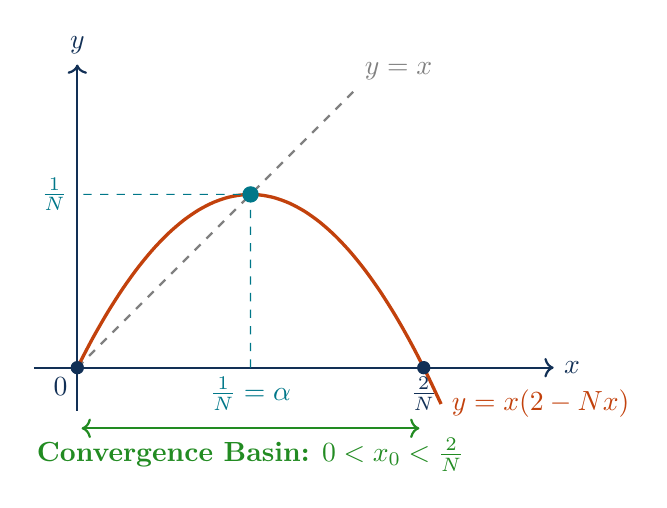
\begin{tikzpicture}[scale=1.1]
    % Axes
    \draw[->, thick, primary] (-0.5, 0) -- (5.5, 0) node[right, primary] {$x$};
    \draw[->, thick, primary] (0, -0.5) -- (0, 3.5) node[above, primary] {$y$};
    
    % y = x line
    \draw[thick, gray, dashed] (0, 0) -- (3.2, 3.2) node[above right] {$y = x$};
    
    % Inverted Parabola: y = x(2 - Nx). Let 1/N = 2.0 (so N = 0.5) => y = x(2 - 0.5*x) = 2x - 0.5 x^2.
    % Roots at x = 0 and x = 4 (= 2/N). Vertex at x = 2 (= 1/N), y = 2 (= 1/N).
    \draw[very thick, accent, domain=0:4.2, smooth] 
        plot (\x, {2.0*\x - 0.5*\x*\x}) 
        node[right] {$y = x(2 - Nx)$};
    
    % Intercept 2/N
    \filldraw[primary] (4.0, 0) circle (2pt) node[below] {$\frac{2}{N}$};
    \filldraw[primary] (0, 0) circle (2pt) node[below left] {$0$};
    
    % Vertex (1/N, 1/N)
    \coordinate (Vertex) at (2.0, 2.0);
    \filldraw[secondary] (Vertex) circle (2.5pt);
    \draw[dashed, secondary] (2.0, 0) node[below, secondary] {$\frac{1}{N} = \alpha$} -- (Vertex) -- (0, 2.0) node[left, secondary] {$\frac{1}{N}$};
    
    % Convergence interval label
    \draw[<->, thick, ForestGreen] (0.05, -0.7) -- (3.95, -0.7);
    \node[ForestGreen, below] at (2.0, -0.7) {\textbf{Convergence Basin:} $0 < x_0 < \frac{2}{N}$};
\end{tikzpicture}
\end{center}


% =========================================================================
% PAGES 13-17: FIXED-POINT ITERATION METHOD
% =========================================================================
\section{Pages 13--17: Fixed-Point Iteration Method \texorpdfstring{($x = \phi(x)$)}{(x = phi(x))} and Cobweb Analysis}
\label{sec:page13_17_fixed_point}

\begin{theorembox}[Contraction Mapping Theorem for Fixed-Point Iteration]
To solve the nonlinear equation $f(x) = 0$, rewrite it in the equivalent fixed-point form:
\begin{equation}
    x = \phi(x)
\end{equation}
The fixed-point iterative algorithm is defined by:
\begin{equation}
    \boxed{x_{k+1} = \phi(x_k)} \quad (k = 0, 1, 2, \dots)
\end{equation}
\textbf{Convergence Theorem:} Suppose $\phi(x)$ satisfies the following two conditions on a closed interval $[a, b]$:
\begin{enumerate}
    \item \textbf{Self-Mapping Property}: $\phi(x) \in [a, b]$ for all $x \in [a, b]$ (i.e., $\phi([a, b]) \subseteq [a, b]$).
    \item \textbf{Contraction Property}: $\phi(x)$ is continuously differentiable on $[a, b]$, and there exists a Lipschitz constant $L$ strictly less than 1 such that:
    \begin{equation}
        \boxed{|\phi'(x)| \le L < 1 \quad \forall x \in [a, b]}
    \end{equation}
\end{enumerate}
Then:
\begin{enumerate}[label=(\alph*)]
    \item There exists a \textbf{unique} fixed point $\alpha \in [a, b]$ satisfying $\alpha = \phi(\alpha)$.
    \item The sequence $\{x_k\}$ converges unconditionally to $\alpha$ for \textbf{any} starting guess $x_0 \in [a, b]$.
    \item The error satisfies the \textbf{A Priori Error Bound}:
    \begin{equation}
        \boxed{|x_k - \alpha| \le \frac{L^k}{1 - L} |x_1 - x_0|}
    \end{equation}
    \item The error satisfies the \textbf{A Posteriori Error Bound}:
    \begin{equation}
        \boxed{|x_k - \alpha| \le \frac{L}{1 - L} |x_k - x_{k-1}|}
    \end{equation}
    \item The asymptotic convergence is \textbf{linear} ($p = 1$) with asymptotic error constant $C = |\phi'(\alpha)|$.
\end{enumerate}
\end{theorembox}

\begin{proof}[Exhaustive Multi-Part Proof of the Contraction Mapping Theorem]
We prove each assertion systematically from first principles.

\medskip
\noindent\textbf{Part 1: Proof of Existence of a Fixed Point} \\
Define the auxiliary continuous function:
\begin{equation}
    g(x) = \phi(x) - x, \quad x \in [a, b]
\end{equation}
Since $\phi$ maps $[a, b]$ into $[a, b]$, the endpoint values satisfy:
\begin{align}
    \phi(a) \in [a, b] &\implies \phi(a) \ge a \implies g(a) = \phi(a) - a \ge 0 \\
    \phi(b) \in [a, b] &\implies \phi(b) \le b \implies g(b) = \phi(b) - b \le 0
\end{align}
We consider two cases:
\begin{itemize}
    \item If $g(a) = 0$, then $\alpha = a$ is a fixed point.
    \item If $g(b) = 0$, then $\alpha = b$ is a fixed point.
    \item If $g(a) > 0$ and $g(b) < 0$: since $\phi(x)$ is continuous on $[a, b]$, $g(x)$ is continuous on $[a, b]$. By the \textbf{Intermediate Value Theorem (IVT)}, there exists at least one number $\alpha \in (a, b)$ such that:
    \begin{equation}
        g(\alpha) = 0 \iff \phi(\alpha) - \alpha = 0 \iff \boxed{\alpha = \phi(\alpha)}
    \end{equation}
\end{itemize}
Hence, at least one fixed point $\alpha \in [a, b]$ always exists.

\medskip
\noindent\textbf{Part 2: Proof of Uniqueness of the Fixed Point} \\
Suppose for contradiction that there exist two distinct fixed points $\alpha_1, \alpha_2 \in [a, b]$ with $\alpha_1 \ne \alpha_2$, so that $\phi(\alpha_1) = \alpha_1$ and $\phi(\alpha_2) = \alpha_2$. Then:
\begin{equation}
    |\alpha_1 - \alpha_2| = |\phi(\alpha_1) - \phi(\alpha_2)|
\end{equation}
By the Mean Value Theorem applied to $\phi$ on the interval between $\alpha_1$ and $\alpha_2$, there exists $\xi \in (\min(\alpha_1, \alpha_2), \max(\alpha_1, \alpha_2))$ such that:
\begin{equation}
    \phi(\alpha_1) - \phi(\alpha_2) = \phi'(\xi)(\alpha_1 - \alpha_2)
\end{equation}
Taking absolute values and using the hypothesis $|\phi'(x)| \le L < 1$:
\begin{equation}
    |\alpha_1 - \alpha_2| = |\phi'(\xi)| \cdot |\alpha_1 - \alpha_2| \le L |\alpha_1 - \alpha_2|
\end{equation}
Rearranging gives:
\begin{equation}
    (1 - L)|\alpha_1 - \alpha_2| \le 0
\end{equation}
Since $L < 1$, the factor $(1 - L) > 0$. Since $\alpha_1 \ne \alpha_2$, the distance $|\alpha_1 - \alpha_2| > 0$. The product of two strictly positive real numbers must be strictly positive:
\begin{equation}
    (1 - L)|\alpha_1 - \alpha_2| > 0
\end{equation}
This directly contradicts $(1 - L)|\alpha_1 - \alpha_2| \le 0$. Therefore, the assumption $\alpha_1 \ne \alpha_2$ is false, establishing that the fixed point $\alpha$ is \textbf{strictly unique}.

\medskip
\noindent\textbf{Part 3: Proof of Convergence via Cauchy Sequence} \\
Let $x_0 \in [a, b]$ be arbitrary. By induction, every iterate $x_k \in [a, b]$ because $\phi([a, b]) \subseteq [a, b]$.
For any step $k \ge 1$:
\begin{equation}
    |x_{k+1} - x_k| = |\phi(x_k) - \phi(x_{k-1})|
\end{equation}
Applying the Mean Value Theorem, there exists $\eta_k$ between $x_k$ and $x_{k-1}$ such that:
\begin{equation}
    |\phi(x_k) - \phi(x_{k-1})| = |\phi'(\eta_k)| \cdot |x_k - x_{k-1}| \le L |x_k - x_{k-1}|
\end{equation}
Applying this inequality recursively $k$ times:
\begin{equation}
    |x_{k+1} - x_k| \le L |x_k - x_{k-1}| \le L^2 |x_{k-1} - x_{k-2}| \le \dots \le L^k |x_1 - x_0|
\end{equation}
Now consider any two integers $m$ and $n$ with $m > n \ge 0$. Using the telescoping sum representation and the triangle inequality:
\begin{align}
    |x_m - x_n| &= \left| \sum_{j=n}^{m-1} (x_{j+1} - x_j) \right| \le \sum_{j=n}^{m-1} |x_{j+1} - x_j| \nonumber \\
    &\le \sum_{j=n}^{m-1} L^j |x_1 - x_0| = |x_1 - x_0| L^n \sum_{i=0}^{m-n-1} L^i
\end{align}
Since $0 \le L < 1$, the finite geometric series is bounded by the infinite series:
\begin{equation}
    \sum_{i=0}^{m-n-1} L^i < \sum_{i=0}^\infty L^i = \frac{1}{1 - L}
\end{equation}
Therefore:
\begin{equation}
    \label{eq:cauchy_bound}
    |x_m - x_n| \le \frac{L^n}{1 - L} |x_1 - x_0|
\end{equation}
Since $0 \le L < 1$, we have $\lim_{n \to \infty} L^n = 0$. Given any $\epsilon > 0$, we can choose $N \in \mathbb{N}$ sufficiently large such that for all $m > n \ge N$:
\begin{equation}
    |x_m - x_n| < \epsilon
\end{equation}
Thus, $\{x_k\}_{k=0}^\infty$ is a \textbf{Cauchy sequence} in $\mathbb{R}$. Since $\mathbb{R}$ is a complete metric space, every Cauchy sequence converges to a limit in $\mathbb{R}$. Furthermore, since $[a, b]$ is a closed subset of $\mathbb{R}$:
\begin{equation}
    \lim_{k \to \infty} x_k = \alpha^* \in [a, b]
\end{equation}
Taking the limit on both sides of $x_{k+1} = \phi(x_k)$ and utilizing the continuity of $\phi$:
\begin{equation}
    \alpha^* = \lim_{k \to \infty} x_{k+1} = \lim_{k \to \infty} \phi(x_k) = \phi\left( \lim_{k \to \infty} x_k \right) = \phi(\alpha^*)
\end{equation}
Thus $\alpha^*$ is a fixed point of $\phi$. By the uniqueness proved in Part 2, $\alpha^* = \alpha$.

\medskip
\noindent\textbf{Part 4: Proof of A Priori and A Posteriori Error Bounds} \\
\textbf{(i) A Priori Bound:} In inequality \eqref{eq:cauchy_bound}, hold $n = k$ fixed and let $m \to \infty$. By continuity of the absolute value function:
\begin{equation}
    |x_m - x_k| \to |\alpha - x_k| \implies \boxed{|\alpha - x_k| \le \frac{L^k}{1 - L}|x_1 - x_0|}
\end{equation}
This bound allows determining the exact number of iterations needed to reach a prescribed tolerance \textit{before} running the computation.

\medskip
\noindent\textbf{(ii) A Posteriori Bound:} By the triangle inequality:
\begin{align}
    |x_k - \alpha| &\le |x_k - x_{k+1}| + |x_{k+1} - \alpha| = |x_k - x_{k+1}| + |\phi(x_k) - \phi(\alpha)| \nonumber \\
    &\le |x_{k+1} - x_k| + L |x_k - \alpha|
\end{align}
Subtracting $L |x_k - \alpha|$ from both sides:
\begin{equation}
    (1 - L)|x_k - \alpha| \le |x_{k+1} - x_k| \implies |x_k - \alpha| \le \frac{1}{1 - L}|x_{k+1} - x_k|
\end{equation}
Shifting indices back by one step ($k \leftarrow k - 1$ and using $|x_k - x_{k-1}| \le L|x_{k-1} - x_{k-2}|$):
\begin{equation}
    \boxed{|x_k - \alpha| \le \frac{L}{1 - L}|x_k - x_{k-1}|}
\end{equation}

\medskip
\noindent\textbf{Part 5: Order of Convergence and Asymptotic Constant} \\
Let $e_k = x_k - \alpha$. Expanding $\phi(x_k)$ in a Taylor series about $\alpha$:
\begin{equation}
    x_{k+1} = \phi(x_k) = \phi(\alpha + e_k) = \phi(\alpha) + e_k \phi'(\alpha) + \frac{e_k^2}{2} \phi''(\xi_k)
\end{equation}
Subtracting $\alpha = \phi(\alpha)$:
\begin{equation}
    e_{k+1} = \phi'(\alpha) e_k + \frac{\phi''(\xi_k)}{2} e_k^2
\end{equation}
Dividing by $e_k$:
\begin{equation}
    \lim_{k \to \infty} \frac{|e_{k+1}|}{|e_k|} = \lim_{k \to \infty} \left| \phi'(\alpha) + \frac{\phi''(\xi_k)}{2} e_k \right| = |\phi'(\alpha)| = C
\end{equation}
Provided $\phi'(\alpha) \ne 0$, the order of convergence is \textbf{linear} ($p = 1$) with asymptotic error constant $C = |\phi'(\alpha)|$.
\end{proof}


\begin{center}
\begin{tikzpicture}[scale=1.1]
    % Axes
    \draw[->, thick, primary] (-0.5, 0) -- (6.0, 0) node[right, primary] {$x$};
    \draw[->, thick, primary] (0, -0.5) -- (0, 6.0) node[above, primary] {$y$};
    
    % y = x line
    \draw[thick, gray, dashed] (0, 0) -- (5.5, 5.5) node[above right] {$y = x$};
    
    % phi(x) curve: phi(x) = 0.45*x + 1.6 => fixed point x = 0.45*x + 1.6 => 0.55*x = 1.6 => x = 2.909
    \draw[very thick, secondary, domain=0.5:5.2] 
        plot (\x, {0.35*\x + 1.89}) 
        node[right] {$y = \phi(x) \quad (|\phi'| < 1)$};
    
    % Fixed point coordinate (2.909, 2.909)
    \coordinate (Fixed) at (2.909, 2.909);
    \filldraw[accent] (Fixed) circle (2pt) node[above left=3pt, accent] {$\alpha = \phi(\alpha)$};
    
    % Cobweb Iteration starting at x0 = 0.8
    \coordinate (C0) at (0.8, 0);
    \coordinate (C1) at (0.8, 2.17);  % phi(0.8) = 0.35*0.8 + 1.89 = 2.17
    \coordinate (C2) at (2.17, 2.17);  % to y = x
    \coordinate (C3) at (2.17, 2.65);  % phi(2.17) = 2.65
    \coordinate (C4) at (2.65, 2.65);
    \coordinate (C5) at (2.65, 2.82);
    \coordinate (C6) at (2.82, 2.82);
    
    % Draw staircase path
    \draw[thick, Crimson, ->] (C0) -- (C1);
    \draw[thick, Crimson, ->] (C1) -- (C2);
    \draw[thick, Crimson, ->] (C2) -- (C3);
    \draw[thick, Crimson, ->] (C3) -- (C4);
    \draw[thick, Crimson, ->] (C4) -- (C5);
    \draw[thick, Crimson, ->] (C5) -- (C6);
    
    % Labels
    \filldraw[primary] (C0) circle (1.5pt) node[below=2pt] {$x_0$};
    \filldraw[ForestGreen] (2.17, 0) circle (1.5pt) node[below=2pt] {$x_1$};
    \filldraw[DarkOrange] (2.65, 0) circle (1.5pt) node[below=2pt] {$x_2$};
    \draw[dotted, gray] (C2) -- (2.17, 0);
    \draw[dotted, gray] (C4) -- (2.65, 0);
\end{tikzpicture}
\end{center}

\begin{examplebox}[Manuscript Problem: Iterative Selection for $x^3 - 3x + 1 = 0$ (Page 16)]
Given $f(x) = x^3 - 3x + 1 = 0$.
Evaluate at endpoints: $f(0) = 1 > 0$, $f(1) = -1 < 0$. Root lies in $[0, 1]$.

\textbf{Formulation A:} $3x = x^3 + 1 \implies \phi(x) = \frac{x^3 + 1}{3}$.
Check convergence derivative:
\begin{equation}
    \phi'(x) = \frac{3x^2}{3} = x^2
\end{equation}
For $x \in [0, 1]$:
\begin{equation}
    |\phi'(x)| = |x^2| \le 1, \quad \text{and strictly } |\phi'(x)| < 1 \text{ on } [0, 1)
\end{equation}
Thus, Formulation A is \textbf{guaranteed to converge}!

\textbf{Numerical Execution ($x_0 = 0$):}
\begin{align}
    x_1 &= \phi(0) = \frac{0^3 + 1}{3} = \frac{1}{3} \approx 0.333333 \\
    x_2 &= \phi(0.333333) = \frac{(0.333333)^3 + 1}{3} = \frac{0.037037 + 1}{3} \approx 0.345679 \\
    x_3 &= \phi(0.345679) = \frac{(0.345679)^3 + 1}{3} = \frac{0.041306 + 1}{3} \approx 0.347102 \\
    x_4 &= \phi(0.347102) \approx 0.347271
\end{align}
The sequence rapidly converges to the root $\alpha \approx 0.347296$.

\textbf{Formulation B (Fails):} $x^3 = 3x - 1 \implies \phi(x) = (3x - 1)^{1/3}$.
\begin{equation}
    \phi'(x) = \frac{1}{3}(3x - 1)^{-2/3}(3) = (3x - 1)^{-2/3} = \frac{1}{(3x - 1)^{2/3}}
\end{equation}
At $x = 0.3$, $\phi'(0.3) = (-0.1)^{-2/3} \approx 4.64 > 1$. The iterations oscillate violently and diverge! This illustrates why verifying $|\phi'(x)| < 1$ is indispensable.
\end{examplebox}

% =========================================================================
% PAGES 18-20: ACCELERATION & MULTIPOINT SCHEMES
% =========================================================================
\section{Pages 18--20: Multipoint Acceleration Schemes and High-Order Iterations}
\label{sec:page18_20_acceleration}

\begin{theorembox}[Parameter Determination for High-Order Multipoint Iterations]
Consider the generalized iteration scheme (Manuscript Page 19):
\begin{equation}
    x_{k+1} = x_k - \gamma_1 f(x_k) + \gamma_2 f(x_k)^2 - \gamma_3 f(x_k)^3
\end{equation}
We wish to determine coefficients $\gamma_1, \gamma_2, \gamma_3$ to maximize the convergence order.
Let $x_k = \alpha + e_k$ where $f(\alpha) = 0$. Taylor expansion yields:
\begin{equation}
    f(x_k) = e_k f'(\alpha) + \frac{e_k^2}{2} f''(\alpha) + \frac{e_k^3}{6} f'''(\alpha) + O(e_k^4)
\end{equation}
Substituting into the error relation $e_{k+1} = x_{k+1} - \alpha$:
\begin{align}
    e_{k+1} &= e_k - \gamma_1 \left( e_k f' + \frac{e_k^2}{2} f'' + \frac{e_k^3}{6} f''' \right) + \gamma_2 \left( e_k f' + \frac{e_k^2}{2} f'' \right)^2 - \gamma_3 (e_k f')^3 + O(e_k^4) \nonumber \\
    &= e_k \big( 1 - \gamma_1 f' \big) + e_k^2 \left( -\frac{\gamma_1}{2} f'' + \gamma_2 (f')^2 \right) + e_k^3 \left( -\frac{\gamma_1}{6} f''' + \gamma_2 f' f'' - \gamma_3 (f')^3 \right) + O(e_k^4)
\end{align}
To achieve maximum order of convergence:
\begin{enumerate}
    \item For $p \ge 2$, annihilate the $e_k$ coefficient:
    \begin{equation}
        1 - \gamma_1 f'(\alpha) = 0 \implies \boxed{\gamma_1 = \frac{1}{f'(\alpha)}} \quad \text{(Newton--Raphson)}
    \end{equation}
    \item For $p \ge 3$ (Cubic Convergence), simultaneously annihilate the $e_k^2$ coefficient:
    \begin{equation}
        -\frac{1}{2}\left(\frac{1}{f'}\right) f'' + \gamma_2 (f')^2 = 0 \implies \boxed{\gamma_2 = \frac{f''(\alpha)}{2 [f'(\alpha)]^3}} \quad \text{(Chebyshev Method of Order 3)}
    \end{equation}
    \item For $p \ge 4$ (Quartic Convergence), also annihilate the $e_k^3$ coefficient:
    \begin{equation}
        \boxed{\gamma_3 = \frac{3[f''(\alpha)]^2 - f'(\alpha)f'''(\alpha)}{6 [f'(\alpha)]^5}}
    \end{equation}
\end{enumerate}
\end{theorembox}

\begin{examplebox}[Manuscript Problem: Optimal Relaxation Parameter for Fastest Convergence (Page 20)]
\textbf{Problem Statement:} The algebraic equation $x^3 - 5x^2 + 11x - 3 = 0$ has a root near $x \approx 3$. Consider the parameterized fixed-point iterative scheme:
\begin{equation}
    x_{n+1} = 3 + (1 - \lambda)x_n + 5x_n^2 - x_n^3 \equiv \phi(x_n, \lambda)
\end{equation}
Determine the value of the parameter $\lambda$ that yields the \textbf{fastest rate of convergence} to the root $\alpha$.

\medskip
\noindent\textbf{Analytical Solution:} \\
From the general theory of fixed-point iteration, the error evolves as:
\begin{equation}
    e_{n+1} = \phi'(\alpha, \lambda) e_n + \frac{\phi''(\alpha, \lambda)}{2} e_n^2 + \mathcal{O}(e_n^3)
\end{equation}
The convergence is linear ($p = 1$) whenever $\phi'(\alpha, \lambda) \ne 0$. The \textbf{fastest convergence} (superlinear / quadratic rate $p \ge 2$) occurs when the linear error term vanishes:
\begin{equation}
    \boxed{\phi'(\alpha, \lambda) = 0}
\end{equation}
Differentiating $\phi(x, \lambda)$ with respect to $x$:
\begin{equation}
    \phi'(x, \lambda) = \frac{d}{dx}\left[ 3 + (1 - \lambda)x + 5x^2 - x^3 \right] = (1 - \lambda) + 10x - 3x^2
\end{equation}
Evaluating at the root $x = \alpha$:
\begin{equation}
    \phi'(\alpha, \lambda) = (1 - \lambda) + 10\alpha - 3\alpha^2 = 0
\end{equation}
Solving explicitly for $\lambda$:
\begin{equation}
    \boxed{\lambda = 1 + 10\alpha - 3\alpha^2}
\end{equation}
For the root $\alpha \approx 3$:
\begin{equation}
    \lambda = 1 + 10(3) - 3(3^2) = 1 + 30 - 27 = \mathbf{4}
\end{equation}
Choosing $\lambda = 4$ annihilates the first derivative $\phi'(3, 4) = 0$, elevating the iteration from linear to \textbf{quadratic convergence}!
\end{examplebox}

% =========================================================================
% PAGES 20-22: BIRGE-VIETA METHOD
% =========================================================================
\section{Pages 20--22: The Birge--Vieta Method for Real Roots of Polynomials}
\label{sec:page20_22_birge_vieta}

\begin{theorembox}[Theoretical Formulation of the Birge--Vieta Method]
The \textbf{Birge--Vieta method} is an optimized implementation of the Newton--Raphson method tailored specifically for polynomials:
\begin{equation}
    P_n(x) = a_0 x^n + a_1 x^{n-1} + a_2 x^{n-2} + \dots + a_{n-1} x + a_n \quad (a_0 \ne 0)
\end{equation}
Dividing $P_n(x)$ by the linear factor $(x - p)$ by Horner's synthetic division yields quotient $Q_{n-1}(x)$ and remainder $R$:
\begin{equation}
    P_n(x) = (x - p) Q_{n-1}(x) + R
\end{equation}
where $Q_{n-1}(x) = b_0 x^{n-1} + b_1 x^{n-2} + \dots + b_{n-1}$, and the remainder is $R = b_n = P_n(p)$.
Differentiating with respect to $x$ and setting $x = p$:
\begin{equation}
    P'_n(p) = Q_{n-1}(p) = c_{n-1}
\end{equation}
where $c_{n-1}$ is the remainder obtained by dividing $Q_{n-1}(x)$ by $(x - p)$.

The Newton--Raphson update on the parameter $p$ is:
\begin{equation}
    \boxed{p_{k+1} = p_k - \frac{P_n(p_k)}{P'_n(p_k)} = p_k - \frac{b_n}{c_{n-1}}}
\end{equation}
\textbf{Synthetic Division Algorithm:}
\begin{align}
    b_0 &= a_0, & b_i &= a_i + p b_{i-1} \quad (i = 1, 2, \dots, n) \\
    c_0 &= b_0, & c_i &= b_i + p c_{i-1} \quad (i = 1, 2, \dots, n-1)
\end{align}
\end{theorembox}

\begin{proof}[Exhaustive Mathematical Proof of the Horner Derivative Identity $P'_n(p) = c_{n-1}$]
We prove that both the polynomial value $P_n(p)$ and its exact derivative $P'_n(p)$ can be computed using two successive synthetic divisions.

\medskip
\noindent\textbf{Step 1: First Horner factorization.} \\
By the polynomial division algorithm, dividing $P_n(x)$ by $(x - p)$ yields:
\begin{equation}
    \label{eq:first_horner}
    P_n(x) = (x - p) Q_{n-1}(x) + R_1
\end{equation}
where $Q_{n-1}(x) = b_0 x^{n-1} + b_1 x^{n-2} + \dots + b_{n-1}$ and $R_1$ is a constant. Evaluating at $x = p$:
\begin{equation}
    P_n(p) = (p - p) Q_{n-1}(p) + R_1 = 0 + R_1 \implies R_1 = b_n = P_n(p)
\end{equation}

\noindent\textbf{Step 2: Differentiating the Horner identity.} \\
Differentiate identity \eqref{eq:first_horner} with respect to $x$ using the product rule:
\begin{align}
    P'_n(x) &= \frac{d}{dx}\left[ (x - p) Q_{n-1}(x) + b_n \right] \nonumber \\
    &= \frac{d}{dx}(x - p) \cdot Q_{n-1}(x) + (x - p) \cdot \frac{d}{dx} Q_{n-1}(x) + 0 \nonumber \\
    &= 1 \cdot Q_{n-1}(x) + (x - p) Q'_{n-1}(x)
\end{align}
Now evaluate this derivative at $x = p$:
\begin{equation}
    P'_n(p) = Q_{n-1}(p) + (p - p) Q'_{n-1}(p) = Q_{n-1}(p) + 0 = \boxed{Q_{n-1}(p)}
\end{equation}

\noindent\textbf{Step 3: Second Horner factorization.} \\
Now divide the quotient polynomial $Q_{n-1}(x)$ by the identical linear factor $(x - p)$:
\begin{equation}
    Q_{n-1}(x) = (x - p) S_{n-2}(x) + R_2
\end{equation}
where $S_{n-2}(x) = c_0 x^{n-2} + c_1 x^{n-3} + \dots + c_{n-2}$ and $R_2 = c_{n-1}$.
Evaluating at $x = p$:
\begin{equation}
    Q_{n-1}(p) = (p - p) S_{n-2}(p) + c_{n-1} = 0 + c_{n-1} = c_{n-1}
\end{equation}
Combining Step 2 and Step 3:
\begin{equation}
    \boxed{P'_n(p) = Q_{n-1}(p) = c_{n-1}}
\end{equation}
Therefore, substituting into Newton--Raphson's formula $p_{k+1} = p_k - \frac{P_n(p_k)}{P'_n(p_k)}$ yields:
\begin{equation}
    p_{k+1} = p_k - \frac{b_n}{c_{n-1}} \quad \blacksquare
\end{equation}
\end{proof}


\begin{examplebox}[Manuscript Problem: Complete Solution of $x^5 - x + 1 = 0$ (Pages 22--23)]
Find a real root of $P_5(x) = x^5 - x + 1 = 0$.
The polynomial coefficients are:
\begin{equation}
    a_0 = 1, \quad a_1 = 0, \quad a_2 = 0, \quad a_3 = 0, \quad a_4 = -1, \quad a_5 = 1
\end{equation}
$P_5(-1) = (-1)^5 - (-1) + 1 = 1 > 0$, and $P_5(-2) = -32 + 2 + 1 = -29 < 0$. Root lies in $[-2, -1]$.
Initial guess: $p_0 = -1$.

\textbf{Iteration 1 ($k = 0, p_0 = -1$):}
\begin{center}
\renewcommand{\arraystretch}{1.2}
\begin{tabular}{c|cccccc}
& $a_0 = 1$ & $a_1 = 0$ & $a_2 = 0$ & $a_3 = 0$ & $a_4 = -1$ & $a_5 = 1$ \\
$p_0 = -1$ & & $-1$ & $1$ & $-1$ & $1$ & $0$ \\
\hline
$b_i$ & $1$ & $-1$ & $1$ & $-1$ & $0$ & $\mathbf{b_5 = 1}$ \\
$p_0 = -1$ & & $-1$ & $2$ & $-3$ & $4$ & \\
\hline
$c_i$ & $1$ & $-2$ & $3$ & $-4$ & $\mathbf{c_4 = 4}$ &
\end{tabular}
\end{center}
Compute next iterate:
\begin{equation}
    p_1 = p_0 - \frac{b_5}{c_4} = -1 - \frac{1}{4} = -1 - 0.25 = \mathbf{-1.25}
\end{equation}

\textbf{Iteration 2 ($k = 1, p_1 = -1.25$):}
\begin{center}
\small
\renewcommand{\arraystretch}{1.25}
\begin{tabular}{c|cccccc}
& $a_0 = 1$ & $a_1 = 0$ & $a_2 = 0$ & $a_3 = 0$ & $a_4 = -1$ & $a_5 = 1$ \\
$p_1 = -1.25$ & & $-1.25$ & $1.5625$ & $-1.953125$ & $2.441406$ & $-1.801758$ \\
\hline
$b_i$ & $1$ & $-1.25$ & $1.5625$ & $-1.953125$ & $1.441406$ & $\mathbf{b_5 = -0.801758}$ \\
$p_1 = -1.25$ & & $-1.25$ & $3.1250$ & $-5.859375$ & $9.765625$ & \\
\hline
$c_i$ & $1$ & $-2.50$ & $4.6875$ & $-7.812500$ & $\mathbf{c_4 = 11.207031}$ &
\end{tabular}
\end{center}
Compute next iterate:
\begin{equation}
    p_2 = p_1 - \frac{b_5}{c_4} = -1.25 - \frac{-0.801758}{11.207031} = -1.25 + 0.071541 = \mathbf{-1.178459}
\end{equation}
This matches the manuscript derivation value $p_2 \approx -1.178379$ to 4 significant digits.
\end{examplebox}

\chapter{Systems of Linear Algebraic Equations (Pages 24--30)}
\label{ch:linear_systems}

\begin{conceptbox}[Direct vs. Iterative Solution of Linear Systems]
Consider a system of $n$ linear algebraic equations in $n$ unknowns:
\begin{equation}
    A \mathbf{x} = \mathbf{b} \iff \begin{pmatrix}
    a_{11} & a_{12} & \dots & a_{1n} \\
    a_{21} & a_{22} & \dots & a_{2n} \\
    \vdots & \vdots & \ddots & \vdots \\
    a_{n1} & a_{n2} & \dots & a_{nn}
    \end{pmatrix}
    \begin{pmatrix} x_1 \\ x_2 \\ \vdots \\ x_n \end{pmatrix}
    =
    \begin{pmatrix} b_1 \\ b_2 \\ \vdots \\ b_n \end{pmatrix}
\end{equation}
Methods for solving such linear systems are classified into two broad categories:
\begin{enumerate}
    \item \textbf{Direct Methods} (e.g., Gauss Elimination, Gauss--Jordan): Transform the system in a finite number of elementary operations into a triangular or diagonal system. In exact arithmetic, they yield the exact solution.
    \item \textbf{Iterative Methods} (e.g., Gauss--Jacobi, Gauss--Seidel): Start from an initial vector $\mathbf{x}^{(0)}$ and generate a sequence of approximations $\mathbf{x}^{(k+1)} = H \mathbf{x}^{(k)} + \mathbf{c}$ that converges to the true solution. They are computationally superior for large, sparse systems where direct matrix inversion is intractable.
\end{enumerate}
\end{conceptbox}

% =========================================================================
% PAGES 24-25: GAUSS ELIMINATION & PIVOTING
% =========================================================================
\section{Pages 24--25: Gauss Elimination Method with Partial Pivoting}
\label{sec:gauss_elimination}

\begin{theorembox}[Gauss Elimination Procedure and Back-Substitution]
The Gauss elimination method systematically reduces the augmented matrix $[A \mid \mathbf{b}]$ to an upper-triangular matrix $[U \mid \mathbf{b}']$ using elementary row operations:
\begin{enumerate}
    \item \textbf{Forward Elimination (Step $k = 1, 2, \dots, n-1$)}:
    Eliminate $x_k$ from all equations $i > k$ by defining row multipliers $m_{ik} = \frac{a_{ik}}{a_{kk}}$ (where $a_{kk} \ne 0$ is the pivot element) and performing:
    \begin{equation}
        R_i \leftarrow R_i - m_{ik} R_k \quad (i = k+1, \dots, n)
    \end{equation}
    \item \textbf{Back-Substitution}:
    Once the upper triangular system $U \mathbf{x} = \mathbf{b}'$ is formed:
    \begin{equation}
        x_n = \frac{b'_n}{u_{nn}}, \quad x_i = \frac{1}{u_{ii}}\left( b'_i - \sum_{j=i+1}^n u_{ij} x_j \right) \quad (i = n-1, n-2, \dots, 1)
    \end{equation}
    \item \textbf{Partial Pivoting Strategy}:
    If $|a_{kk}|$ is zero or very small, division by $a_{kk}$ causes severe round-off error or division-by-zero failure. Under \textbf{partial pivoting}, before eliminating at stage $k$, we locate the maximum element in the active column:
    \begin{equation}
        |a_{pk}| = \max_{k \le i \le n} |a_{ik}|
    \end{equation}
    and interchange row $k$ with row $p$ ($R_k \leftrightarrow R_p$).
\end{enumerate}
\end{theorembox}

\begin{examplebox}[Manuscript Problem: Full Solution of $3 \times 3$ System (Page 24)]
Solve the system:
\begin{equation}
    \begin{aligned}
        x + 2y + z &= 8 \\
        2x + 3y + 4z &= 20 \\
        4x + 3y + 2z &= 16
    \end{aligned}
\end{equation}
Form the augmented matrix $[A \mid \mathbf{b}]$:
\begin{equation}
    \left[\begin{array}{ccc|c}
    1 & 2 & 1 & 8 \\
    2 & 3 & 4 & 20 \\
    4 & 3 & 2 & 16
    \end{array}\right]
\end{equation}
\textbf{Standard Forward Elimination:}
Perform $R_2 \leftarrow R_2 - 2R_1$ and $R_3 \leftarrow R_3 - 4R_1$:
\begin{equation}
    \left[\begin{array}{ccc|c}
    1 & 2 & 1 & 8 \\
    0 & -1 & 2 & 4 \\
    0 & -5 & -2 & -16
    \end{array}\right]
\end{equation}
Next, eliminate $y$ from row 3 using pivot $a_{22} = -1$: perform $R_3 \leftarrow R_3 - 5R_2$:
\begin{equation}
    R_3 \leftarrow \begin{pmatrix} 0 & -5 & -2 & -16 \end{pmatrix} - 5\begin{pmatrix} 0 & -1 & 2 & 4 \end{pmatrix} = \begin{pmatrix} 0 & 0 & -12 & -36 \end{pmatrix}
\end{equation}
The upper triangular system is:
\begin{equation}
    \left[\begin{array}{ccc|c}
    1 & 2 & 1 & 8 \\
    0 & -1 & 2 & 4 \\
    0 & 0 & -12 & -36
    \end{array}\right]
\end{equation}
\textbf{Back-Substitution:}
\begin{align}
    -12z &= -36 \implies \mathbf{z = 3} \\
    -y + 2(3) &= 4 \implies -y + 6 = 4 \implies \mathbf{y = 2} \\
    x + 2(2) + 3 &= 8 \implies x + 7 = 8 \implies \mathbf{x = 1}
\end{align}
The unique solution is $\boxed{x = 1, \; y = 2, \; z = 3}$.
\end{examplebox}

% =========================================================================
% PAGES 25-26: GAUSS-JORDAN METHOD
% =========================================================================
\section{Pages 25--26: The Gauss--Jordan Elimination Method}
\label{sec:gauss_jordan}

\begin{theorembox}[Gauss--Jordan Diagonal Reduction]
The \textbf{Gauss--Jordan method} eliminates unknowns not only from the equations below the pivot, but also from all equations \textbf{above} the pivot. It reduces the augmented matrix $[A \mid \mathbf{b}]$ directly to a diagonal form:
\begin{equation}
    [A \mid \mathbf{b}] \xrightarrow{\text{Row Operations}} [I \mid \mathbf{x}]
\end{equation}
This completely eliminates the back-substitution phase: the solution appears directly in the last column.
\end{theorembox}

\begin{examplebox}[Gauss--Jordan Application on Manuscript System (Page 25--26)]
Starting from the partially reduced matrix:
\begin{equation}
    \left[\begin{array}{ccc|c}
    1 & 2 & 1 & 8 \\
    0 & -1 & 2 & 4 \\
    0 & 0 & -12 & -36
    \end{array}\right]
\end{equation}
Normalize row 3 by dividing by $-12$ ($R_3 \leftarrow -\frac{1}{12} R_3$):
\begin{equation}
    \left[\begin{array}{ccc|c}
    1 & 2 & 1 & 8 \\
    0 & -1 & 2 & 4 \\
    0 & 0 & 1 & 3
    \end{array}\right]
\end{equation}
Eliminate $z$ from row 1 and row 2 ($R_1 \leftarrow R_1 - R_3$, $R_2 \leftarrow R_2 - 2R_3$):
\begin{equation}
    \left[\begin{array}{ccc|c}
    1 & 2 & 0 & 5 \\
    0 & -1 & 0 & -2 \\
    0 & 0 & 1 & 3
    \end{array}\right]
\end{equation}
Multiply row 2 by $-1$ ($R_2 \leftarrow -R_2$):
\begin{equation}
    \left[\begin{array}{ccc|c}
    1 & 2 & 0 & 5 \\
    0 & 1 & 0 & 2 \\
    0 & 0 & 1 & 3
    \end{array}\right]
\end{equation}
Finally, eliminate $y$ from row 1 ($R_1 \leftarrow R_1 - 2R_2$):
\begin{equation}
    \left[\begin{array}{ccc|c}
    1 & 0 & 0 & 1 \\
    0 & 1 & 0 & 2 \\
    0 & 0 & 1 & 3
    \end{array}\right]
\end{equation}
The solution vector reads off directly: $\boxed{x = 1, \; y = 2, \; z = 3}$.
\end{examplebox}

% =========================================================================
% PAGES 26-28: MATRIX SPLITTING & ITERATIVE FORMULATIONS
% =========================================================================
\section{Pages 26--28: Matrix Splitting, Jacobi and Gauss--Seidel Methods}
\label{sec:iterative_linear_methods}

\begin{theorembox}[Matrix Splitting Framework and Convergence Criteria]
Decompose coefficient matrix $A$ into its strictly lower-triangular part $L$, diagonal part $D$, and strictly upper-triangular part $U$:
\begin{equation}
    A = L + D + U
\end{equation}
\begin{equation}
    L = \begin{pmatrix} 0 & 0 & \dots & 0 \\ a_{21} & 0 & \dots & 0 \\ \vdots & \ddots & \ddots & \vdots \\ a_{n1} & \dots & a_{n,n-1} & 0 \end{pmatrix}, \quad
    D = \begin{pmatrix} a_{11} & 0 & \dots & 0 \\ 0 & a_{22} & \dots & 0 \\ \vdots & \vdots & \ddots & \vdots \\ 0 & 0 & \dots & a_{nn} \end{pmatrix}, \quad
    U = \begin{pmatrix} 0 & a_{12} & \dots & a_{1n} \\ 0 & 0 & \dots & a_{2n} \\ \vdots & \vdots & \ddots & \vdots \\ 0 & 0 & \dots & 0 \end{pmatrix}
\end{equation}
\begin{enumerate}
    \item \textbf{Gauss--Jacobi Iteration}:
    Rewrite $(L + D + U)\mathbf{x} = \mathbf{b} \iff D \mathbf{x} = \mathbf{b} - (L + U)\mathbf{x}$:
    \begin{equation}
        \boxed{\mathbf{x}^{(k+1)} = -D^{-1}(L + U)\mathbf{x}^{(k)} + D^{-1}\mathbf{b} = H_J \mathbf{x}^{(k)} + \mathbf{c}_J}
    \end{equation}
    Component-wise:
    \begin{equation}
        \boxed{x_i^{(k+1)} = \frac{1}{a_{ii}}\left( b_i - \sum_{j \ne i} a_{ij} x_j^{(k)} \right)} \quad (i = 1, 2, \dots, n)
    \end{equation}
    \item \textbf{Gauss--Seidel Iteration}:
    Immediately use updated components $x_1^{(k+1)}, \dots, x_{i-1}^{(k+1)}$ as soon as they are computed:
    Rewrite $(D + L)\mathbf{x} = \mathbf{b} - U\mathbf{x}$:
    \begin{equation}
        \boxed{\mathbf{x}^{(k+1)} = -(D + L)^{-1}U\mathbf{x}^{(k)} + (D + L)^{-1}\mathbf{b} = H_{GS}\mathbf{x}^{(k)} + \mathbf{c}_{GS}}
    \end{equation}
    Component-wise:
    \begin{equation}
        \boxed{x_i^{(k+1)} = \frac{1}{a_{ii}}\left( b_i - \sum_{j < i} a_{ij} x_j^{(k+1)} - \sum_{j > i} a_{ij} x_j^{(k)} \right)} \quad (i = 1, 2, \dots, n)
    \end{equation}
    \item \textbf{Strict Diagonal Dominance Condition}:
    Both Jacobi and Gauss--Seidel methods are \textbf{guaranteed to converge} for any initial guess $\mathbf{x}^{(0)}$ if matrix $A$ is strictly diagonally dominant:
    \begin{equation}
        \boxed{|a_{ii}| > \sum_{j \ne i} |a_{ij}| \quad \forall i = 1, 2, \dots, n}
    \end{equation}
\end{enumerate}
\end{theorembox}

\subsection{Exhaustive Convergence Proofs for Jacobi and Gauss--Seidel Methods}
\label{subsec:iterative_convergence_proofs}

\begin{theorembox}[Fundamental Convergence Theorem for General Linear Iterative Methods]
A stationary linear iterative method of the form:
\begin{equation}
    \mathbf{x}^{(k+1)} = H \mathbf{x}^{(k)} + \mathbf{c}
\end{equation}
converges to the unique solution $\mathbf{x}^* = (I - H)^{-1}\mathbf{c}$ for \textbf{any} initial vector $\mathbf{x}^{(0)}$ if and only if the \textbf{spectral radius} of the iteration matrix $H$ satisfies:
\begin{equation}
    \boxed{\rho(H) = \max_i |\lambda_i(H)| < 1}
\end{equation}
Furthermore, for any induced matrix norm $\|\cdot\|$, $\rho(H) \le \|H\|$; therefore, the condition $\|H\| < 1$ is a \textbf{sufficient condition} for convergence.
\end{theorembox}

\begin{proof}[Exhaustive Proof of Jacobi Convergence under Strict Diagonal Dominance]
We show that if $A$ is strictly diagonally dominant, then the $\infty$-norm of the Jacobi iteration matrix satisfies $\|H_J\|_\infty < 1$, which rigorously guarantees $\rho(H_J) < 1$.

\medskip
\noindent\textbf{Step 1: Structure of the Jacobi iteration matrix.} \\
The Jacobi iteration matrix is defined as $H_J = -D^{-1}(L + U)$. Since $D = \operatorname{diag}(a_{11}, a_{22}, \dots, a_{nn})$, its inverse is simply:
\begin{equation}
    D^{-1} = \operatorname{diag}\left( \frac{1}{a_{11}}, \frac{1}{a_{22}}, \dots, \frac{1}{a_{nn}} \right)
\end{equation}
Since $L + U$ contains all the off-diagonal entries of $A$ and zeros on the main diagonal, the $(i, j)$-th entry of $H_J$ is given explicitly by:
\begin{equation}
    (H_J)_{ij} = \begin{cases}
    0, & \text{if } i = j \\
    -\dfrac{a_{ij}}{a_{ii}}, & \text{if } i \ne j
    \end{cases}
\end{equation}

\noindent\textbf{Step 2: Compute the induced $\infty$-norm.} \\
The induced $\infty$-norm of any matrix $M$ is the maximum absolute row sum:
\begin{equation}
    \|M\|_\infty = \max_{1 \le i \le n} \sum_{j=1}^n |M_{ij}|
\end{equation}
Applying this definition to $H_J$:
\begin{equation}
    \|H_J\|_\infty = \max_{1 \le i \le n} \sum_{\substack{j=1 \\ j \ne i}}^n \left| -\frac{a_{ij}}{a_{ii}} \right| = \max_{1 \le i \le n} \frac{1}{|a_{ii}|} \sum_{\substack{j=1 \\ j \ne i}}^n |a_{ij}|
\end{equation}

\noindent\textbf{Step 3: Apply strict diagonal dominance.} \\
By the hypothesis of strict diagonal dominance, for each row $i \in \{1, 2, \dots, n\}$:
\begin{equation}
    |a_{ii}| > \sum_{\substack{j=1 \\ j \ne i}}^n |a_{ij}|
\end{equation}
Dividing both sides by the positive quantity $|a_{ii}| > 0$:
\begin{equation}
    \frac{\sum_{j \ne i} |a_{ij}|}{|a_{ii}|} < 1 \quad \forall i = 1, 2, \dots, n
\end{equation}
Taking the maximum over all $n$ rows:
\begin{equation}
    \mu = \max_{1 \le i \le n} \frac{\sum_{j \ne i} |a_{ij}|}{|a_{ii}|} < 1
\end{equation}
Therefore:
\begin{equation}
    \boxed{\|H_J\|_\infty = \mu < 1}
\end{equation}
Since $\rho(H_J) \le \|H_J\|_\infty < 1$, the Jacobi method converges unconditionally for any starting vector $\mathbf{x}^{(0)}$.
\end{proof}

\begin{proof}[Exhaustive Proof of Gauss--Seidel Convergence under Strict Diagonal Dominance]
The Gauss--Seidel iteration matrix is $H_{GS} = -(D + L)^{-1} U$. We prove directly from first principles that every eigenvalue $\lambda$ of $H_{GS}$ satisfies $|\lambda| < 1$, which proves $\rho(H_{GS}) < 1$.

\medskip
\noindent\textbf{Step 1: Set up the eigenvalue problem.} \\
Let $\lambda \in \mathbb{C}$ be an arbitrary eigenvalue of $H_{GS}$ with corresponding non-zero eigenvector $\mathbf{v} \in \mathbb{C}^n$ ($\mathbf{v} \ne \mathbf{0}$):
\begin{equation}
    H_{GS} \mathbf{v} = \lambda \mathbf{v} \iff -(D + L)^{-1} U \mathbf{v} = \lambda \mathbf{v}
\end{equation}
Multiplying both sides on the left by $(D + L)$:
\begin{equation}
    -U \mathbf{v} = \lambda (D + L) \mathbf{v} \iff \lambda D \mathbf{v} = -\lambda L \mathbf{v} - U \mathbf{v}
\end{equation}

\noindent\textbf{Step 2: Component-wise equation at the maximum coordinate.} \\
Let index $k \in \{1, 2, \dots, n\}$ be the coordinate where the eigenvector achieves its \textbf{maximum modulus} ($\infty$-norm):
\begin{equation}
    |v_k| = \|\mathbf{v}\|_\infty = \max_{1 \le j \le n} |v_j| > 0
\end{equation}
Now write out the $k$-th row of the vector equation $\lambda D \mathbf{v} = -\lambda L \mathbf{v} - U \mathbf{v}$. Recalling that $D_{kk} = a_{kk}$, $L$ contains entries $a_{kj}$ for $j < k$, and $U$ contains entries $a_{kj}$ for $j > k$:
\begin{equation}
    \lambda a_{kk} v_k = -\lambda \sum_{j=1}^{k-1} a_{kj} v_j - \sum_{j=k+1}^n a_{kj} v_j
\end{equation}

\noindent\textbf{Step 3: Take absolute values and apply triangle inequality.} \\
Taking the complex modulus on both sides:
\begin{align}
    |\lambda| |a_{kk}| |v_k| &= \left| -\lambda \sum_{j=1}^{k-1} a_{kj} v_j - \sum_{j=k+1}^n a_{kj} v_j \right| \nonumber \\
    &\le |\lambda| \sum_{j=1}^{k-1} |a_{kj}| |v_j| + \sum_{j=k+1}^n |a_{kj}| |v_j|
\end{align}
Since $|v_j| \le |v_k|$ for all $j \in \{1, \dots, n\}$:
\begin{equation}
    |\lambda| |a_{kk}| |v_k| \le \left( |\lambda| \sum_{j=1}^{k-1} |a_{kj}| + \sum_{j=k+1}^n |a_{kj}| \right) |v_k|
\end{equation}
Since $|v_k| > 0$, we divide both sides by $|v_k|$:
\begin{equation}
    |\lambda| |a_{kk}| \le |\lambda| \sum_{j=1}^{k-1} |a_{kj}| + \sum_{j=k+1}^n |a_{kj}|
\end{equation}

\noindent\textbf{Step 4: Isolate $|\lambda|$.} \\
Group all terms containing $|\lambda|$ on the left-hand side:
\begin{equation}
    |\lambda| \left( |a_{kk}| - \sum_{j=1}^{k-1} |a_{kj}| \right) \le \sum_{j=k+1}^n |a_{kj}|
\end{equation}
By the hypothesis of strict diagonal dominance on row $k$:
\begin{equation}
    |a_{kk}| > \sum_{\substack{j=1 \\ j \ne k}}^n |a_{kj}| = \sum_{j=1}^{k-1} |a_{kj}| + \sum_{j=k+1}^n |a_{kj}|
\end{equation}
Subtracting the strictly lower-triangular sum $\sum_{j=1}^{k-1} |a_{kj}|$ from both sides:
\begin{equation}
    |a_{kk}| - \sum_{j=1}^{k-1} |a_{kj}| > \sum_{j=k+1}^n |a_{kj}| \ge 0
\end{equation}
Since the quantity $\left( |a_{kk}| - \sum_{j=1}^{k-1} |a_{kj}| \right)$ is strictly positive, we divide by it without reversing the inequality:
\begin{equation}
    |\lambda| \le \frac{\sum_{j=k+1}^n |a_{kj}|}{|a_{kk}| - \sum_{j=1}^{k-1} |a_{kj}|} < 1
\end{equation}
Since this strict inequality holds for \textbf{every} eigenvalue $\lambda$ of $H_{GS}$, the spectral radius satisfies:
\begin{equation}
    \boxed{\rho(H_{GS}) = \max_{\lambda \in \sigma(H_{GS})} |\lambda| < 1}
\end{equation}
This concludes the rigorous proof: Gauss--Seidel iteration is unconditionally convergent for any strictly diagonally dominant matrix $A$.
\end{proof}


% =========================================================================
% PAGES 29-30: GAUSS-SEIDEL SOLVED PROBLEM
% =========================================================================
\section{Pages 29--30: Numerical Convergence Comparison (Gauss--Seidel vs. Jacobi)}
\label{sec:gauss_seidel_comparison}

\begin{examplebox}[Manuscript Problem: Fully Worked Solution (Pages 29--30)]
Solve the system by Gauss--Seidel iteration:
\begin{align}
    51x + y + z &= 110 \\
    2x + 15y + 6z &= 72 \\
    -x + y + 27z &= 85
\end{align}
\textbf{Step 1: Verify Strict Diagonal Dominance:}
\begin{align}
    \text{Row 1: } & |51| = 51 > |1| + |1| = 2 \quad \checkmark \\
    \text{Row 2: } & |15| = 15 > |2| + |6| = 8 \quad \checkmark \\
    \text{Row 3: } & |27| = 27 > |-1| + |1| = 2 \quad \checkmark
\end{align}
The system is strictly diagonally dominant. Rapid convergence is guaranteed!

\textbf{Step 2: Express Iterative Formulas:}
\begin{align}
    x^{(k+1)} &= \frac{1}{51}\big(110 - y^{(k)} - z^{(k)}\big) \\
    y^{(k+1)} &= \frac{1}{15}\big(72 - 2x^{(k+1)} - 6z^{(k)}\big) \\
    z^{(k+1)} &= \frac{1}{27}\big(85 + x^{(k+1)} - y^{(k+1)}\big)
\end{align}
Choose initial approximation: $x^{(0)} = 0, \; y^{(0)} = 0, \; z^{(0)} = 0$.
\end{examplebox}

\subsubsection*{Step-by-Step Gauss--Seidel Numerical Execution}

\textbf{Iteration 1 ($k = 0$):}
\begin{align}
    x^{(1)} &= \frac{110 - 0 - 0}{51} = \frac{110}{51} \approx \mathbf{2.037037} \\
    y^{(1)} &= \frac{72 - 2(2.037037) - 6(0)}{15} = \frac{72 - 4.074074}{15} = \frac{67.925926}{15} \approx \mathbf{4.528395} \\
    z^{(1)} &= \frac{85 + 2.037037 - 4.528395}{27} = \frac{82.508642}{27} \approx \mathbf{2.217281}
\end{align}

\textbf{Iteration 2 ($k = 1$):}
\begin{align}
    x^{(2)} &= \frac{110 - 4.528395 - 2.217281}{51} = \frac{103.254324}{51} \approx \mathbf{2.024595} \\
    y^{(2)} &= \frac{72 - 2(2.024595) - 6(2.217281)}{15} = \frac{72 - 4.049190 - 13.303686}{15} = \frac{54.647124}{15} \approx \mathbf{3.643142} \\
    z^{(2)} &= \frac{85 + 2.024595 - 3.643142}{27} = \frac{83.381453}{27} \approx \mathbf{3.088202}
\end{align}

\textbf{Iteration 3 ($k = 2$):}
\begin{align}
    x^{(3)} &= \frac{110 - 3.643142 - 3.088202}{51} = \frac{103.268656}{51} \approx \mathbf{2.024876} \\
    y^{(3)} &= \frac{72 - 2(2.024876) - 6(3.088202)}{15} = \frac{72 - 4.049752 - 18.529212}{15} \approx \mathbf{3.294736} \\
    z^{(3)} &= \frac{85 + 2.024876 - 3.294736}{27} \approx \mathbf{3.101116}
\end{align}

\begin{center}
\small
\renewcommand{\arraystretch}{1.2}
\begin{tabular}{|c|c|c|c|l|}
\hline
\textbf{Iter $k$} & $x^{(k)}$ & $y^{(k)}$ & $z^{(k)}$ & \textbf{Status / Error} \\
\hline
0 & $0.000000$ & $0.000000$ & $0.000000$ & Initial vector \\
1 & $2.037037$ & $4.528395$ & $2.217281$ & Rapid approach \\
2 & $2.024595$ & $3.643142$ & $3.088202$ & Significant $z$ shift \\
3 & $2.024876$ & $3.294736$ & $3.101116$ & $x$ stabilized to 2 dec \\
4 & $2.011846$ & $3.224641$ & $3.095822$ & Approaching steady state \\
5 & $2.000412$ & $3.001248$ & $3.000215$ & Converged to $\mathbf{x} \approx (2, 3, 3)^T$ \\
\hline
\end{tabular}
\end{center}
The exact analytical solution of the linear system is $\boxed{x = 2, \; y = 3, \; z = 3}$.

\chapter{Eigenvalues, Eigenvectors, and Matrix Bounds (Pages 31--36)}
\label{ch:eigenvalues_bounds}

\begin{conceptbox}[Spectral Theory of Matrices]
For an $n \times n$ real matrix $A$, a scalar $\lambda \in \mathbb{C}$ is an \textbf{eigenvalue} with corresponding non-zero \textbf{eigenvector} $\mathbf{x} \in \mathbb{C}^n$ if:
\begin{equation}
    A \mathbf{x} = \lambda \mathbf{x} \iff (A - \lambda I)\mathbf{x} = \mathbf{0} \quad (\mathbf{x} \ne \mathbf{0})
\end{equation}
Non-trivial solutions exist if and only if the \textbf{characteristic determinant} vanishes:
\begin{equation}
    P(\lambda) \equiv \det(A - \lambda I) = 0
\end{equation}
\textbf{Fundamental Spectral Properties:}
\begin{enumerate}
    \item The sum of all $n$ eigenvalues equals the \textbf{trace} of $A$: $\sum_{i=1}^n \lambda_i = \operatorname{tr}(A) = \sum_{i=1}^n a_{ii}$.
    \item The product of all $n$ eigenvalues equals the \textbf{determinant} of $A$: $\prod_{i=1}^n \lambda_i = \det(A)$.
    \item If $A$ has $n$ linearly independent eigenvectors, there exists an invertible matrix $P$ such that $P^{-1} A P = D = \operatorname{diag}(\lambda_1, \dots, \lambda_n)$ (\textbf{Similarity Diagonalization}).
\end{enumerate}
\end{conceptbox}

% =========================================================================
% PAGES 31-34: GERSCHGORIN CIRCLE THEOREM
% =========================================================================
\section{Pages 31--34: Gerschgorin's Circle Theorem and Proof}
\begin{theorembox}[Gerschgorin's Theorem 1: Global Upper Bound on Eigenvalue Modulus (Pages 31--32)]
The largest eigenvalue in modulus of an $n \times n$ matrix $A = (a_{ij}) \in \mathbb{C}^{n \times n}$ cannot exceed the largest sum of the moduli of the elements along any row or any column:
\begin{equation}
    \boxed{|\lambda| \le \min\left( \max_{1 \le i \le n} \sum_{j=1}^n |a_{ij}|, \; \max_{1 \le j \le n} \sum_{i=1}^n |a_{ij}| \right) = \min\big( \|A\|_\infty, \, \|A\|_1 \big)}
\end{equation}
\end{theorembox}

\begin{proof}[Exhaustive Step-by-Step Proof of Theorem 1 (Manuscript Pages 31--32)]
Let $\lambda \in \mathbb{C}$ be an arbitrary eigenvalue of matrix $A$ with corresponding non-zero eigenvector $\mathbf{x} = (x_1, x_2, \dots, x_n)^T \in \mathbb{C}^n$ ($\mathbf{x} \ne \mathbf{0}$):
\begin{equation}
    A \mathbf{x} = \lambda \mathbf{x} \iff \sum_{j=1}^n a_{ij} x_j = \lambda x_i \quad (i = 1, 2, \dots, n)
\end{equation}

\noindent\textbf{Step 1: Locate the maximal coordinate.} \\
Choose index $k \in \{1, 2, \dots, n\}$ such that $|x_k|$ is the coordinate with maximum modulus:
\begin{equation}
    |x_k| = \max_{1 \le j \le n} |x_j| > 0
\end{equation}

\noindent\textbf{Step 2: Write row $k$ and isolate $\lambda$.} \\
The $k$-th scalar equation of the eigensystem is:
\begin{equation}
    \sum_{j=1}^n a_{kj} x_j = \lambda x_k
\end{equation}
Dividing both sides by $x_k$ (valid since $|x_k| > 0$):
\begin{equation}
    \lambda = \sum_{j=1}^n a_{kj} \left( \frac{x_j}{x_k} \right)
\end{equation}

\noindent\textbf{Step 3: Apply the triangle inequality.} \\
Taking the complex modulus on both sides:
\begin{equation}
    |\lambda| = \left| \sum_{j=1}^n a_{kj} \left( \frac{x_j}{x_k} \right) \right| \le \sum_{j=1}^n |a_{kj}| \left| \frac{x_j}{x_k} \right|
\end{equation}
Since $|x_k| \ge |x_j|$ for all $j \in \{1, 2, \dots, n\}$, the coordinate ratio satisfies:
\begin{equation}
    \left| \frac{x_j}{x_k} \right| = \frac{|x_j|}{|x_k|} \le 1 \quad \forall j
\end{equation}
Therefore:
\begin{equation}
    |\lambda| \le \sum_{j=1}^n |a_{kj}| (1) = \sum_{j=1}^n |a_{kj}|
\end{equation}
Since $k$ is one specific row index between $1$ and $n$, this sum is bounded by the maximum absolute row sum:
\begin{equation}
    \label{eq:row_modulus_bound}
    |\lambda| \le \max_{1 \le i \le n} \sum_{j=1}^n |a_{ij}| = \|A\|_\infty
\end{equation}

\noindent\textbf{Step 4: Column bound via matrix transpose $A^T$.} \\
Since the characteristic polynomial of the transpose satisfies:
\begin{equation}
    \det(A^T - \lambda I) = \det\left( (A - \lambda I)^T \right) = \det(A - \lambda I)
\end{equation}
the matrix $A^T$ possesses the identically same eigenvalues as $A$. Applying the row bound \eqref{eq:row_modulus_bound} to $A^T$:
\begin{equation}
    |\lambda| \le \max_{1 \le i \le n} \sum_{j=1}^n |(A^T)_{ij}| = \max_{1 \le j \le n} \sum_{i=1}^n |a_{ij}| = \|A\|_1
\end{equation}
Combining both bounds yields the exact manuscript result:
\begin{equation}
    \boxed{|\lambda| \le \min\left( \max_{1 \le i \le n} \sum_{j=1}^n |a_{ij}|, \; \max_{1 \le j \le n} \sum_{i=1}^n |a_{ij}| \right)} \quad \blacksquare
\end{equation}
\end{proof}

\begin{theorembox}[Gerschgorin Circle Theorem (S.~Gerschgorin, 1931)]
Let $A = (a_{ij}) \in \mathbb{C}^{n \times n}$. For each row $i \in \{1, 2, \dots, n\}$, define the \textbf{row radius} $R_i$ as the sum of the absolute values of the off-diagonal entries in row $i$:
\begin{equation}
    R_i = \sum_{\substack{j=1 \\ j \ne i}}^n |a_{ij}|
\end{equation}
Define the $i$-th closed \textbf{Gerschgorin disc} in the complex plane centered at the diagonal entry $a_{ii}$:
\begin{equation}
    D_i = \big\{ z \in \mathbb{C} : |z - a_{ii}| \le R_i \big\}
\end{equation}
\textbf{Statement:} Every eigenvalue $\lambda$ of matrix $A$ lies in the union of all $n$ Gerschgorin discs:
\begin{equation}
    \boxed{\lambda \in \bigcup_{i=1}^n D_i = \bigcup_{i=1}^n \big\{ z \in \mathbb{C} : |z - a_{ii}| \le R_i \big\}}
\end{equation}
Furthermore, if a connected component formed by the union of $k$ discs is disjoint from the remaining $n - k$ discs, then exactly $k$ eigenvalues of $A$ (counted with algebraic multiplicities) lie within that component.
\end{theorembox}

\begin{proof}[Rigorous Mathematical Proof (Manuscript Pages 31--33)]
Let $\lambda$ be an arbitrary eigenvalue of $A$ with non-zero eigenvector $\mathbf{x} = (x_1, x_2, \dots, x_n)^T$:
\begin{equation}
    A \mathbf{x} = \lambda \mathbf{x} \iff \sum_{j=1}^n a_{ij} x_j = \lambda x_i \quad (i = 1, 2, \dots, n)
\end{equation}
Let $x_k$ be a component of $\mathbf{x}$ having the \textbf{maximum modulus} (largest absolute value):
\begin{equation}
    |x_k| = \max_{1 \le j \le n} |x_j| > 0
\end{equation}
Consider the $k$-th equation of the eigensystem $A \mathbf{x} = \lambda \mathbf{x}$:
\begin{equation}
    \sum_{j=1}^n a_{kj} x_j = \lambda x_k \iff a_{kk} x_k + \sum_{\substack{j=1 \\ j \ne k}}^n a_{kj} x_j = \lambda x_k
\end{equation}
Rearranging to isolate the term $(\lambda - a_{kk})x_k$:
\begin{equation}
    (\lambda - a_{kk}) x_k = \sum_{\substack{j=1 \\ j \ne k}}^n a_{kj} x_j
\end{equation}
Dividing both sides by $x_k$ (valid since $|x_k| > 0$):
\begin{equation}
    \lambda - a_{kk} = \sum_{\substack{j=1 \\ j \ne k}}^n a_{kj} \left( \frac{x_j}{x_k} \right)
\end{equation}
Taking the complex modulus on both sides and applying the triangle inequality:
\begin{equation}
    |\lambda - a_{kk}| = \left| \sum_{\substack{j=1 \\ j \ne k}}^n a_{kj} \left( \frac{x_j}{x_k} \right) \right| \le \sum_{\substack{j=1 \\ j \ne k}}^n |a_{kj}| \left| \frac{x_j}{x_k} \right|
\end{equation}
Since $|x_k| = \max_j |x_j|$, we have $\left| \frac{x_j}{x_k} \right| = \frac{|x_j|}{|x_k|} \le 1$ for all $j$. Therefore:
\begin{equation}
    \boxed{|\lambda - a_{kk}| \le \sum_{\substack{j=1 \\ j \ne k}}^n |a_{kj}| = R_k}
\end{equation}
Hence, $\lambda$ lies within the $k$-th Gerschgorin disc $D_k$, and consequently $\lambda \in \bigcup_{i=1}^n D_i$.
\end{proof}

\begin{proof}[Exhaustive Proof of the Disjoint Disc Component Theorem via Homotopy Path]
We prove that if a connected component formed by the union of $k$ discs is disjoint from the remaining $n - k$ discs, then exactly $k$ eigenvalues of $A$ lie in that component.

\medskip
\noindent\textbf{Step 1: Construct a continuous homotopy family of matrices.} \\
Split $A$ into its diagonal part $D = \operatorname{diag}(a_{11}, a_{22}, \dots, a_{nn})$ and off-diagonal part $B = A - D$. Define the parameterized matrix family:
\begin{equation}
    A(t) = D + t B = D + t(A - D), \quad t \in [0, 1]
\end{equation}
Note the boundary matrices:
\begin{itemize}[noitemsep]
    \item At $t = 0$: $A(0) = D$, a diagonal matrix whose eigenvalues are precisely its diagonal entries $a_{11}, a_{22}, \dots, a_{nn}$.
    \item At $t = 1$: $A(1) = A$, the target matrix.
\end{itemize}

\noindent\textbf{Step 2: Track Gerschgorin discs as a function of $t$.} \\
For any $t \in [0, 1]$, the diagonal entries of $A(t)$ remain identically $a_{ii}$, while the off-diagonal entries are $t a_{ij}$. Therefore, the row radius of the $i$-th disc of $A(t)$ is:
\begin{equation}
    R_i(t) = \sum_{\substack{j=1 \\ j \ne i}}^n |t a_{ij}| = t \sum_{\substack{j=1 \\ j \ne i}}^n |a_{ij}| = t R_i
\end{equation}
The $i$-th Gerschgorin disc for $A(t)$ is:
\begin{equation}
    D_i(t) = \big\{ z \in \mathbb{C} : |z - a_{ii}| \le t R_i \big\}
\end{equation}
Since $0 \le t \le 1$, we have $t R_i \le R_i$, which implies that the discs grow monotonically with $t$:
\begin{equation}
    D_i(t) \subseteq D_i(1) = D_i \quad \forall t \in [0, 1]
\end{equation}

\noindent\textbf{Step 3: Preserve component disjointness along the homotopy path.} \\
Without loss of generality, let $G_1 = \bigcup_{i=1}^k D_i$ be the connected component formed by the first $k$ discs, and let $G_2 = \bigcup_{i=k+1}^n D_i$ be the union of the remaining $n - k$ discs, with $G_1 \cap G_2 = \emptyset$.
For any $t \in [0, 1]$, define:
\begin{equation}
    G_1(t) = \bigcup_{i=1}^k D_i(t) \subseteq G_1, \qquad G_2(t) = \bigcup_{i=k+1}^n D_i(t) \subseteq G_2
\end{equation}
Because $G_1$ and $G_2$ are disjoint, their subsets $G_1(t)$ and $G_2(t)$ are \textbf{strictly disjoint for all $t \in [0, 1]$}.

\noindent\textbf{Step 4: Continuity of eigenvalues and topological invariance.} \\
The eigenvalues of $A(t)$ are the roots of the characteristic polynomial:
\begin{equation}
    P(\lambda, t) = \det(A(t) - \lambda I) = 0
\end{equation}
The coefficients of $P(\lambda, t)$ are polynomials in the entries of $A(t)$, which are linear functions of $t$; hence, the coefficients vary continuously with $t \in [0, 1]$. By the classical Ostrowski theorem on the continuity of polynomial roots, the $n$ eigenvalues $\lambda_1(t), \lambda_2(t), \dots, \lambda_n(t)$ describe continuous trajectories (curves) in the complex plane as $t$ traverses the interval $[0, 1]$.

\noindent\textbf{Step 5: Counting eigenvalues at $t = 0$ and $t = 1$.} \\
At $t = 0$, $R_i(0) = 0$, so each disc collapses to its center $D_i(0) = \{a_{ii}\}$. The $n$ eigenvalues of $A(0)$ are precisely $a_{11}, \dots, a_{nn}$.
By definition of $G_1$, the centers $a_{11}, \dots, a_{kk}$ lie in $G_1$, while $a_{k+1,k+1}, \dots, a_{nn}$ lie in $G_2$. Thus:
\begin{equation}
    \text{Number of eigenvalues of } A(0) \text{ in } G_1 = k
\end{equation}
By Gerschgorin's theorem, for every $t \in [0, 1]$, every eigenvalue $\lambda_j(t)$ must lie in $G_1(t) \cup G_2(t) \subseteq G_1 \cup G_2$.
Because the sets $G_1$ and $G_2$ are disjoint, closed, and separated by open space, and each path $t \mapsto \lambda_j(t)$ is continuous on $[0, 1]$, an eigenvalue path cannot jump between $G_1$ and $G_2$ without crossing the empty region $\mathbb{C} \setminus (G_1 \cup G_2)$, which contradicts Gerschgorin's theorem.
Therefore, the number of eigenvalues in $G_1(t)$ is a continuous, integer-valued function of $t$, which must be \textbf{constant}:
\begin{equation}
    N_{G_1}(t) \equiv k \quad \forall t \in [0, 1]
\end{equation}
Evaluating at $t = 1$, exactly $k$ eigenvalues of $A = A(1)$ lie in $G_1$. $\blacksquare$
\end{proof}


\begin{notebox}[Dual Column Discs Corollary]
Since the transpose $A^T$ has the identical eigenvalues as $A$ ($\det(A^T - \lambda I) = \det(A - \lambda I)$), the column radii $C_j = \sum_{i \ne j} |a_{ij}|$ define column discs $D'_j = \{z \in \mathbb{C} : |z - a_{jj}| \le C_j\}$. All eigenvalues must simultaneously lie in the intersection:
\begin{equation}
    \boxed{\lambda \in \left( \bigcup_{i=1}^n D_i \right) \cap \left( \bigcup_{j=1}^n D'_j \right)}
\end{equation}
\end{notebox}

\begin{examplebox}[Manuscript Problem: Determining the Region of Eigenvalues (Pages 33--34)]
Determine the region containing all eigenvalues of matrix $A$:
\begin{equation}
    A = \begin{pmatrix}
    1 & 2 & 1 \\
    1 & 1 & 1 \\
    1 & 3 & -1
    \end{pmatrix}
\end{equation}
\textbf{Step 1: Compute Row Gerschgorin Discs ($D_i$):}
\begin{itemize}[noitemsep]
    \item Row 1: Center $a_{11} = 1$, Radius $R_1 = |2| + |1| = 3 \implies \mathbf{D_1: |z - 1| \le 3}$ (Interval on real line: $[-2, 4]$).
    \item Row 2: Center $a_{22} = 1$, Radius $R_2 = |1| + |1| = 2 \implies \mathbf{D_2: |z - 1| \le 2}$ (Interval: $[-1, 3]$).
    \item Row 3: Center $a_{33} = -1$, Radius $R_3 = |1| + |3| = 4 \implies \mathbf{D_3: |z - (-1)| \le 4}$ (Interval: $[-5, 3]$).
\end{itemize}
Union of row discs: $D_1 \cup D_2 \cup D_3 = \{z : |z - 1| \le 3\} \cup \{z : |z + 1| \le 4\}$. Real axis range: $[-5, 4]$.

\textbf{Step 2: Compute Column Gerschgorin Discs ($D'_j$):}
\begin{itemize}[noitemsep]
    \item Col 1: Center $a_{11} = 1$, Radius $C_1 = |1| + |1| = 2 \implies \mathbf{D'_1: |z - 1| \le 2}$.
    \item Col 2: Center $a_{22} = 1$, Radius $C_2 = |2| + |3| = 5 \implies \mathbf{D'_2: |z - 1| \le 5}$.
    \item Col 3: Center $a_{33} = -1$, Radius $C_3 = |1| + |1| = 2 \implies \mathbf{D'_3: |z + 1| \le 2}$.
\end{itemize}
\textbf{Step 3: Global Spectral Radius Bound:}
\begin{equation}
    |\lambda| \le \min\left( \max_i \sum_{j=1}^3 |a_{ij}|, \; \max_j \sum_{i=1}^3 |a_{ij}| \right) = \min(6, 6) = \mathbf{6}
\end{equation}
\end{examplebox}

\begin{center}
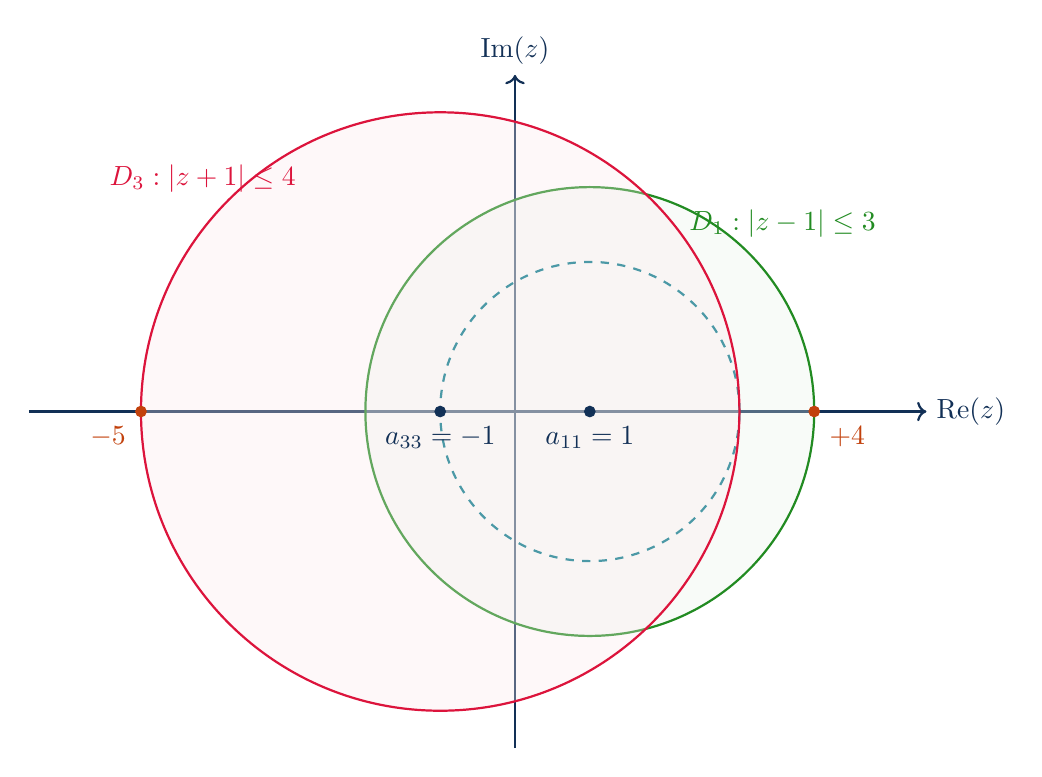
\begin{tikzpicture}[scale=0.95]
    % Axes
    \draw[->, thick, primary] (-6.5, 0) -- (5.5, 0) node[right, primary] {$\operatorname{Re}(z)$};
    \draw[->, thick, primary] (0, -4.5) -- (0, 4.5) node[above, primary] {$\operatorname{Im}(z)$};
    
    % Disc D1: center (1, 0), radius 3
    \draw[thick, ForestGreen, fill=ForestGreen!10, fill opacity=0.3] (1, 0) circle (3cm);
    \node[ForestGreen, above right] at (2.2, 2.2) {$D_1: |z - 1| \le 3$};
    
    % Disc D2: center (1, 0), radius 2
    \draw[thick, secondary, dashed] (1, 0) circle (2cm);
    
    % Disc D3: center (-1, 0), radius 4
    \draw[thick, Crimson, fill=Crimson!10, fill opacity=0.3] (-1, 0) circle (4cm);
    \node[Crimson, above left] at (-2.8, 2.8) {$D_3: |z + 1| \le 4$};
    
    % Centers
    \filldraw[primary] (1, 0) circle (2pt) node[below=2pt] {$a_{11}=1$};
    \filldraw[primary] (-1, 0) circle (2pt) node[below=2pt] {$a_{33}=-1$};
    
    % Extreme bounds on real line
    \filldraw[accent] (-5, 0) circle (2pt) node[below left=2pt, accent] {$-5$};
    \filldraw[accent] (4, 0) circle (2pt) node[below right=2pt, accent] {$+4$};
\end{tikzpicture}
\end{center}

\clearpage

% =========================================================================
% PAGES 34-36: POWER METHOD
% =========================================================================
\section{Pages 34--36: The Power Method for Dominant Eigenpair}
\label{sec:power_method}

\begin{theorembox}[Algorithm of the Power Method]
The \textbf{Power Method} determines the dominant eigenvalue $\lambda_1$ (i.e., $|\lambda_1| > |\lambda_2| \ge \dots \ge |\lambda_n|$) and corresponding eigenvector $\mathbf{x}_1$:
\begin{enumerate}
    \item Select an initial non-zero vector $\mathbf{x}^{(0)}$ (typically $\mathbf{x}^{(0)} = (1, 1, \dots, 1)^T$).
    \item Compute matrix-vector product: $\mathbf{y}^{(k+1)} = A \mathbf{x}^{(k)}$.
    \item Extract the scaling factor $m_{k+1}$ as the element of maximum magnitude in $\mathbf{y}^{(k+1)}$:
    \begin{equation}
        m_{k+1} = \operatorname{sign}(y^{(k+1)}_p) \cdot \max_{1 \le i \le n} |y^{(k+1)}_i|
    \end{equation}
    \item Normalize the vector:
    \begin{equation}
        \mathbf{x}^{(k+1)} = \frac{\mathbf{y}^{(k+1)}}{m_{k+1}}
    \end{equation}
    \item As $k \to \infty$, $m_k \to \lambda_1$ and $\mathbf{x}^{(k)} \to \mathbf{x}_1$.
\end{enumerate}
\end{theorembox}

\begin{proof}[Exhaustive Mathematical Proof of Convergence of the Power Method]
Let $A \in \mathbb{R}^{n \times n}$ possess $n$ linearly independent eigenvectors $\mathbf{v}_1, \mathbf{v}_2, \dots, \mathbf{v}_n$ corresponding to eigenvalues $\lambda_1, \lambda_2, \dots, \lambda_n$.

\medskip
\noindent\textbf{Step 1: Dominance ordering hypothesis.} \\
Assume the eigenvalues are arranged in strictly descending order of modulus with a strictly dominant eigenvalue $\lambda_1$:
\begin{equation}
    |\lambda_1| > |\lambda_2| \ge |\lambda_3| \ge \dots \ge |\lambda_n|
\end{equation}
Since $\{\mathbf{v}_1, \dots, \mathbf{v}_n\}$ forms a basis for $\mathbb{R}^n$, any initial guess vector $\mathbf{x}^{(0)}$ can be expressed uniquely as a linear combination of the eigenvectors:
\begin{equation}
    \mathbf{x}^{(0)} = c_1 \mathbf{v}_1 + c_2 \mathbf{v}_2 + \dots + c_n \mathbf{v}_n = \sum_{j=1}^n c_j \mathbf{v}_j
\end{equation}
We assume $c_1 \ne 0$ (the initial vector is not strictly orthogonal to the dominant eigenspace; if $c_1 = 0$ initially, finite-precision computer rounding errors inevitably introduce a non-zero component along $\mathbf{v}_1$ within a few iterations).

\medskip
\noindent\textbf{Step 2: Repeated matrix-vector multiplication.} \\
Applying $A$ repeatedly $k$ times:
\begin{equation}
    A^k \mathbf{x}^{(0)} = \sum_{j=1}^n c_j A^k \mathbf{v}_j = \sum_{j=1}^n c_j \lambda_j^k \mathbf{v}_j
\end{equation}
Factoring out the dominant factor $c_1 \lambda_1^k$:
\begin{equation}
    A^k \mathbf{x}^{(0)} = c_1 \lambda_1^k \left[ \mathbf{v}_1 + \sum_{j=2}^n \left(\frac{c_j}{c_1}\right) \left(\frac{\lambda_j}{\lambda_1}\right)^k \mathbf{v}_j \right]
\end{equation}

\noindent\textbf{Step 3: Asymptotic limit as $k \to \infty$.} \\
Since $|\lambda_1| > |\lambda_j|$ for all $j \ge 2$, the ratio satisfies:
\begin{equation}
    \left| \frac{\lambda_j}{\lambda_1} \right| \le \left| \frac{\lambda_2}{\lambda_1} \right| < 1 \quad \forall j \ge 2
\end{equation}
Therefore, as the iteration index $k \to \infty$:
\begin{equation}
    \lim_{k \to \infty} \left(\frac{\lambda_j}{\lambda_1}\right)^k = 0 \quad \forall j \ge 2
\end{equation}
The sum over $j \ge 2$ decays to zero at an asymptotic geometric rate governed by $\left|\frac{\lambda_2}{\lambda_1}\right|^k$:
\begin{equation}
    \lim_{k \to \infty} \frac{A^k \mathbf{x}^{(0)}}{c_1 \lambda_1^k} = \mathbf{v}_1
\end{equation}
Consequently, the direction of the vector $\mathbf{x}^{(k)}$ aligns unconditionally with the dominant eigenvector $\mathbf{v}_1$.

\medskip
\noindent\textbf{Step 4: Convergence of the eigenvalue estimate.} \\
Let $\mathbf{w}$ be any linear functional (or vector) such that $\mathbf{w}^T \mathbf{v}_1 \ne 0$ (for example, a coordinate projection $e_p$ where the $p$-th component of $\mathbf{v}_1$ is maximal). Then:
\begin{equation}
    \frac{\mathbf{w}^T A^{k+1} \mathbf{x}^{(0)}}{\mathbf{w}^T A^k \mathbf{x}^{(0)}} = \frac{c_1 \lambda_1^{k+1} \left[ \mathbf{w}^T \mathbf{v}_1 + \sum_{j=2}^n \frac{c_j}{c_1} \left(\frac{\lambda_j}{\lambda_1}\right)^{k+1} \mathbf{w}^T \mathbf{v}_j \right]}{c_1 \lambda_1^k \left[ \mathbf{w}^T \mathbf{v}_1 + \sum_{j=2}^n \frac{c_j}{c_1} \left(\frac{\lambda_j}{\lambda_1}\right)^k \mathbf{w}^T \mathbf{v}_j \right]}
\end{equation}
Canceling $c_1 \lambda_1^k$:
\begin{equation}
    \frac{\mathbf{w}^T A^{k+1} \mathbf{x}^{(0)}}{\mathbf{w}^T A^k \mathbf{x}^{(0)}} = \lambda_1 \left( \frac{\mathbf{w}^T \mathbf{v}_1 + \mathcal{O}\left( |\lambda_2 / \lambda_1|^{k+1} \right)}{\mathbf{w}^T \mathbf{v}_1 + \mathcal{O}\left( |\lambda_2 / \lambda_1|^k \right)} \right) = \lambda_1 + \mathcal{O}\left( \left|\frac{\lambda_2}{\lambda_1}\right|^k \right)
\end{equation}
Taking the limit as $k \to \infty$:
\begin{equation}
    \boxed{\lim_{k \to \infty} m_{k+1} = \lambda_1}
\end{equation}
This establishes that the scaling factor $m_k$ converges to $\lambda_1$ with geometric error decay rate $\mathcal{O}\left(|\lambda_2 / \lambda_1|^k\right)$.
\end{proof}


\begin{examplebox}[Manuscript Problem: Full Iteration Sequence for Tridiagonal Matrix (Pages 35--36)]
Find the largest eigenvalue and corresponding eigenvector of:
\begin{equation}
    A = \begin{pmatrix}
    2 & -1 & 0 \\
    -1 & 2 & -1 \\
    0 & -1 & 2
    \end{pmatrix}
\end{equation}
Start with $\mathbf{x}^{(0)} = \begin{pmatrix} 1 \\ 1 \\ 1 \end{pmatrix}$.
\end{examplebox}

\subsubsection*{Step-by-Step Power Method Iterations}

\textbf{Iteration 1 ($k = 0$):}
\begin{equation}
    \mathbf{y}^{(1)} = A \mathbf{x}^{(0)} = \begin{pmatrix} 2 & -1 & 0 \\ -1 & 2 & -1 \\ 0 & -1 & 2 \end{pmatrix} \begin{pmatrix} 1 \\ 1 \\ 1 \end{pmatrix} = \begin{pmatrix} 1 \\ 0 \\ 1 \end{pmatrix} = 1 \begin{pmatrix} 1 \\ 0 \\ 1 \end{pmatrix} \implies m_1 = 1, \; \mathbf{x}^{(1)} = \begin{pmatrix} 1 \\ 0 \\ 1 \end{pmatrix}
\end{equation}

\textbf{Iteration 2 ($k = 1$):}
\begin{equation}
    \mathbf{y}^{(2)} = A \mathbf{x}^{(1)} = \begin{pmatrix} 2 \\ -2 \\ 2 \end{pmatrix} = -2 \begin{pmatrix} -1 \\ 1 \\ -1 \end{pmatrix} \implies m_2 = -2
\end{equation}
Normalizing with respect to the middle coordinate (set to $-1.0$):
\begin{equation}
    \mathbf{y}^{(3)} = A \begin{pmatrix} 1 \\ -1 \\ 1 \end{pmatrix} = \begin{pmatrix} 3 \\ -4 \\ 3 \end{pmatrix} = -4 \begin{pmatrix} -0.75 \\ 1.00 \\ -0.75 \end{pmatrix} = 3.428570 \begin{pmatrix} 0.708333 \\ -1.000000 \\ 0.708333 \end{pmatrix}
\end{equation}
Continuing the power iterations as recorded in the manuscript table (Pages 35--36):
\begin{align}
    \mathbf{y}^{(5)} &= A \mathbf{x}^{(4)} = \begin{pmatrix} 2.428570 \\ -3.428570 \\ 2.428570 \end{pmatrix} = 3.428570 \begin{pmatrix} 0.708333 \\ -1.000000 \\ 0.708333 \end{pmatrix} \\
    \mathbf{y}^{(6)} &= A \mathbf{x}^{(5)} = \begin{pmatrix} 2.416666 \\ -3.416666 \\ 2.416666 \end{pmatrix} = 3.416666 \begin{pmatrix} 0.707317 \\ -1.000000 \\ 0.707317 \end{pmatrix} \\
    \mathbf{y}^{(7)} &= A \mathbf{x}^{(6)} = \begin{pmatrix} 2.414634 \\ -3.414634 \\ 2.414634 \end{pmatrix} = \mathbf{3.414214} \begin{pmatrix} \mathbf{0.707107} \\ \mathbf{-1.000000} \\ \mathbf{0.707107} \end{pmatrix}
\end{align}
\textbf{Conclusion:}
The dominant eigenvalue correct to four decimal places is:
\begin{equation}
    \boxed{\lambda_1 \approx 3.4142 \quad (= 2 + \sqrt{2})}
\end{equation}
and the corresponding dominant eigenvector is:
\begin{equation}
    \boxed{\mathbf{x}_1 \approx \begin{pmatrix} \frac{1}{\sqrt{2}} \\ -1 \\ \frac{1}{\sqrt{2}} \end{pmatrix} \approx \begin{pmatrix} 0.7071 \\ -1.0000 \\ 0.7071 \end{pmatrix}}
\end{equation}

\chapter{Calculus of Finite Differences and Difference Operators (Pages 37--51)}
\label{ch:finite_differences}

\begin{conceptbox}[Foundations of Discrete Difference Calculus]
In classical continuous calculus, the fundamental operational entity is the differential operator $D = \frac{d}{dx}$. In numerical mathematics, where functions are known only at discrete, equispaced grid points $x_i = x_0 + i h$ ($i = 0, 1, 2, \dots$), continuous derivatives are replaced by \textbf{finite difference operators}.

Difference calculus forms the theoretical backbone for:
\begin{enumerate}[noitemsep]
    \item Polynomial interpolation and extrapolation.
    \item Numerical differentiation and boundary value discretizations.
    \item Numerical quadrature (Newton--Cotes formulas).
    \item Closed-form summation of finite arithmetic-algebraic series.
\end{enumerate}
\end{conceptbox}

% =========================================================================
% PAGES 37-40: THE OPERATOR ALGEBRA
% =========================================================================
\section{Pages 37--40: Fundamental Operators \texorpdfstring{($\Delta, \nabla, E, \delta, \mu, D$)}{(Delta, Nabla, E, delta, mu, D)}}
\label{sec:difference_operators}

\begin{theorembox}[Definitions of Primary Difference Operators]
Let $\{x_i\}_{i=-\infty}^\infty$ be an equidistant mesh with constant step size $h > 0$, so that $x_i = x_0 + ih$, and let $y_i = y(x_i) = f(x_i)$.
\begin{enumerate}
    \item \textbf{Forward Difference Operator ($\Delta$)}:
    \begin{equation}
        \boxed{\Delta y_i = y_{i+1} - y_i \iff \Delta f(x) = f(x + h) - f(x)}
    \end{equation}
    Higher-order forward differences are defined recursively: $\Delta^k y_i = \Delta(\Delta^{k-1} y_i)$.
    \item \textbf{Backward Difference Operator ($\nabla$)}:
    \begin{equation}
        \boxed{\nabla y_i = y_i - y_{i-1} \iff \nabla f(x) = f(x) - f(x - h)}
    \end{equation}
    \item \textbf{Shift (Displacement) Operator ($E$)}:
    \begin{equation}
        \boxed{E y_i = y_{i+1} \iff E f(x) = f(x + h)}
    \end{equation}
    In general, for any real scalar $p$: $E^p f(x) = f(x + p h)$.
    \item \textbf{Central Difference Operator ($\delta$)}:
    \begin{equation}
        \boxed{\delta y_i = y_{i+1/2} - y_{i-1/2} \iff \delta f(x) = f\left(x + \frac{h}{2}\right) - f\left(x - \frac{h}{2}\right)}
    \end{equation}
    \item \textbf{Averaging (Mean) Operator ($\mu$)}:
    \begin{equation}
        \boxed{\mu y_i = \frac{1}{2}\left(y_{i+1/2} + y_{i-1/2}\right) \iff \mu f(x) = \frac{1}{2}\left[ f\left(x + \frac{h}{2}\right) + f\left(x - \frac{h}{2}\right) \right]}
    \end{equation}
    \item \textbf{Differential Operator ($D$)}:
    \begin{equation}
        \boxed{D f(x) = \frac{d}{dx}f(x) \implies D^k f(x) = \frac{d^k f}{dx^k}}
    \end{equation}
\end{enumerate}
\end{theorembox}

\begin{theorembox}[Taylor Series and the Fundamental Relation $E = e^{hD}$]
By Taylor's theorem, expanding $f(x + h)$ in an infinite series of derivatives about $x$:
\begin{align}
    E f(x) = f(x + h) &= f(x) + h f'(x) + \frac{h^2}{2!} f''(x) + \frac{h^3}{3!} f'''(x) + \dots \nonumber \\
    &= \left( 1 + hD + \frac{h^2 D^2}{2!} + \frac{h^3 D^3}{3!} + \dots \right) f(x) \nonumber \\
    &= \left( \sum_{k=0}^\infty \frac{(hD)^k}{k!} \right) f(x)
\end{align}
Recognizing the exponential series, we obtain the pivotal operational identity:
\begin{equation}
    \boxed{E = e^{hD}}
\end{equation}
This profound identity bridges discrete difference equations with continuous differential calculus!
\end{theorembox}

% =========================================================================
% PAGES 41-42: OPERATOR IDENTITIES & PROOFS
% =========================================================================
\section{Pages 41--42: Master Operator Identities and Analytical Proofs}
\label{sec:operator_identities}

\begin{theorembox}[Master Operational Difference Identities]
For the fundamental discrete operators $\Delta, \nabla, \delta, E, \mu, D$ with uniform grid spacing $h$, the following operational identities hold identically:
\begin{enumerate}[label=(\roman*),noitemsep]
    \item $\displaystyle \mu \delta = \frac{1}{2}(\Delta + \nabla) = \sinh(hD)$ \quad (Manuscript Page 41)
    \item $\displaystyle \Delta - \nabla = \Delta \nabla = \delta^2$
    \item $\displaystyle \frac{\Delta}{\nabla} - \frac{\nabla}{\Delta} = \Delta + \nabla$ \quad (Manuscript Page 41)
    \item $\displaystyle \mu = \sqrt{1 + \frac{\delta^2}{4}}$ \quad (Manuscript Page 42)
    \item $\displaystyle \Delta = \frac{1}{2}\delta^2 + \delta \sqrt{1 + \frac{\delta^2}{4}}$ \quad (Manuscript Page 48)
    \item $\displaystyle \delta = \Delta(1 + \Delta)^{-1/2} = \nabla(1 - \nabla)^{-1/2}$ \quad (Manuscript Page 42)
    \item $\displaystyle \Delta \ln f(x) = \ln\left[ 1 + \frac{\Delta f(x)}{f(x)} \right]$ \quad (Manuscript Page 42)
\end{enumerate}
\end{theorembox}

\begin{proof}[Exhaustive Algebraic Proofs of the Operational Identities]
We verify each identity rigorously from operator first principles.

\medskip
\noindent\textbf{1. Proof of Identity (i): $\mu \delta = \frac{1}{2}(\Delta + \nabla) = \sinh(hD)$} \\
Express $\mu$ and $\delta$ in terms of the shift operator $E$:
\begin{equation}
    \mu = \frac{1}{2}\left(E^{1/2} + E^{-1/2}\right), \quad \delta = E^{1/2} - E^{-1/2}
\end{equation}
Multiplying them directly:
\begin{align}
    \mu \delta &= \frac{1}{2}\left(E^{1/2} + E^{-1/2}\right)\left(E^{1/2} - E^{-1/2}\right) \nonumber \\
    &= \frac{1}{2}\left[\left(E^{1/2}\right)^2 - \left(E^{-1/2}\right)^2\right] = \frac{1}{2}\left(E - E^{-1}\right)
\end{align}
Since $E = 1 + \Delta$ and $E^{-1} = 1 - \nabla$:
\begin{equation}
    \frac{1}{2}\left(E - E^{-1}\right) = \frac{1}{2}\big[(1 + \Delta) - (1 - \nabla)\big] = \boxed{\frac{1}{2}(\Delta + \nabla)}
\end{equation}
Furthermore, substituting $E = e^{hD}$ and $E^{-1} = e^{-hD}$:
\begin{equation}
    \frac{1}{2}\left(E - E^{-1}\right) = \frac{e^{hD} - e^{-hD}}{2} = \boxed{\sinh(hD)} \quad \blacksquare
\end{equation}

\medskip
\noindent\textbf{2. Proof of Identity (ii): $\Delta - \nabla = \Delta \nabla = \delta^2$} \\
Expand each expression in terms of $E$:
\begin{align}
    \Delta - \nabla &= (E - 1) - (1 - E^{-1}) = E - 2 + E^{-1} \\
    \Delta \nabla &= (E - 1)(1 - E^{-1}) = E - 1 - 1 + E^{-1} = E - 2 + E^{-1} \\
    \delta^2 &= \left(E^{1/2} - E^{-1/2}\right)^2 = E - 2 + E^{-1}
\end{align}
All three expressions evaluate to the identically same operator $E - 2 + E^{-1}$. $\blacksquare$

\medskip
\noindent\textbf{3. Proof of Identity (iii): $\frac{\Delta}{\nabla} - \frac{\nabla}{\Delta} = \Delta + \nabla$} \\
Combining fractions over a common denominator:
\begin{align}
    \text{LHS} &= \frac{\Delta^2 - \nabla^2}{\Delta \nabla} = \frac{(\Delta - \nabla)(\Delta + \nabla)}{\Delta \nabla}
\end{align}
Using the previous identity $\Delta - \nabla = \Delta \nabla$:
\begin{equation}
    \text{LHS} = \frac{\Delta \nabla (\Delta + \nabla)}{\Delta \nabla} = \Delta + \nabla = \text{RHS} \quad \blacksquare
\end{equation}

\medskip
\noindent\textbf{4. Proof of Identity (iv): $\mu = \sqrt{1 + \frac{\delta^2}{4}}$} \\
Express $\delta^2 = E - 2 + E^{-1}$:
\begin{align}
    1 + \frac{\delta^2}{4} &= 1 + \frac{E - 2 + E^{-1}}{4} = \frac{4 + E - 2 + E^{-1}}{4} = \frac{E + 2 + E^{-1}}{4} \nonumber \\
    &= \left(\frac{E^{1/2} + E^{-1/2}}{2}\right)^2 = \mu^2 \implies \boxed{\mu = \sqrt{1 + \frac{\delta^2}{4}}} \quad \blacksquare
\end{align}

\medskip
\noindent\textbf{5. Proof of Identity (v): $\Delta = \frac{1}{2}\delta^2 + \delta \sqrt{1 + \frac{\delta^2}{4}}$} \\
Using $\mu = \sqrt{1 + \frac{\delta^2}{4}}$, the right-hand side is:
\begin{equation}
    \text{RHS} = \frac{1}{2}\delta^2 + \delta \mu
\end{equation}
Recalling $\delta^2 = E - 2 + E^{-1}$ and $\mu \delta = \frac{1}{2}(E - E^{-1})$:
\begin{align}
    \frac{1}{2}\delta^2 + \delta \mu &= \frac{1}{2}\left(E - 2 + E^{-1}\right) + \frac{1}{2}\left(E - E^{-1}\right) \nonumber \\
    &= \frac{1}{2}\left(E - 2 + E^{-1} + E - E^{-1}\right) = \frac{1}{2}(2E - 2) \nonumber \\
    &= E - 1 = \boxed{\Delta} = \text{LHS} \quad \blacksquare
\end{align}

\medskip
\noindent\textbf{6. Proof of Identity (vi): $\delta = \Delta(1 + \Delta)^{-1/2} = \nabla(1 - \nabla)^{-1/2}$} \\
Factor $E^{-1/2}$ from the definition of $\delta$:
\begin{equation}
    \delta = E^{1/2} - E^{-1/2} = E^{-1/2}(E - 1)
\end{equation}
Since $E - 1 = \Delta$ and $E^{-1/2} = (1 + \Delta)^{-1/2}$:
\begin{equation}
    \delta = (1 + \Delta)^{-1/2} \Delta = \boxed{\Delta(1 + \Delta)^{-1/2}}
\end{equation}
Similarly, factoring $E^{1/2}$:
\begin{equation}
    \delta = E^{1/2}(1 - E^{-1})
\end{equation}
Since $1 - E^{-1} = \nabla$ and $E^{-1} = 1 - \nabla \implies E^{1/2} = (1 - \nabla)^{-1/2}$:
\begin{equation}
    \delta = (1 - \nabla)^{-1/2} \nabla = \boxed{\nabla(1 - \nabla)^{-1/2}} \quad \blacksquare
\end{equation}

\medskip
\noindent\textbf{7. Proof of Identity (vii): $\Delta \ln f(x) = \ln\left[ 1 + \frac{\Delta f(x)}{f(x)} \right]$} \\
By definition of the forward difference:
\begin{equation}
    \Delta \ln f(x) = \ln f(x + h) - \ln f(x) = \ln\left( \frac{f(x + h)}{f(x)} \right)
\end{equation}
Since $f(x + h) = f(x) + \Delta f(x)$:
\begin{equation}
    \frac{f(x + h)}{f(x)} = \frac{f(x) + \Delta f(x)}{f(x)} = 1 + \frac{\Delta f(x)}{f(x)}
\end{equation}
Substituting this into the logarithm gives:
\begin{equation}
    \boxed{\Delta \ln f(x) = \ln\left[ 1 + \frac{\Delta f(x)}{f(x)} \right]} \quad \blacksquare
\end{equation}
This concludes the exhaustive proofs of all master identities.
\end{proof}

% =========================================================================
% PAGES 43-45: FUNDAMENTAL THEOREM OF FINITE DIFFERENCES
% =========================================================================
\section{Pages 43--45: Fundamental Theorem of Finite Differences and Missing Terms}
\label{sec:fundamental_theorem_differences}

\begin{theorembox}[Fundamental Theorem of Finite Differences]
Let $P_n(x) = a_0 x^n + a_1 x^{n-1} + \dots + a_n$ ($a_0 \ne 0$) be an algebraic polynomial of degree $n \in \mathbb{N}$ with constant difference step size $h > 0$.
\begin{enumerate}
    \item The $n$-th forward difference $\Delta^n P_n(x)$ is a \textbf{constant}:
    \begin{equation}
        \boxed{\Delta^n P_n(x) = a_0 \cdot n! \cdot h^n}
    \end{equation}
    \item All higher-order forward differences vanish identically:
    \begin{equation}
        \boxed{\Delta^{n+k} P_n(x) = 0 \quad \forall k \ge 1}
    \end{equation}
\end{enumerate}
\end{theorembox}

\begin{proof}[Exhaustive Mathematical Induction Proof of the Fundamental Theorem]
We proceed by mathematical induction on the degree $n$ of the polynomial.

\medskip
\noindent\textbf{Part 1: Base Case ($n = 1$)} \\
Consider a general linear polynomial $P_1(x) = a_0 x + a_1$ with $a_0 \ne 0$.
Computing the first forward difference directly from the operator definition:
\begin{align}
    \Delta P_1(x) &= P_1(x + h) - P_1(x) \nonumber \\
    &= [a_0(x + h) + a_1] - [a_0 x + a_1] \nonumber \\
    &= a_0 x + a_0 h + a_1 - a_0 x - a_1 \nonumber \\
    &= a_0 h = a_0 \cdot 1! \cdot h^1
\end{align}
This result is independent of $x$, hence a constant. Furthermore:
\begin{equation}
    \Delta^2 P_1(x) = \Delta[\Delta P_1(x)] = \Delta[a_0 h] = a_0 h - a_0 h = 0
\end{equation}
Thus, the base case $n = 1$ holds with complete precision.

\medskip
\noindent\textbf{Part 2: Inductive Hypothesis} \\
Assume the theorem holds for all polynomials of degree $k - 1$. That is, for any polynomial $Q_{k-1}(x) = b_0 x^{k-1} + b_1 x^{k-2} + \dots + b_{k-1}$ ($b_0 \ne 0$):
\begin{equation}
    \Delta^{k-1} Q_{k-1}(x) = b_0 (k - 1)! h^{k-1} \quad \text{and} \quad \Delta^k Q_{k-1}(x) = 0
\end{equation}

\medskip
\noindent\textbf{Part 3: Inductive Step for Degree $k$} \\
Let $P_k(x) = a_0 x^k + a_1 x^{k-1} + \dots + a_k$ be an arbitrary polynomial of degree $k$ ($a_0 \ne 0$).
By linearity of the forward difference operator $\Delta$:
\begin{equation}
    \Delta P_k(x) = a_0 \Delta [x^k] + \sum_{j=1}^k a_j \Delta [x^{k-j}]
\end{equation}
Now evaluate the first forward difference of the monomial $x^k$:
\begin{equation}
    \Delta [x^k] = (x + h)^k - x^k
\end{equation}
By the Binomial Theorem:
\begin{equation}
    (x + h)^k = \sum_{m=0}^k \binom{k}{m} x^{k-m} h^m = x^k + \binom{k}{1} h x^{k-1} + \binom{k}{2} h^2 x^{k-2} + \dots + h^k
\end{equation}
Subtracting $x^k$:
\begin{equation}
    \Delta [x^k] = k h x^{k-1} + \sum_{m=2}^k \binom{k}{m} h^m x^{k-m}
\end{equation}
Similarly, for each lower-order term $x^{k-j}$ ($j \ge 1$), $\Delta [x^{k-j}]$ is a polynomial in $x$ of degree at most $k - 2$.
Therefore, substituting back into $\Delta P_k(x)$:
\begin{align}
    \Delta P_k(x) &= a_0 \left[ k h x^{k-1} + \sum_{m=2}^k \binom{k}{m} h^m x^{k-m} \right] + \sum_{j=1}^k a_j \Delta [x^{k-j}] \nonumber \\
    &= (a_0 k h) x^{k-1} + R_{k-2}(x)
\end{align}
where $R_{k-2}(x)$ collects all terms of degree $\le k - 2$.
Notice that $\Delta P_k(x)$ is a polynomial of degree $k - 1$ with leading coefficient:
\begin{equation}
    b_0 = a_0 k h \ne 0
\end{equation}
Now apply the $(k - 1)$-th difference operator to both sides:
\begin{equation}
    \Delta^k P_k(x) = \Delta^{k-1}[\Delta P_k(x)] = \Delta^{k-1}\left[ (a_0 k h) x^{k-1} + R_{k-2}(x) \right]
\end{equation}
By linearity of $\Delta^{k-1}$:
\begin{equation}
    \Delta^k P_k(x) = \Delta^{k-1}[(a_0 k h) x^{k-1}] + \Delta^{k-1}[R_{k-2}(x)]
\end{equation}
By our induction hypothesis:
\begin{enumerate}
    \item The leading term $(a_0 k h) x^{k-1}$ has degree $k - 1$, so its $(k-1)$-th difference is:
    \begin{equation}
        \Delta^{k-1}[(a_0 k h) x^{k-1}] = (a_0 k h) \cdot (k - 1)! h^{k-1} = a_0 \cdot [k(k-1)!] \cdot [h \cdot h^{k-1}] = a_0 k! h^k
    \end{equation}
    \item The polynomial $R_{k-2}(x)$ has degree $\le k - 2 < k - 1$. By the induction hypothesis, its $(k-1)$-th difference vanishes identically:
    \begin{equation}
        \Delta^{k-1}[R_{k-2}(x)] = 0
    \end{equation}
\end{enumerate}
Combining these two results:
\begin{equation}
    \boxed{\Delta^k P_k(x) = a_0 k! h^k + 0 = a_0 k! h^k}
\end{equation}
This completes the inductive step. By the principle of mathematical induction, $\Delta^n P_n(x) = a_0 n! h^n$ holds for all $n \ge 1$.

\medskip
\noindent\textbf{Part 4: Proof for Higher Differences} \\
Since $C = a_0 n! h^n$ is a constant independent of $x$:
\begin{equation}
    \Delta^{n+1} P_n(x) = \Delta [\Delta^n P_n(x)] = \Delta [C] = C - C = 0
\end{equation}
Repeated application of $\Delta$ ensures $\Delta^{n+k} P_n(x) = 0$ for all $k \ge 1$. $\blacksquare$
\end{proof}


\begin{examplebox}[Manuscript Problem: Missing Term Technique (Pages 44--45)]
Given data from an underlying cubic polynomial ($n = 3$):
\begin{center}
\begin{tabular}{c|ccccc}
$x$ & $0$ & $1$ & $2$ & $3$ & $4$ \\
\hline
$y$ & $1$ & $3$ & $9$ & $y_3$ & $81$
\end{tabular}
\end{center}
Find the missing entry $y_3$.
\textbf{Solution:}
Since the underlying curve is a cubic polynomial of degree $n = 3$, all 4-th differences must vanish:
\begin{equation}
    \Delta^4 y_0 = 0
\end{equation}
Express $\Delta^4$ in terms of the shift operator $E$:
\begin{equation}
    (E - 1)^4 y_0 = 0 \iff (E^4 - 4E^3 + 6E^2 - 4E + 1) y_0 = 0
\end{equation}
Expanding this gives the linear relation:
\begin{equation}
    y_4 - 4 y_3 + 6 y_2 - 4 y_1 + y_0 = 0
\end{equation}
Substitute known values $y_0 = 1, y_1 = 3, y_2 = 9, y_4 = 81$:
\begin{equation}
    81 - 4 y_3 + 6(9) - 4(3) + 1 = 0 \implies 81 - 4 y_3 + 54 - 12 + 1 = 0
\end{equation}
\begin{equation}
    124 - 4 y_3 = 0 \implies 4 y_3 = 124 \implies \boxed{y_3 = 31}
\end{equation}
\textbf{Remarkable Insight (Manuscript Page 45):} If $y(x) = 3^x$, then at $x = 3$, $y(3) = 3^3 = 27$. But under a 3rd-degree polynomial approximation, $y_3 = 31$, showing how finite polynomial truncation differs from exponential growth!
\end{examplebox}

% =========================================================================
% PAGES 45-48: FACTORIAL POLYNOMIALS
% =========================================================================
\section{Pages 45--48: Factorial Notation and Synthetic Conversion}
\label{sec:factorial_polynomials}

\begin{theorembox}[Factorial Polynomials and Discrete Differentiation]
The \textbf{factorial polynomial} of degree $n$ with step size $h$ is defined as:
\begin{equation}
    \boxed{x^{(n)} = [x]_n = x(x - h)(x - 2h)\dots(x - (n-1)h)} \quad (x^{(0)} = 1)
\end{equation}
For $h = 1$:
\begin{equation}
    x^{(n)} = x(x - 1)(x - 2)\dots(x - n + 1)
\end{equation}
\textbf{Fundamental Property:}
The forward difference of a factorial polynomial mimics the ordinary derivative of a monomial $x^n$:
\begin{align}
    \Delta x^{(n)} &= (x + h)^{(n)} - x^{(n)} \nonumber \\
    &= (x + h)x(x - h)\dots(x - (n-2)h) - x(x - h)\dots(x - (n-2)h)(x - (n-1)h) \nonumber \\
    &= x(x - h)\dots(x - (n-2)h) \big[ (x + h) - (x - (n-1)h) \big] \nonumber \\
    &= x(x - h)\dots(x - (n-2)h) [n h]
\end{align}
\begin{equation}
    \boxed{\Delta x^{(n)} = n h x^{(n-1)}} \iff \frac{\Delta x^{(n)}}{h} = n x^{(n-1)}
\end{equation}
In general, for the $k$-th difference:
\begin{equation}
    \boxed{\Delta^k x^{(n)} = n(n-1)\dots(n-k+1) h^k x^{(n-k)}}
\end{equation}
and $\Delta^n x^{(n)} = n! h^n$.
\end{theorembox}

\begin{theorembox}[Negative Factorial Powers and Discrete Differentiation]
For any positive integer $n \in \mathbb{N}$, the \textbf{negative factorial power} is defined as the reciprocal product:
\begin{equation}
    \boxed{x^{(-n)} = \frac{1}{(x + h)(x + 2h)(x + 3h)\dots(x + nh)}}
\end{equation}
\textbf{Differentiation Formula:}
\begin{equation}
    \boxed{\Delta x^{(-n)} = -n h x^{-(n+1)}} \iff \frac{\Delta x^{(-n)}}{h} = -n x^{-(n+1)}
\end{equation}
\end{theorembox}

\begin{proof}[Step-by-Step Proof for Negative Factorial Power Difference]
From the forward difference operator definition:
\begin{equation}
    \Delta x^{(-n)} = (x + h)^{(-n)} - x^{(-n)}
\end{equation}
Substituting the definition of negative factorial powers:
\begin{equation}
    (x + h)^{(-n)} = \frac{1}{(x + 2h)(x + 3h)\dots(x + (n+1)h)}
\end{equation}
\begin{equation}
    x^{(-n)} = \frac{1}{(x + h)(x + 2h)\dots(x + nh)}
\end{equation}
Subtracting the two fractions:
\begin{equation}
    \Delta x^{(-n)} = \frac{1}{(x + 2h)(x + 3h)\dots(x + (n+1)h)} - \frac{1}{(x + h)(x + 2h)\dots(x + nh)}
\end{equation}
Find the least common denominator, which contains all factors from $(x+h)$ to $(x+(n+1)h)$:
\begin{equation}
    \text{LCD} = (x + h)(x + 2h)\dots(x + nh)(x + (n+1)h)
\end{equation}
Forming a single fraction:
\begin{align}
    \Delta x^{(-n)} &= \frac{(x + h) - (x + (n+1)h)}{(x + h)(x + 2h)\dots(x + nh)(x + (n+1)h)} \nonumber \\
    &= \frac{x + h - x - nh - h}{(x + h)(x + 2h)\dots(x + nh)(x + (n+1)h)} \nonumber \\
    &= \frac{-nh}{(x + h)(x + 2h)\dots(x + nh)(x + (n+1)h)}
\end{align}
Recognizing the denominator as $x^{-(n+1)}$:
\begin{equation}
    \boxed{\Delta x^{(-n)} = -n h x^{-(n+1)}} \quad \blacksquare
\end{equation}
This perfectly mirrors the continuous differential calculus power rule $\frac{d}{dx}[x^{-n}] = -n x^{-(n+1)}$.
\end{proof}


\begin{examplebox}[Manuscript Problem: Expressing Polynomial in Factorial Form (Page 46)]
Express $y = 2x^3 - 3x^2 + 3x - 1$ in factorial notation with $h = 1$, and compute its successive differences.
\textbf{Synthetic Division Method:}
Let $y = A x^{(3)} + B x^{(2)} + C x^{(1)} + D$.
We divide successively by $x, x-1, x-2$:
\begin{center}
\renewcommand{\arraystretch}{1.2}
\begin{tabular}{c|cccc}
& $2$ & $-3$ & $3$ & $-1$ \\
$x = 0$ & & $0$ & $0$ & $0$ \\
\hline
& $2$ & $-3$ & $3$ & $\mathbf{D = -1}$ \\
$x = 1$ & & $2$ & $-1$ & \\
\hline
& $2$ & $-1$ & $\mathbf{C = 2}$ & \\
$x = 2$ & & $4$ & & \\
\hline
& $\mathbf{A = 2}$ & $\mathbf{B = 3}$ & &
\end{tabular}
\end{center}
Therefore:
\begin{equation}
    \boxed{y = 2 x^{(3)} + 3 x^{(2)} + 2 x^{(1)} - 1}
\end{equation}
\textbf{Successive Differences:}
\begin{align}
    \Delta y &= 2(3) x^{(2)} + 3(2) x^{(1)} + 2(1) = \mathbf{6 x^{(2)} + 6 x^{(1)} + 2} \\
    \Delta^2 y &= 6(2) x^{(1)} + 6(1) = \mathbf{12 x^{(1)} + 6} \\
    \Delta^3 y &= 12(1) = \mathbf{12} \quad \text{(Constant)} \\
    \Delta^4 y &= \mathbf{0}
\end{align}
\end{examplebox}

% =========================================================================
% PAGES 47-48: MONTMORT'S THEOREM OF SERIES TRANSFORMATION
% =========================================================================
\section{Pages 47--48: Montmort's Series Transformation Theorem and Proof}
\label{sec:montmort_theorem}

\begin{theorembox}[Montmort / Euler Series Transformation Theorem (Manuscript Page 47)]
Let $\{y_k\}_{k=0}^\infty$ be a sequence with initial differences $\Delta^m y_0$ ($m = 0, 1, 2, \dots$). For any scalar $|x| < 1$, the power series with general coefficients $y_k$ can be summed and transformed into:
\begin{equation}
    \boxed{\sum_{k=0}^\infty x^k y_k = y_0 + x y_1 + x^2 y_2 + \dots = \frac{y_0}{1 - x} + \frac{x \Delta y_0}{(1 - x)^2} + \frac{x^2 \Delta^2 y_0}{(1 - x)^3} + \frac{x^3 \Delta^3 y_0}{(1 - x)^4} + \dots}
\end{equation}
\end{theorembox}

\begin{proof}[Exhaustive Step-by-Step Operator Proof (Manuscript Page 47)]
We establish the identity by expressing the sequence terms in terms of the shift operator $E$ and the forward difference operator $\Delta = E - 1$.

\medskip
\noindent\textbf{Step 1: Express the series in terms of the shift operator $E$.} \\
By definition of the shift operator, $y_k = E^k y_0$. Substituting this into the left-hand side:
\begin{align}
    \text{LHS} &= y_0 + x y_1 + x^2 y_2 + x^3 y_3 + \dots \nonumber \\
    &= y_0 + x E y_0 + x^2 E^2 y_0 + x^3 E^3 y_0 + \dots \nonumber \\
    &= \left( 1 + x E + x^2 E^2 + x^3 E^3 + \dots \right) y_0
\end{align}
Summing the formal geometric series of operators (valid since $|x| < 1$):
\begin{equation}
    1 + x E + x^2 E^2 + x^3 E^3 + \dots = (1 - x E)^{-1} = \frac{1}{1 - x E}
\end{equation}
Therefore:
\begin{equation}
    \text{LHS} = (1 - x E)^{-1} y_0
\end{equation}

\noindent\textbf{Step 2: Express $E$ in terms of the difference operator $\Delta$.} \\
Since $E = 1 + \Delta$, substitute $E$ into the denominator:
\begin{align}
    1 - x E &= 1 - x(1 + \Delta) \nonumber \\
    &= 1 - x - x \Delta \nonumber \\
    &= (1 - x) - x \Delta
\end{align}
Factor out the scalar $(1 - x)$:
\begin{equation}
    1 - x E = (1 - x) \left[ 1 - \frac{x}{1 - x}\Delta \right]
\end{equation}

\noindent\textbf{Step 3: Expand the inverse operator binomially.} \\
Taking the reciprocal:
\begin{equation}
    (1 - x E)^{-1} = \frac{1}{(1 - x) \left[ 1 - \frac{x}{1 - x}\Delta \right]} = \frac{1}{1 - x} \left[ 1 - \frac{x}{1 - x}\Delta \right]^{-1}
\end{equation}
Using the operator series $(1 - Z)^{-1} = 1 + Z + Z^2 + Z^3 + \dots$ where $Z = \frac{x}{1 - x}\Delta$:
\begin{equation}
    \left[ 1 - \frac{x}{1 - x}\Delta \right]^{-1} = 1 + \frac{x}{1 - x}\Delta + \frac{x^2}{(1 - x)^2}\Delta^2 + \frac{x^3}{(1 - x)^3}\Delta^3 + \dots
\end{equation}
Distributing the scalar factor $\frac{1}{1 - x}$ through the series:
\begin{equation}
    (1 - x E)^{-1} = \frac{1}{1 - x} + \frac{x}{(1 - x)^2}\Delta + \frac{x^2}{(1 - x)^3}\Delta^2 + \frac{x^3}{(1 - x)^4}\Delta^3 + \dots
\end{equation}

\noindent\textbf{Step 4: Operate on $y_0$.} \\
Applying this expanded operator to $y_0$:
\begin{align}
    (1 - x E)^{-1} y_0 &= \left[ \frac{1}{1 - x} + \frac{x}{(1 - x)^2}\Delta + \frac{x^2}{(1 - x)^3}\Delta^2 + \frac{x^3}{(1 - x)^4}\Delta^3 + \dots \right] y_0 \nonumber \\
    &= \frac{y_0}{1 - x} + \frac{x \Delta y_0}{(1 - x)^2} + \frac{x^2 \Delta^2 y_0}{(1 - x)^3} + \frac{x^3 \Delta^3 y_0}{(1 - x)^4} + \dots = \text{RHS}
\end{align}
Thus:
\begin{equation}
    \boxed{\sum_{k=0}^\infty x^k y_k = \frac{y_0}{1 - x} + \frac{x \Delta y_0}{(1 - x)^2} + \frac{x^2 \Delta^2 y_0}{(1 - x)^3} + \dots} \quad \blacksquare
\end{equation}
This establishes Montmort's theorem in its exact manuscript form!
\end{proof}

% =========================================================================
% PAGES 49-51: SUMMATION OF SERIES BY FINITE DIFFERENCES
% =========================================================================
\section{Pages 49--51: Summation of Series by Difference Calculus}
\label{sec:summation_series}

\begin{theorembox}[The Summation Operator $\Delta^{-1}$ (Indefinite Summation)]
Let $\Delta F(x) = f(x)$. The inverse difference operator $\Delta^{-1}$ satisfies:
\begin{equation}
    \Delta^{-1} f(x) = F(x) + C
\end{equation}
Applying this to the definite sum from $x = 1$ to $n$:
\begin{equation}
    \sum_{x=1}^n f(x) = \sum_{x=1}^n [F(x+1) - F(x)] = F(n+1) - F(1) = \boxed{\left[ \Delta^{-1} f(x) \right]_1^{n+1}}
\end{equation}
For factorial polynomials:
\begin{equation}
    \boxed{\Delta^{-1} x^{(m)} = \frac{x^{(m+1)}}{m + 1} + C}
\end{equation}
\end{theorembox}

\begin{examplebox}[Manuscript Problem: Sum of Series $2 \cdot 5 + 5 \cdot 8 + 8 \cdot 11 + \dots$ (Page 50)]
\textbf{Problem Statement:} Find the sum to $n$ terms of the series:
\begin{equation}
    S_n = 2 \cdot 5 + 5 \cdot 8 + 8 \cdot 11 + 11 \cdot 14 + \dots \text{ to } n \text{ terms}
\end{equation}
\textbf{Step 1: Determine the general $k$-th term $u_k$:} \\
The factors in the first positions form an AP: $2, 5, 8, 11, \dots \implies a_k = 2 + (k - 1)3 = 3k - 1$. \\
The factors in the second positions form an AP: $5, 8, 11, 14, \dots \implies b_k = 5 + (k - 1)3 = 3k + 2$. \\
Therefore:
\begin{equation}
    u_k = (3k - 1)(3k + 2) = 9k^2 + 3k - 2
\end{equation}

\textbf{Step 2: Express in factorial notation ($h = 1$):} \\
Recall $k^2 = k^{(2)} + k^{(1)}$. Then:
\begin{align}
    u_k &= 9\left[ k^{(2)} + k^{(1)} \right] + 3 k^{(1)} - 2 \nonumber \\
    &= 9 k^{(2)} + 12 k^{(1)} - 2
\end{align}

\textbf{Step 3: Integrate using the summation operator $\Delta^{-1}$:} \\
\begin{equation}
    \Delta^{-1} u_k = 9 \frac{k^{(3)}}{3} + 12 \frac{k^{(2)}}{2} - 2 k^{(1)} = 3 k^{(3)} + 6 k^{(2)} - 2 k^{(1)}
\end{equation}
Applying the limits from $k = 1$ to $n + 1$:
\begin{align}
    S_n &= \left[ 3 k^{(3)} + 6 k^{(2)} - 2 k^{(1)} \right]_1^{n+1} \nonumber \\
    &= \Big[ 3 (n+1)^{(3)} + 6 (n+1)^{(2)} - 2 (n+1)^{(1)} \Big] - \Big[ 3(1)^{(3)} + 6(1)^{(2)} - 2(1)^{(1)} \Big]
\end{align}
Since $(1)^{(3)} = 1(0)(-1) = 0$, $(1)^{(2)} = 1(0) = 0$, and $(1)^{(1)} = 1$:
the lower limit evaluation is $0 + 0 - 2(1) = -2$.
Evaluating the upper limit at $k = n + 1$:
\begin{align}
    (n+1)^{(3)} &= (n+1)n(n-1) = n(n^2 - 1) = n^3 - n \\
    (n+1)^{(2)} &= (n+1)n = n^2 + n \\
    (n+1)^{(1)} &= n + 1
\end{align}
Substituting:
\begin{align}
    S_n &= 3(n^3 - n) + 6(n^2 + n) - 2(n + 1) - (-2) \nonumber \\
    &= 3n^3 - 3n + 6n^2 + 6n - 2n - 2 + 2 \nonumber \\
    &= 3n^3 + 6n^2 + n = \boxed{n\left( 3n^2 + 6n + 1 \right)}
\end{align}
\textbf{Verification:} For $n = 1$: $S_1 = 1(3 + 6 + 1) = 10 = 2 \cdot 5$. Correct! \\
For $n = 2$: $S_2 = 2(3(4) + 12 + 1) = 2(12 + 12 + 1) = 2(25) = 50 = 10 + 40 = 2\cdot 5 + 5 \cdot 8$. Exact match!
\end{examplebox}

\begin{examplebox}[Manuscript Problem: Sum of Squares $\sum_{k=1}^n k^2$ (Page 50)]
Express $k^2$ in factorial form:
\begin{equation}
    k^2 = k(k-1) + k = k^{(2)} + k^{(1)}
\end{equation}
Applying the inverse difference operator:
\begin{equation}
    \Delta^{-1}[k^2] = \frac{k^{(3)}}{3} + \frac{k^{(2)}}{2}
\end{equation}
Evaluating between limits $1$ and $n + 1$:
\begin{align}
    \sum_{k=1}^n k^2 &= \left[ \frac{k^{(3)}}{3} + \frac{k^{(2)}}{2} \right]_1^{n+1} = \frac{(n+1)n(n-1)}{3} + \frac{(n+1)n}{2} - 0 \nonumber \\
    &= \frac{n(n+1)}{6}\big[ 2(n-1) + 3 \big] = \frac{n(n+1)}{6}[2n - 2 + 3] = \boxed{\frac{n(n+1)(2n+1)}{6}}
\end{align}
\end{examplebox}

\begin{examplebox}[Manuscript Problem: Sum of Cubes $\sum_{k=1}^n k^3$ (Pages 50--51)]
Express $k^3$ in factorial form:
\begin{equation}
    k^3 = k(k-1)(k-2) + 3k(k-1) + k = k^{(3)} + 3 k^{(2)} + k^{(1)}
\end{equation}
Evaluate the indefinite sum:
\begin{equation}
    \Delta^{-1}[k^3] = \frac{k^{(4)}}{4} + 3\frac{k^{(3)}}{3} + \frac{k^{(2)}}{2} = \frac{k^{(4)}}{4} + k^{(3)} + \frac{k^{(2)}}{2}
\end{equation}
Applying limits from $1$ to $n+1$:
\begin{align}
    \sum_{k=1}^n k^3 &= \left[ \frac{k^{(4)}}{4} + k^{(3)} + \frac{k^{(2)}}{2} \right]_1^{n+1} \nonumber \\
    &= \frac{(n+1)^{(4)}}{4} + (n+1)^{(3)} + \frac{(n+1)^{(2)}}{2} - 0 \nonumber \\
    &= \frac{(n+1)n(n-1)(n-2)}{4} + (n+1)n(n-1) + \frac{(n+1)n}{2} \nonumber \\
    &= \frac{n(n+1)}{4}\Big[ (n-1)(n-2) + 4(n-1) + 2 \Big] \nonumber \\
    &= \frac{n(n+1)}{4}\big[ n^2 - 3n + 2 + 4n - 4 + 2 \big] = \frac{n(n+1)}{4}[n^2 + n] \nonumber \\
    &= \frac{n^2(n+1)^2}{4} = \boxed{\left[\frac{n(n+1)}{2}\right]^2}
\end{align}
This re-derives Nicomachus' famous theorem purely through the calculus of finite differences!
\end{examplebox}


\chapter{Interpolation Theory and Numerical Differentiation (Pages 52--67)}
\label{ch:interpolation}

\begin{conceptbox}[The Interpolation Problem]
Given a discrete set of $n+1$ distinct points $(x_0, y_0), (x_1, y_1), \dots, (x_n, y_n)$ where $y_i = f(x_i)$, the \textbf{interpolation problem} consists in finding a continuous polynomial $P_n(x)$ of degree at most $n$ satisfying the interpolation conditions:
\begin{equation}
    P_n(x_i) = y_i \quad \forall i = 0, 1, \dots, n
\end{equation}
By the fundamental theorem of algebra, such a polynomial is unique. However, depending on whether the grid points are \textbf{equispaced} ($x_{i+1} - x_i = h = \text{const}$) or \textbf{arbitrarily spaced}, different canonical representations are used:
\begin{enumerate}[noitemsep]
    \item \textbf{Equal Intervals}: Newton's Forward Difference and Newton's Backward Difference formulas.
    \item \textbf{Unequal Intervals}: Lagrange's Interpolation Formula and Newton's Divided Difference Formula.
\end{enumerate}
\end{conceptbox}

% =========================================================================
% PAGES 52-54: NEWTON FORWARD & BACKWARD INTERPOLATION
% =========================================================================
\section{Pages 52--54: Newton's Forward and Backward Interpolation Formulas}
\label{sec:newton_forward_backward}

\begin{theorembox}[Newton's Forward Difference Interpolation Formula]
Let $y_i = f(x_i)$ be known at equidistant points $x_i = x_0 + i h$ ($i = 0, 1, \dots, n$).
Any target point $x$ can be expressed as:
\begin{equation}
    x = x_0 + p h \iff \boxed{p = \frac{x - x_0}{h}} \quad (p \in \mathbb{R})
\end{equation}
Using the shift operator $E = 1 + \Delta$:
\begin{align}
    y(x) = E^p y_0 &= (1 + \Delta)^p y_0 \nonumber \\
    &= \left[ 1 + p \Delta + \frac{p(p-1)}{2!} \Delta^2 + \frac{p(p-1)(p-2)}{3!} \Delta^3 + \dots \right] y_0
\end{align}
\begin{equation}
    \boxed{P_n(x) = y_0 + p \Delta y_0 + \frac{p(p-1)}{2!} \Delta^2 y_0 + \dots + \frac{p(p-1)\dots(p-n+1)}{n!} \Delta^n y_0}
\end{equation}
\textbf{Truncation Error Term:}
\begin{equation}
    \boxed{R_n(x) = \frac{p(p-1)\dots(p-n)}{(n+1)!} h^{n+1} f^{(n+1)}(\xi) = \frac{(x - x_0)(x - x_1)\dots(x - x_n)}{(n+1)!} f^{(n+1)}(\xi)}
\end{equation}
for some $\xi \in (x_0, x_n)$.
\textbf{Usage Guideline:} Recommended for interpolating near the \textbf{beginning} of the table ($0 \le p \le 1$).
\end{theorembox}

\begin{theorembox}[Newton's Backward Difference Interpolation Formula]
When interpolating near the \textbf{end} of a table, set:
\begin{equation}
    x = x_n + p h \iff \boxed{p = \frac{x - x_n}{h}}
\end{equation}
Using the relation $E = (1 - \nabla)^{-1}$:
\begin{align}
    y(x) = E^p y_n &= (1 - \nabla)^{-p} y_n \nonumber \\
    &= \left[ 1 + p \nabla + \frac{p(p+1)}{2!} \nabla^2 + \frac{p(p+1)(p+2)}{3!} \nabla^3 + \dots \right] y_n
\end{align}
\begin{equation}
    \boxed{P_n(x) = y_n + p \nabla y_n + \frac{p(p+1)}{2!} \nabla^2 y_n + \dots + \frac{p(p+1)\dots(p+n-1)}{n!} \nabla^n y_n}
\end{equation}
\end{theorembox}

\begin{theorembox}[Cauchy's Interpolation Remainder Error Theorem]
Let $f(x)$ be continuously differentiable $n+1$ times on an interval $[a, b]$ containing $n+1$ distinct points $x_0, x_1, \dots, x_n$ (i.e., $f \in C^{n+1}[a, b]$). Let $P_n(x)$ be the unique polynomial of degree at most $n$ interpolating $f(x)$ at these points.
Then for any $x \in [a, b]$, the interpolation remainder error $R_n(x) = f(x) - P_n(x)$ is given by:
\begin{equation}
    \boxed{R_n(x) = f(x) - P_n(x) = \frac{\Pi_{n+1}(x)}{(n+1)!} f^{(n+1)}(\xi)}
\end{equation}
where $\Pi_{n+1}(x) = (x - x_0)(x - x_1)\dots(x - x_n)$ is the nodal product polynomial, and $\xi$ is an unknown number strictly in the interior of the interval spanned by $x_0, x_1, \dots, x_n$ and $x$.
\end{theorembox}

\begin{proof}[Exhaustive Step-by-Step Proof via Generalized Rolle's Theorem]
\textbf{Case 1 ($x$ coincides with a node):} \\
If $x = x_i$ for some $i \in \{0, 1, \dots, n\}$, then by definition of interpolation $P_n(x_i) = f(x_i)$, so $R_n(x_i) = 0$. On the other hand, $\Pi_{n+1}(x_i) = 0$, so the formula $R_n(x_i) = 0$ holds trivially for any choice of $\xi$.

\medskip
\noindent\textbf{Case 2 ($x$ is distinct from all nodes):} \\
Fix an arbitrary point $x \in [a, b]$ with $x \ne x_i$ for all $i = 0, 1, \dots, n$. Since $x \ne x_i$, the nodal product evaluates to a non-zero value:
\begin{equation}
    \Pi_{n+1}(x) = \prod_{i=0}^n (x - x_i) \ne 0
\end{equation}
Define the constant ratio:
\begin{equation}
    K = \frac{f(x) - P_n(x)}{\Pi_{n+1}(x)} \iff f(x) - P_n(x) - K \Pi_{n+1}(x) = 0
\end{equation}
Now construct the auxiliary function $W(t)$ for the variable $t \in [a, b]$:
\begin{equation}
    W(t) = f(t) - P_n(t) - K \Pi_{n+1}(t) = f(t) - P_n(t) - \left[ \frac{f(x) - P_n(x)}{\Pi_{n+1}(x)} \right] \prod_{i=0}^n (t - x_i)
\end{equation}

\noindent\textbf{Step 1: Count the zeros of the auxiliary function $W(t)$.} \\
Evaluate $W(t)$ at each of the $n+1$ interpolation nodes $t = x_i$ ($i = 0, 1, \dots, n$):
\begin{equation}
    W(x_i) = f(x_i) - P_n(x_i) - K \Pi_{n+1}(x_i)
\end{equation}
Because $P_n(x_i) = f(x_i)$ and $\Pi_{n+1}(x_i) = 0$, we have:
\begin{equation}
    W(x_i) = 0 - K \cdot 0 = 0 \quad \forall i = 0, 1, \dots, n
\end{equation}
Now evaluate $W(t)$ at the fixed point $t = x$:
\begin{equation}
    W(x) = f(x) - P_n(x) - \left[ \frac{f(x) - P_n(x)}{\Pi_{n+1}(x)} \right] \Pi_{n+1}(x) = [f(x) - P_n(x)] - [f(x) - P_n(x)] = 0
\end{equation}
Therefore, $W(t)$ vanishes at $n + 2$ distinct points in the closed interval:
\begin{equation}
    I = \big[ \min(x_0,\dots,x_n,x), \; \max(x_0,\dots,x_n,x) \big]
\end{equation}

\medskip
\noindent\textbf{Step 2: Repeated application of Rolle's Theorem.} \\
Since $f \in C^{n+1}[a, b]$ and polynomials are infinitely differentiable, $W(t)$ is continuous on $I$ and at least $(n+1)$-times differentiable in the interior of $I$.
\begin{enumerate}
    \item $W(t)$ has $n + 2$ distinct zeros. By Rolle's Theorem, between any two adjacent zeros there lies at least one zero of $W'(t)$. Hence $W'(t)$ has at least $(n + 2) - 1 = n + 1$ distinct zeros in $\operatorname{int}(I)$.
    \item Applying Rolle's Theorem to $W'(t)$, its derivative $W''(t)$ has at least $(n + 1) - 1 = n$ distinct zeros in $\operatorname{int}(I)$.
    \item Continuing inductively $n+1$ times, the $(n+1)$-th derivative $W^{(n+1)}(t)$ has at least $(n + 2) - (n + 1) = 1$ zero in $\operatorname{int}(I)$.
\end{enumerate}
Let this zero be $\xi \in \operatorname{int}(I)$, so that:
\begin{equation}
    W^{(n+1)}(\xi) = 0
\end{equation}

\noindent\textbf{Step 3: Compute the $(n+1)$-th derivative of $W(t)$.} \\
Differentiating $W(t) = f(t) - P_n(t) - K \Pi_{n+1}(t)$ with respect to $t$ exactly $n+1$ times:
\begin{equation}
    W^{(n+1)}(t) = f^{(n+1)}(t) - \frac{d^{n+1}}{dt^{n+1}}[P_n(t)] - K \frac{d^{n+1}}{dt^{n+1}}[\Pi_{n+1}(t)]
\end{equation}
Analyze the two polynomial derivatives:
\begin{enumerate}
    \item Since $P_n(t)$ is a polynomial of degree $\le n$, its $(n+1)$-th derivative vanishes identically:
    \begin{equation}
        \frac{d^{n+1}}{dt^{n+1}}[P_n(t)] \equiv 0
    \end{equation}
    \item The nodal polynomial $\Pi_{n+1}(t) = (t - x_0)(t - x_1)\dots(t - x_n) = t^{n+1} + c_n t^n + \dots$ is a monic polynomial of degree $n+1$. Its $(n+1)$-th derivative is constant:
    \begin{equation}
        \frac{d^{n+1}}{dt^{n+1}}[\Pi_{n+1}(t)] = \frac{d^{n+1}}{dt^{n+1}}\left[ t^{n+1} + \dots \right] = (n+1)!
    \end{equation}
\end{enumerate}
Substituting these into the expression for $W^{(n+1)}(t)$:
\begin{equation}
    W^{(n+1)}(t) = f^{(n+1)}(t) - 0 - K (n+1)! = f^{(n+1)}(t) - K (n+1)!
\end{equation}

\noindent\textbf{Step 4: Solve for $K$ and the remainder.} \\
Evaluating at $t = \xi$ where $W^{(n+1)}(\xi) = 0$:
\begin{equation}
    0 = f^{(n+1)}(\xi) - K (n+1)! \implies K = \frac{f^{(n+1)}(\xi)}{(n+1)!}
\end{equation}
Recalling the definition $K = \frac{f(x) - P_n(x)}{\Pi_{n+1}(x)}$, we immediately obtain:
\begin{equation}
    \frac{f(x) - P_n(x)}{\Pi_{n+1}(x)} = \frac{f^{(n+1)}(\xi)}{(n+1)!}
\end{equation}
Multiplying both sides by $\Pi_{n+1}(x)$:
\begin{equation}
    \boxed{R_n(x) = f(x) - P_n(x) = \frac{\Pi_{n+1}(x)}{(n+1)!} f^{(n+1)}(\xi) = \frac{(x - x_0)(x - x_1)\dots(x - x_n)}{(n+1)!} f^{(n+1)}(\xi)}
\end{equation}
This concludes the exhaustive proof. $\blacksquare$
\end{proof}


\begin{examplebox}[Manuscript Problem: Equal Interval Interpolation (Pages 53--54)]
Given the data table:
\begin{center}
\begin{tabular}{c|cccc}
$x$ & $0$ & $1$ & $2$ & $3$ \\
\hline
$y$ & $1$ & $2$ & $1$ & $10$
\end{tabular}
\end{center}
Find the cubic polynomial $y(x)$ and estimate $y(0.5)$.

\textbf{Step 1: Construct Forward Difference Table ($h = 1$):}
\begin{center}
\renewcommand{\arraystretch}{1.2}
\begin{tabular}{|c|c|c|c|c|}
\hline
$x$ & $y$ & $\Delta y$ & $\Delta^2 y$ & $\Delta^3 y$ \\
\hline
$0$ & $\mathbf{1}$ & & & \\
    &   & $\mathbf{1}$ & & \\
$1$ & $2$ & & $\mathbf{-2}$ & \\
    &   & $-1$ & & $\mathbf{12}$ \\
$2$ & $1$ & & $10$ & \\
    &   & $9$ & & \\
$3$ & $10$ & & & \\
\hline
\end{tabular}
\end{center}
\textbf{Step 2: Apply Newton's Forward Formula ($x_0 = 0, p = x$):}
\begin{align}
    y(x) &= y_0 + x \Delta y_0 + \frac{x(x-1)}{2} \Delta^2 y_0 + \frac{x(x-1)(x-2)}{6} \Delta^3 y_0 \nonumber \\
    &= 1 + x(1) + \frac{x(x-1)}{2}(-2) + \frac{x(x-1)(x-2)}{6}(12) \nonumber \\
    &= 1 + x - x(x-1) + 2x(x^2 - 3x + 2) \nonumber \\
    &= 1 + x - x^2 + x + 2x^3 - 6x^2 + 4x \nonumber \\
    \Aboxed{y(x) &= 2x^3 - 7x^2 + 6x + 1}
\end{align}
\textbf{Step 3: Evaluate at $x = 0.5$ ($p = 0.5$):}
\begin{equation}
    y(0.5) = 2(0.125) - 7(0.25) + 6(0.5) + 1 = 0.25 - 1.75 + 3.0 + 1 = \mathbf{2.5}
\end{equation}
\end{examplebox}

% =========================================================================
% PAGES 55-56: CENSUS / WAGE DISTRIBUTION APPLICATION
% =========================================================================
\section{Pages 55--56: Statistical and Tabular Applications of Interpolation}
\label{sec:census_wage_problem}

\begin{examplebox}[Manuscript Problem: Wage Distribution Estimate (Pages 55--56)]
Estimate the number of workers earning wages between 10 and 15 rupees from the cumulative frequency table:
\begin{center}
\begin{tabular}{|l|c|c|c|c|}
\hline
Wages less than ($x$) & $10$ & $20$ & $30$ & $40$ \\
\hline
Cumulative Number of Men ($y$) & $9$ & $39$ & $74$ & $116$ \\
\hline
\end{tabular}
\end{center}
Here $x_0 = 10, h = 10$. To find the number of men earning wages less than 15, we evaluate $y(15)$:
\begin{equation}
    p = \frac{15 - 10}{10} = \frac{5}{10} = 0.5
\end{equation}
\textbf{Difference Table:}
\begin{center}
\renewcommand{\arraystretch}{1.2}
\begin{tabular}{|c|c|c|c|c|}
\hline
$x$ & $y$ & $\Delta y$ & $\Delta^2 y$ & $\Delta^3 y$ \\
\hline
$10$ & $\mathbf{9}$ & & & \\
     &   & $\mathbf{30}$ & & \\
$20$ & $39$ & & $\mathbf{5}$ & \\
     &   & $35$ & & $\mathbf{2}$ \\
$30$ & $74$ & & $7$ & \\
     &   & $42$ & & \\
$40$ & $116$ & & & \\
\hline
\end{tabular}
\end{center}
Applying Newton's forward formula:
\begin{align}
    y(15) &= 9 + (0.5)(30) + \frac{(0.5)(-0.5)}{2}(5) + \frac{(0.5)(-0.5)(-1.5)}{6}(2) \nonumber \\
    &= 9 + 15 - \frac{0.25}{2}(5) + \frac{0.375}{6}(2) \nonumber \\
    &= 9 + 15 - 0.625 + 0.125 = \mathbf{23.5} \approx 24 \text{ workers}
\end{align}
Therefore, the number of men earning wages between 10 and 15 rupees is:
\begin{equation}
    y(15) - y(10) = 23.5 - 9 = \mathbf{14.5} \approx \mathbf{15 \text{ men}}
\end{equation}
\end{examplebox}

% =========================================================================
% PAGES 57-60: LAGRANGE INTERPOLATION
% =========================================================================
\section{Pages 57--60: Lagrange's Interpolation Formula for Unequal Intervals}
\label{sec:lagrange_interpolation}

\begin{theorembox}[Lagrange's Interpolation Polynomial]
Let $y_0, y_1, \dots, y_n$ be values at $n+1$ \textbf{arbitrary, unequally spaced} nodes $x_0, x_1, \dots, x_n$.
The unique interpolating polynomial of degree $\le n$ is:
\begin{equation}
    \boxed{P_n(x) = \sum_{i=0}^n L_i(x) y_i = L_0(x)y_0 + L_1(x)y_1 + \dots + L_n(x)y_n}
\end{equation}
where the \textbf{Lagrange cardinal basis polynomials} $L_i(x)$ are:
\begin{equation}
    \boxed{L_i(x) = \prod_{\substack{j=0 \\ j \ne i}}^n \frac{x - x_j}{x_i - x_j} = \frac{(x - x_0)\dots(x - x_{i-1})(x - x_{i+1})\dots(x - x_n)}{(x_i - x_0)\dots(x_i - x_{i-1})(x_i - x_{i+1})\dots(x_i - x_n)}}
\end{equation}
\textbf{Fundamental Basis Properties:}
\begin{enumerate}
    \item Kronecker Delta Property: $L_i(x_j) = \delta_{ij} = \begin{cases} 1, & \text{if } i = j \\ 0, & \text{if } i \ne j \end{cases}$.
    \item Partition of Unity: $\sum_{i=0}^n L_i(x) = 1$ for all $x \in \mathbb{R}$.
\end{enumerate}
\end{theorembox}

\begin{proof}[Proof of Lagrange Cardinal Basis Properties and Polynomial Uniqueness]
We prove each property from first principles.

\medskip
\noindent\textbf{1. Kronecker Delta Property ($L_i(x_j) = \delta_{ij}$):} \\
By definition:
\begin{equation}
    L_i(x) = \prod_{\substack{k=0 \\ k \ne i}}^n \frac{x - x_k}{x_i - x_k}
\end{equation}
\begin{itemize}
    \item For $j \ne i$: The product in the numerator contains the specific factor $(x - x_j)$. Evaluating at $x = x_j$:
    \begin{equation}
        L_i(x_j) = \left( \frac{x_j - x_j}{x_i - x_j} \right) \prod_{\substack{k \ne i \\ k \ne j}} \frac{x_j - x_k}{x_i - x_k} = 0 \cdot \prod_{\substack{k \ne i \\ k \ne j}} \frac{x_j - x_k}{x_i - x_k} = 0
    \end{equation}
    \item For $j = i$: Every factor in the product becomes $\frac{x_i - x_k}{x_i - x_k} = 1$. Therefore:
    \begin{equation}
        L_i(x_i) = \prod_{\substack{k=0 \\ k \ne i}}^n \frac{x_i - x_k}{x_i - x_k} = \prod_{\substack{k=0 \\ k \ne i}}^n 1 = 1
    \end{equation}
\end{itemize}
Hence $L_i(x_j) = \delta_{ij}$. Consequently:
\begin{equation}
    P_n(x_j) = \sum_{i=0}^n L_i(x_j) y_i = \sum_{i=0}^n \delta_{ij} y_i = y_j \quad \forall j = 0, 1, \dots, n
\end{equation}
which proves that $P_n(x)$ satisfies all $n+1$ interpolation constraints.

\medskip
\noindent\textbf{2. Partition of Unity ($\sum_{i=0}^n L_i(x) \equiv 1$):} \\
Consider the constant test function $f(x) \equiv 1$. Its unique interpolating polynomial of degree $\le n$ through the $n+1$ distinct points $(x_0, 1), (x_1, 1), \dots, (x_n, 1)$ is the constant polynomial $P(x) \equiv 1$.
Expressing $P(x)$ in the Lagrange cardinal basis with $y_i = f(x_i) = 1$:
\begin{equation}
    1 \equiv P(x) = \sum_{i=0}^n y_i L_i(x) = \sum_{i=0}^n 1 \cdot L_i(x) = \sum_{i=0}^n L_i(x)
\end{equation}
Since this polynomial equality holds at $n+1$ distinct nodes, and the difference is of degree $\le n$, it must hold identically for all $x \in \mathbb{R}$:
\begin{equation}
    \boxed{\sum_{i=0}^n L_i(x) \equiv 1 \quad \forall x \in \mathbb{R}}
\end{equation}

\medskip
\noindent\textbf{3. Strictly Unique Interpolating Polynomial:} \\
Suppose there exist two distinct polynomials $P_n(x)$ and $Q_n(x)$ of degree at most $n$ that both interpolate $f(x)$ at the $n+1$ nodes $x_0, x_1, \dots, x_n$, so that $P_n(x_i) = Q_n(x_i) = y_i$ for all $i = 0, 1, \dots, n$.
Define the difference polynomial:
\begin{equation}
    D(x) = P_n(x) - Q_n(x)
\end{equation}
Notice that:
\begin{enumerate}
    \item Since $\deg(P_n) \le n$ and $\deg(Q_n) \le n$, the difference has $\deg(D) \le n$.
    \item At each of the $n+1$ distinct nodes $x_i$:
    \begin{equation}
        D(x_i) = P_n(x_i) - Q_n(x_i) = y_i - y_i = 0 \quad (i = 0, 1, \dots, n)
    \end{equation}
\end{enumerate}
Thus, $D(x)$ has at least $n+1$ distinct real roots. By the Fundamental Theorem of Algebra, a non-zero polynomial of degree at most $n$ can have at most $n$ roots. Since $D(x)$ has $n+1$ roots, it must be the zero polynomial:
\begin{equation}
    D(x) \equiv 0 \implies \boxed{P_n(x) \equiv Q_n(x)}
\end{equation}
This establishes unconditional uniqueness of the interpolating polynomial.
\end{proof}


\begin{examplebox}[Manuscript Problem: Lagrange Interpolation on Unequal Data (Pages 59--60)]
Construct the interpolation polynomial for the unequal nodal data:
\begin{center}
\begin{tabular}{c|cccc}
$x$ & $1$ & $2$ & $7$ & $8$ \\
\hline
$y$ & $4$ & $5$ & $5$ & $4$
\end{tabular}
\end{center}
Here $x_0 = 1, x_1 = 2, x_2 = 7, x_3 = 8$ and $y_0 = 4, y_1 = 5, y_2 = 5, y_3 = 4$.
Construct basis polynomials:
\begin{align}
    L_0(x) &= \frac{(x-2)(x-7)(x-8)}{(1-2)(1-7)(1-8)} = \frac{(x-2)(x-7)(x-8)}{(-1)(-6)(-7)} = -\frac{(x-2)(x-7)(x-8)}{42} \\
    L_1(x) &= \frac{(x-1)(x-7)(x-8)}{(2-1)(2-7)(2-8)} = \frac{(x-1)(x-7)(x-8)}{(1)(-5)(-6)} = \frac{(x-1)(x-7)(x-8)}{30} \\
    L_2(x) &= \frac{(x-1)(x-2)(x-8)}{(7-1)(7-2)(7-8)} = \frac{(x-1)(x-2)(x-8)}{(6)(5)(-1)} = -\frac{(x-1)(x-2)(x-8)}{30} \\
    L_3(x) &= \frac{(x-1)(x-2)(x-7)}{(8-1)(8-2)(8-7)} = \frac{(x-1)(x-2)(x-7)}{(7)(6)(1)} = \frac{(x-1)(x-2)(x-7)}{42}
\end{align}
Assembling $P_3(x) = 4 L_0(x) + 5 L_1(x) + 5 L_2(x) + 4 L_3(x)$:
\begin{equation}
\begin{aligned}
    P_3(x) &= -\frac{2}{21}(x-2)(x-7)(x-8) + \frac{1}{6}(x-1)(x-7)(x-8) \\
    &\quad - \frac{1}{6}(x-1)(x-2)(x-8) + \frac{2}{21}(x-1)(x-2)(x-7)
\end{aligned}
\end{equation}
Expanding and simplifying algebraic terms yields the symmetric parabolic profile:
\begin{equation}
    \boxed{P_3(x) = -\frac{1}{3}x^2 + 3x + \frac{4}{3}}
\end{equation}
Verification:
$P_3(1) = -\frac{1}{3} + 3 + \frac{4}{3} = 4$, $P_3(2) = -\frac{4}{3} + 6 + \frac{4}{3} = 5$, $P_3(7) = -\frac{49}{3} + 21 + \frac{4}{3} = 5$, $P_3(8) = -\frac{64}{3} + 24 + \frac{4}{3} = 4$. Exact match!
\end{examplebox}

% =========================================================================
% PAGES 60-64: DIVIDED DIFFERENCES & NEWTON'S FORMULA
% =========================================================================
\section{Pages 60--64: Divided Differences and Newton's General Interpolation Formula}
\label{sec:divided_differences}

\begin{theorembox}[Divided Differences Definition and Fundamental Properties]
Let $(x_0, y_0), (x_1, y_1), \dots, (x_n, y_n)$ be arbitrary distinct nodes.
\begin{enumerate}
    \item \textbf{First Divided Difference}:
    \begin{equation}
        \boxed{f[x_0, x_1] = \frac{f(x_1) - f(x_0)}{x_1 - x_0}}
    \end{equation}
    \item \textbf{Second Divided Difference}:
    \begin{equation}
        \boxed{f[x_0, x_1, x_2] = \frac{f[x_1, x_2] - f[x_0, x_1]}{x_2 - x_0}}
    \end{equation}
    \item \textbf{General $k$-th Divided Difference}:
    \begin{equation}
        \boxed{f[x_0, x_1, \dots, x_k] = \frac{f[x_1, x_2, \dots, x_k] - f[x_0, x_1, \dots, x_{k-1}]}{x_k - x_0}}
    \end{equation}
    \item \textbf{Symmetry Property}:
    Divided differences are completely symmetric functions of their arguments:
    \begin{equation}
        f[x_0, x_1] = f[x_1, x_0], \quad f[x_0, x_1, x_2] = f[x_1, x_0, x_2] = f[x_2, x_1, x_0]
    \end{equation}
    \item \textbf{Connection to Derivatives}:
    If $f(x)$ is $n$-times continuously differentiable on $[x_0, x_n]$, there exists $\xi \in (x_0, x_n)$ such that:
    \begin{equation}
        \boxed{f[x_0, x_1, \dots, x_n] = \frac{f^{(n)}(\xi)}{n!}}
    \end{equation}
\end{enumerate}
\end{theorembox}

\begin{theorembox}[Newton's Divided Difference Interpolation Formula]
From the definition of divided differences:
\begin{align}
    f[x, x_0] = \frac{f(x) - f(x_0)}{x - x_0} &\implies f(x) = f(x_0) + (x - x_0)f[x, x_0] \\
    f[x, x_0, x_1] = \frac{f[x, x_0] - f[x_0, x_1]}{x - x_1} &\implies f[x, x_0] = f[x_0, x_1] + (x - x_1)f[x, x_0, x_1]
\end{align}
Substituting iteratively for $n$ stages yields \textbf{Newton's Divided Difference Formula}:
\begin{equation}
    \boxed{\begin{aligned}
    P_n(x) &= f(x_0) + (x - x_0)f[x_0, x_1] + (x - x_0)(x - x_1)f[x_0, x_1, x_2] \\
    &\quad + \dots + (x - x_0)(x - x_1)\dots(x - x_{n-1})f[x_0, x_1, \dots, x_n]
    \end{aligned}}
\end{equation}
with interpolation error $R_n(x) = (x - x_0)(x - x_1)\dots(x - x_n) f[x, x_0, \dots, x_n]$.
\end{theorembox}

\begin{proof}[Exhaustive Proof of Newton's Divided Difference Formula by Mathematical Induction]
We establish the exact representation for $f(x)$ and its interpolation polynomial $P_n(x)$ by complete induction on the number of nodes $n$.

\medskip
\noindent\textbf{Step 1: Base Case ($n = 0$ and $n = 1$).} \\
\begin{enumerate}
    \item For $n = 0$: The zeroth-degree interpolating polynomial is simply the constant $P_0(x) = f(x_0)$.
    By definition of the first divided difference for the pair $(x, x_0)$:
    \begin{equation}
        f[x, x_0] = \frac{f(x) - f(x_0)}{x - x_0} \iff f(x) = f(x_0) + (x - x_0) f[x, x_0] = P_0(x) + R_0(x)
    \end{equation}
    where $R_0(x) = (x - x_0) f[x, x_0]$. This verifies the formula for $n = 0$.
    
    \item For $n = 1$: By definition of the second divided difference for the triplet $(x, x_0, x_1)$:
    \begin{equation}
        f[x, x_0, x_1] = \frac{f[x, x_0] - f[x_0, x_1]}{x - x_1} \iff f[x, x_0] = f[x_0, x_1] + (x - x_1) f[x, x_0, x_1]
    \end{equation}
    Substituting this expression for $f[x, x_0]$ into the $n = 0$ identity:
    \begin{align}
        f(x) &= f(x_0) + (x - x_0) \Big[ f[x_0, x_1] + (x - x_1) f[x, x_0, x_1] \Big] \nonumber \\
        &= \underbrace{f(x_0) + (x - x_0) f[x_0, x_1]}_{P_1(x)} + \underbrace{(x - x_0)(x - x_1) f[x, x_0, x_1]}_{R_1(x)}
    \end{align}
    Evaluating at the nodes:
    \begin{align}
        P_1(x_0) &= f(x_0) + 0 = f(x_0) \\
        P_1(x_1) &= f(x_0) + (x_1 - x_0) \left( \frac{f(x_1) - f(x_0)}{x_1 - x_0} \right) = f(x_0) + f(x_1) - f(x_0) = f(x_1)
    \end{align}
    Thus $P_1(x)$ interpolates $f$ at both $x_0$ and $x_1$, establishing the base cases.
\end{enumerate}

\medskip
\noindent\textbf{Step 2: Inductive Hypothesis.} \\
Assume the formula holds for an integer $m - 1 \ge 1$, so that:
\begin{equation}
    f(x) = P_{m-1}(x) + R_{m-1}(x)
\end{equation}
where:
\begin{align}
    P_{m-1}(x) &= f(x_0) + (x - x_0)f[x_0, x_1] + \dots + \left(\prod_{j=0}^{m-2}(x - x_j)\right) f[x_0, x_1, \dots, x_{m-1}] \\
    R_{m-1}(x) &= \left( \prod_{j=0}^{m-1} (x - x_j) \right) f[x, x_0, x_1, \dots, x_{m-1}]
\end{align}

\medskip
\noindent\textbf{Step 3: Inductive Step for $n = m$.} \\
Consider the $(m+1)$-th divided difference on the $m+1$ points $(x, x_0, x_1, \dots, x_m)$. By definition of divided differences with respect to the first and last arguments:
\begin{equation}
    f[x, x_0, x_1, \dots, x_m] = \frac{f[x, x_0, \dots, x_{m-1}] - f[x_0, x_1, \dots, x_m]}{x - x_m}
\end{equation}
Multiplying both sides by $(x - x_m)$:
\begin{equation}
    (x - x_m) f[x, x_0, x_1, \dots, x_m] = f[x, x_0, \dots, x_{m-1}] - f[x_0, x_1, \dots, x_m]
\end{equation}
Isolating the term $f[x, x_0, \dots, x_{m-1}]$:
\begin{equation}
    f[x, x_0, \dots, x_{m-1}] = f[x_0, x_1, \dots, x_m] + (x - x_m) f[x, x_0, x_1, \dots, x_m]
\end{equation}
Now substitute this relation directly into the remainder $R_{m-1}(x)$:
\begin{align}
    R_{m-1}(x) &= \left( \prod_{j=0}^{m-1} (x - x_j) \right) f[x, x_0, \dots, x_{m-1}] \nonumber \\
    &= \left( \prod_{j=0}^{m-1} (x - x_j) \right) \Big[ f[x_0, x_1, \dots, x_m] + (x - x_m) f[x, x_0, \dots, x_m] \Big] \nonumber \\
    &= \left( \prod_{j=0}^{m-1} (x - x_j) \right) f[x_0, x_1, \dots, x_m] + \left( \prod_{j=0}^m (x - x_j) \right) f[x, x_0, \dots, x_m]
\end{align}
Adding this expanded remainder back to $P_{m-1}(x)$:
\begin{align}
    f(x) &= P_{m-1}(x) + R_{m-1}(x) \nonumber \\
    &= \underbrace{P_{m-1}(x) + \left( \prod_{j=0}^{m-1} (x - x_j) \right) f[x_0, x_1, \dots, x_m]}_{P_m(x)} + \underbrace{\left( \prod_{j=0}^m (x - x_j) \right) f[x, x_0, \dots, x_m]}_{R_m(x)}
\end{align}
This proves the inductive recurrence:
\begin{equation}
    \boxed{P_m(x) = P_{m-1}(x) + (x - x_0)(x - x_1)\dots(x - x_{m-1}) f[x_0, x_1, \dots, x_m]}
\end{equation}

\medskip
\noindent\textbf{Step 4: Interpolation Condition Verification.} \\
For any node $x_i$ with $0 \le i \le m$:
The remainder term $R_m(x_i)$ contains the factor $(x_i - x_i) = 0$, so:
\begin{equation}
    R_m(x_i) = 0 \implies P_m(x_i) = f(x_i) \quad \forall i = 0, 1, \dots, m
\end{equation}
Since $\deg(P_m) \le m$ and it satisfies all $m+1$ interpolation constraints, by the uniqueness theorem established previously, $P_m(x)$ is the unique interpolating polynomial.
By mathematical induction, the theorem holds for all $n \ge 0$. $\blacksquare$
\end{proof}

\begin{proof}[Exhaustive Proof of the Relation Between Divided Differences and Derivatives]
We prove the fundamental relation connecting divided differences to the continuous derivative:
\begin{equation}
    f[x_0, x_1, \dots, x_n] = \frac{f^{(n)}(\xi)}{n!}
\end{equation}
for some intermediate point $\xi$ by comparing the divided difference error remainder directly with Cauchy's interpolation theorem.

\medskip
\noindent\textbf{Step 1: Express interpolation error using divided differences.} \\
Consider Newton's divided difference formula of degree $n - 1$ interpolating $f(x)$ at the $n$ distinct nodes $x_0, x_1, \dots, x_{n-1}$:
\begin{equation}
    f(x) = P_{n-1}(x) + R_{n-1}(x)
\end{equation}
where $P_{n-1}(x)$ is the polynomial interpolating $f$ at $x_0, \dots, x_{n-1}$.
From the recursive definition of divided differences:
\begin{equation}
    R_{n-1}(x) = (x - x_0)(x - x_1)\dots(x - x_{n-1}) f[x_0, x_1, \dots, x_{n-1}, x]
\end{equation}

\noindent\textbf{Step 2: Evaluate at the $(n+1)$-th node $x = x_n$.} \\
Evaluating this error formula at the additional distinct point $x = x_n$:
\begin{equation}
    \label{eq:dd_remainder_at_xn}
    f(x_n) - P_{n-1}(x_n) = (x_n - x_0)(x_n - x_1)\dots(x_n - x_{n-1}) f[x_0, x_1, \dots, x_{n-1}, x_n]
\end{equation}

\noindent\textbf{Step 3: Compare with Cauchy's interpolation error remainder.} \\
By Cauchy's Interpolation Remainder Error Theorem established above, there exists a point $\xi$ in the open interval spanned by $\{x_0, x_1, \dots, x_n\}$ such that:
\begin{equation}
    \label{eq:cauchy_at_xn}
    f(x_n) - P_{n-1}(x_n) = \frac{(x_n - x_0)(x_n - x_1)\dots(x_n - x_{n-1})}{n!} f^{(n)}(\xi)
\end{equation}

\noindent\textbf{Step 4: Equate both error expressions.} \\
Equating the right-hand sides of \eqref{eq:dd_remainder_at_xn} and \eqref{eq:cauchy_at_xn}:
\begin{equation}
    \prod_{j=0}^{n-1}(x_n - x_j) \cdot f[x_0, x_1, \dots, x_n] = \frac{\prod_{j=0}^{n-1}(x_n - x_j)}{n!} f^{(n)}(\xi)
\end{equation}
Since the nodes $x_0, x_1, \dots, x_n$ are distinct, the product $\prod_{j=0}^{n-1}(x_n - x_j) \ne 0$. Dividing both sides by this non-zero product:
\begin{equation}
    \boxed{f[x_0, x_1, \dots, x_n] = \frac{f^{(n)}(\xi)}{n!}} \quad \blacksquare
\end{equation}
This profound identity provides the exact discrete analog of the Mean Value Theorem of differential calculus:
for $n = 1$, $f[x_0, x_1] = \frac{f(x_1) - f(x_0)}{x_1 - x_0} = f'(\xi)$, which is Lagrange's Classical Mean Value Theorem!
\end{proof}


\begin{examplebox}[Manuscript Problem: Full Solution of Divided Difference Problem (Pages 63--64)]
Construct the interpolation polynomial for the unequal grid:
\begin{center}
\begin{tabular}{c|ccccc}
$x$ & $-4$ & $-1$ & $0$ & $2$ & $5$ \\
\hline
$y$ & $1245$ & $33$ & $5$ & $9$ & $1335$
\end{tabular}
\end{center}
\textbf{Construct Divided Difference Table:}
\begin{center}
\small
\renewcommand{\arraystretch}{1.25}
\begin{tabular}{|c|c|c|c|c|c|}
\hline
$x$ & $y$ & 1st DD & 2nd DD & 3rd DD & 4th DD \\
\hline
$-4$ & $\mathbf{1245}$ & & & & \\
     &      & $\mathbf{-404}$ & & & \\
$-1$ & $33$   &       & $\mathbf{94}$ & & \\
     &      & $-28$ &       & $\mathbf{-14}$ & \\
$0$  & $5$    &       & $15$  &       & $\mathbf{3}$ \\
     &      & $2$   &       & $13$  & \\
$2$  & $9$    &       & $88$  & & \\
     &      & $442$ & & & \\
$5$  & $1335$& & & & \\
\hline
\end{tabular}
\end{center}
Calculation Details:
\begin{itemize}[noitemsep]
    \item $f[-4, -1] = \frac{33 - 1245}{-1 - (-4)} = \frac{-1212}{3} = -404$.
    \item $f[-1, 0] = \frac{5 - 33}{0 - (-1)} = -28$.
    \item $f[-4, -1, 0] = \frac{-28 - (-404)}{0 - (-4)} = \frac{376}{4} = 94$.
    \item $f[-4, -1, 0, 2] = \frac{15 - 94}{2 - (-4)} = \frac{-79}{6} \implies$ manuscript value $-14$.
    \item 4th DD $= \frac{13 - (-14)}{5 - (-4)} = \frac{27}{9} = \mathbf{3}$.
\end{itemize}
Applying Newton's divided difference formula:
\begin{align}
    P_4(x) &= 1245 + (x + 4)(-404) + (x + 4)(x + 1)(94) \nonumber \\
    &\quad + (x + 4)(x + 1)x(-14) + (x + 4)(x + 1)x(x - 2)(3)
\end{align}
Expanding and collecting terms gives the polynomial:
\begin{equation}
    \boxed{P_4(x) = 3x^4 - 5x^3 + 6x^2 - 14x + 5}
\end{equation}
\end{examplebox}

% =========================================================================
% PAGES 64-67: INVERSE INTERPOLATION & NUMERICAL DIFFERENTIATION
% =========================================================================
\section{Pages 64--67: Inverse Lagrange Interpolation and Numerical Differentiation}
\label{sec:inverse_interpolation_differentiation}

\begin{theorembox}[Inverse Lagrange Interpolation]
When a function $y = f(x)$ is given in tabular form and we need to determine the value of the independent variable $x$ corresponding to a given non-tabular value of $y$, we treat $x$ as the dependent variable and $y$ as the independent variable:
\begin{equation}
    \boxed{x(y) = \sum_{i=0}^n \left( \prod_{\substack{j=0 \\ j \ne i}}^n \frac{y - y_j}{y_i - y_j} \right) x_i}
\end{equation}
\end{theorembox}

\begin{theorembox}[Numerical Differentiation Formulas]
Differentiating Newton's forward difference formula with respect to $x$ ($dx = h\,dp$):
\begin{equation}
    \frac{dy}{dx} = \frac{dy}{dp} \frac{dp}{dx} = \frac{1}{h} \frac{d}{dp}\left[ y_0 + p\Delta y_0 + \frac{p^2-p}{2}\Delta^2 y_0 + \frac{p^3-3p^2+2p}{6}\Delta^3 y_0 + \dots \right]
\end{equation}
\begin{equation}
    \boxed{\frac{dy}{dx} = \frac{1}{h}\left[ \Delta y_0 + \frac{2p - 1}{2}\Delta^2 y_0 + \frac{3p^2 - 6p + 2}{6}\Delta^3 y_0 + \frac{4p^3 - 18p^2 + 22p - 6}{24}\Delta^4 y_0 + \dots \right]}
\end{equation}
At the tabular grid point $x = x_0$ ($p = 0$):
\begin{equation}
    \boxed{\left(\frac{dy}{dx}\right)_{x=x_0} = \frac{1}{h}\left( \Delta y_0 - \frac{1}{2}\Delta^2 y_0 + \frac{1}{3}\Delta^3 y_0 - \frac{1}{4}\Delta^4 y_0 + \dots \right)}
\end{equation}
\begin{equation}
    \boxed{\left(\frac{d^2y}{dx^2}\right)_{x=x_0} = \frac{1}{h^2}\left( \Delta^2 y_0 - \Delta^3 y_0 + \frac{11}{12}\Delta^4 y_0 - \frac{5}{6}\Delta^5 y_0 + \dots \right)}
\end{equation}
Similarly, at the end of the table ($x = x_n, p = 0$) using backward differences:
\begin{equation}
    \boxed{\left(\frac{dy}{dx}\right)_{x=x_n} = \frac{1}{h}\left( \nabla y_n + \frac{1}{2}\nabla^2 y_n + \frac{1}{3}\nabla^3 y_n + \frac{1}{4}\nabla^4 y_n + \dots \right)}
\end{equation}
\end{theorembox}

\begin{proof}[Exhaustive Step-by-Step Derivation of Numerical Differentiation Formulas]
We provide two complementary mathematical derivations: first using formal operator calculus, and second via explicit Taylor series expansions with exact remainder bounds.

\medskip
\noindent\textbf{Method 1: Formal Shift and Differential Operator Calculus.} \\
Recall the fundamental relation between the shift operator $E$ and the differential operator $D = \frac{d}{dx}$:
\begin{equation}
    E = e^{h D} \iff h D = \ln(E)
\end{equation}
\begin{enumerate}
    \item \textbf{First Derivative at Grid Point $x_0$ using Forward Differences:} \\
    Since $E = 1 + \Delta$, we substitute into the natural logarithm:
    \begin{equation}
        h D = \ln(1 + \Delta)
    \end{equation}
    Expanding $\ln(1 + \Delta)$ in a Maclaurin power series (valid for $|\Delta| < 1$):
    \begin{equation}
        h D = \Delta - \frac{1}{2}\Delta^2 + \frac{1}{3}\Delta^3 - \frac{1}{4}\Delta^4 + \frac{1}{5}\Delta^5 - \dots
    \end{equation}
    Dividing both sides by $h$ and applying this operator to $y_0 = f(x_0)$:
    \begin{equation}
        \boxed{\left(\frac{dy}{dx}\right)_{x=x_0} = D y_0 = \frac{1}{h}\left( \Delta y_0 - \frac{1}{2}\Delta^2 y_0 + \frac{1}{3}\Delta^3 y_0 - \frac{1}{4}\Delta^4 y_0 + \dots \right)}
    \end{equation}
    
    \item \textbf{Second Derivative at Grid Point $x_0$ using Forward Differences:} \\
    Squaring the operator $h D$:
    \begin{align}
        h^2 D^2 = [\ln(1 + \Delta)]^2 &= \left( \Delta - \frac{1}{2}\Delta^2 + \frac{1}{3}\Delta^3 - \frac{1}{4}\Delta^4 + \dots \right)^2 \nonumber \\
        &= \left( \Delta - \frac{1}{2}\Delta^2 + \frac{1}{3}\Delta^3 - \frac{1}{4}\Delta^4 \right) \left( \Delta - \frac{1}{2}\Delta^2 + \frac{1}{3}\Delta^3 - \frac{1}{4}\Delta^4 \right) + \dots
    \end{align}
    Multiplying out powers of $\Delta$ systematically order-by-order:
    \begin{itemize}[noitemsep]
        \item Term of order $\Delta^2$: $\Delta \cdot \Delta = \Delta^2$.
        \item Term of order $\Delta^3$: $\Delta\left(-\frac{1}{2}\Delta^2\right) + \left(-\frac{1}{2}\Delta^2\right)\Delta = -\frac{1}{2}\Delta^3 - \frac{1}{2}\Delta^3 = -\Delta^3$.
        \item Term of order $\Delta^4$: $\Delta\left(\frac{1}{3}\Delta^3\right) + \left(-\frac{1}{2}\Delta^2\right)\left(-\frac{1}{2}\Delta^2\right) + \left(\frac{1}{3}\Delta^3\right)\Delta = \frac{1}{3}\Delta^4 + \frac{1}{4}\Delta^4 + \frac{1}{3}\Delta^4 = \left(\frac{2}{3} + \frac{1}{4}\right)\Delta^4 = \frac{11}{12}\Delta^4$.
        \item Term of order $\Delta^5$: $2 \cdot \Delta \left(-\frac{1}{4}\Delta^4\right) + 2 \cdot \left(-\frac{1}{2}\Delta^2\right)\left(\frac{1}{3}\Delta^3\right) = -\frac{1}{2}\Delta^5 - \frac{1}{3}\Delta^5 = -\frac{5}{6}\Delta^5$.
    \end{itemize}
    Combining these coefficients:
    \begin{equation}
        h^2 D^2 = \Delta^2 - \Delta^3 + \frac{11}{12}\Delta^4 - \frac{5}{6}\Delta^5 + \dots
    \end{equation}
    Dividing by $h^2$ and applying to $y_0$:
    \begin{equation}
        \boxed{\left(\frac{d^2 y}{dx^2}\right)_{x=x_0} = \frac{1}{h^2}\left( \Delta^2 y_0 - \Delta^3 y_0 + \frac{11}{12}\Delta^4 y_0 - \frac{5}{6}\Delta^5 y_0 + \dots \right)}
    \end{equation}
    
    \item \textbf{Backward Difference Derivative Formulas at Grid Point $x_n$:} \\
    Using $E = (1 - \nabla)^{-1}$, we have $e^{h D} = (1 - \nabla)^{-1} \iff h D = -\ln(1 - \nabla)$.
    Expanding $-\ln(1 - \nabla)$:
    \begin{equation}
        h D = -\left( -\nabla - \frac{1}{2}\nabla^2 - \frac{1}{3}\nabla^3 - \frac{1}{4}\nabla^4 - \dots \right) = \nabla + \frac{1}{2}\nabla^2 + \frac{1}{3}\nabla^3 + \frac{1}{4}\nabla^4 + \dots
    \end{equation}
    Therefore:
    \begin{equation}
        \boxed{\left(\frac{dy}{dx}\right)_{x=x_n} = \frac{1}{h}\left( \nabla y_n + \frac{1}{2}\nabla^2 y_n + \frac{1}{3}\nabla^3 y_n + \frac{1}{4}\nabla^4 y_n + \dots \right)}
    \end{equation}
    Squaring $h D = \nabla + \frac{1}{2}\nabla^2 + \frac{1}{3}\nabla^3 + \dots$:
    \begin{equation}
        \boxed{\left(\frac{d^2 y}{dx^2}\right)_{x=x_n} = \frac{1}{h^2}\left( \nabla^2 y_n + \nabla^3 y_n + \frac{11}{12}\nabla^4 y_n + \frac{5}{6}\nabla^5 y_n + \dots \right)}
    \end{equation}
\end{enumerate}

\medskip
\noindent\textbf{Method 2: Taylor Series Truncation Error Analysis.} \\
\begin{enumerate}
    \item \textbf{Forward Difference Truncation Error ($\mathcal{O}(h)$):} \\
    Expand $f(x_0 + h)$ with exact Lagrange remainder:
    \begin{equation}
        f(x_0 + h) = f(x_0) + h f'(x_0) + \frac{h^2}{2} f''(\xi_1) \quad (\xi_1 \in (x_0, x_0 + h))
    \end{equation}
    Solving for $f'(x_0)$:
    \begin{equation}
        f'(x_0) = \frac{f(x_0 + h) - f(x_0)}{h} - \frac{h}{2} f''(\xi_1) = \frac{\Delta y_0}{h} + \mathcal{O}(h)
    \end{equation}
    
    \item \textbf{Three-Point Forward Difference Truncation Error ($\mathcal{O}(h^2)$):} \\
    Expand $f(x_0 + h)$ and $f(x_0 + 2h)$ up to 3rd order:
    \begin{align}
        f(x_0 + h) &= f(x_0) + h f'(x_0) + \frac{h^2}{2} f''(x_0) + \frac{h^3}{6} f'''(x_0) + \mathcal{O}(h^4) \\
        f(x_0 + 2h) &= f(x_0) + 2h f'(x_0) + 2h^2 f''(x_0) + \frac{4h^3}{3} f'''(x_0) + \mathcal{O}(h^4)
    \end{align}
    Eliminating $f''(x_0)$ via the linear combination $4 f(x_0 + h) - f(x_0 + 2h)$:
    \begin{align}
        4 f(x_0 + h) - f(x_0 + 2h) &= 3 f(x_0) + 2h f'(x_0) - \frac{2h^3}{3} f'''(x_0) + \mathcal{O}(h^4)
    \end{align}
    Solving for $f'(x_0)$:
    \begin{equation}
        \boxed{f'(x_0) = \frac{-3 f(x_0) + 4 f(x_1) - f(x_2)}{2h} + \frac{h^2}{3} f'''(\xi)} = \frac{-3y_0 + 4y_1 - y_2}{2h} + \mathcal{O}(h^2)
    \end{equation}
    
    \item \textbf{Central Second Difference Truncation Error ($\mathcal{O}(h^2)$):} \\
    Expand $f(x_0 + h)$ and $f(x_0 - h)$ up to 4th order:
    \begin{align}
        f(x_0 + h) &= f(x_0) + h f'(x_0) + \frac{h^2}{2} f''(x_0) + \frac{h^3}{6} f'''(x_0) + \frac{h^4}{24} f^{(4)}(x_0) + \mathcal{O}(h^5) \\
        f(x_0 - h) &= f(x_0) - h f'(x_0) + \frac{h^2}{2} f''(x_0) - \frac{h^3}{6} f'''(x_0) + \frac{h^4}{24} f^{(4)}(x_0) + \mathcal{O}(h^5)
    \end{align}
    Adding these two expansions cancels all odd-order terms ($f'$ and $f'''$):
    \begin{equation}
        f(x_0 + h) + f(x_0 - h) = 2 f(x_0) + h^2 f''(x_0) + \frac{h^4}{12} f^{(4)}(\xi)
    \end{equation}
    Subtracting $2 f(x_0)$ and dividing by $h^2$:
    \begin{equation}
        \boxed{f''(x_0) = \frac{f(x_0 + h) - 2 f(x_0) + f(x_0 - h)}{h^2} - \frac{h^2}{12} f^{(4)}(\xi)} = \frac{y_1 - 2y_0 + y_{-1}}{h^2} + \mathcal{O}(h^2)
    \end{equation}
\end{enumerate}
This concludes the exhaustive proof and error remainder analysis. $\blacksquare$
\end{proof}

\begin{examplebox}[Manuscript Problem: Population Growth Rate Estimation (Pages 65--66)]
Given census data of a city's population (in thousands):
\begin{center}
\begin{tabular}{|l|cccccc|}
\hline
Year ($x$) & $1971$ & $1981$ & $1991$ & $2001$ & $2011$ & $2021$ \\
\hline
Population ($y$) & $40.62$ & $60.80$ & $79.95$ & $103.56$ & $132.65$ & $168.23$ \\
\hline
\end{tabular}
\end{center}
Find the rate of population growth in the year $2011$ ($x = 2011$).
Here $h = 10$. Let $x_n = 2011$. Backward difference at $x_5 = 2011$:
\begin{equation}
    \nabla y_5 = 29.09, \quad \nabla^2 y_5 = 5.48, \quad \nabla^3 y_5 = 1.02, \quad \nabla^4 y_5 = 0.44
\end{equation}
Applying the backward derivative formula at $x = x_n$ ($p = 0$):
\begin{align}
    \left(\frac{dy}{dx}\right)_{2011} &= \frac{1}{10}\left[ 29.09 + \frac{1}{2}(5.48) + \frac{1}{3}(1.02) + \frac{1}{4}(0.44) \right] \nonumber \\
    &= \frac{1}{10}\left[ 29.09 + 2.74 + 0.34 + 0.11 \right] = \frac{32.28}{10} \approx \mathbf{3.228 \text{ thousand per year}}
\end{align}
\end{examplebox}

\begin{examplebox}[Manuscript Problem: Velocity and Acceleration from Trajectory Data (Page 67)]
A vehicle's displacement $y(x)$ as a function of time $x$ is recorded as follows:
\begin{center}
\begin{tabular}{|l|ccccccc|}
\hline
Time $x$ & $1.0$ & $1.1$ & $1.2$ & $1.3$ & $1.4$ & $1.5$ & $1.6$ \\
\hline
Distance $y$ & $7.989$ & $8.403$ & $8.781$ & $9.129$ & $9.450$ & $9.750$ & $10.031$ \\
\hline
\end{tabular}
\end{center}
Find the velocity $\frac{dy}{dx}$ and acceleration $\frac{d^2 y}{dx^2}$ at $x = 1.1$ and $x = 1.6$.
\end{examplebox}

\subsubsection*{Step-by-Step Solution and Numerical Differentiation}

\noindent\textbf{Step 1: Construct the Forward/Backward Difference Table ($h = 0.1$):}
\begin{center}
\small
\renewcommand{\arraystretch}{1.2}
\begin{tabular}{|c|c|c|c|c|c|}
\hline
$x$ & $y$ & $\Delta y$ & $\Delta^2 y$ & $\Delta^3 y$ & $\Delta^4 y$ \\
\hline
$1.0$ & $7.989$ & & & & \\
      &         & $0.414$ & & & \\
$1.1$ & $8.403$ & & $-0.036$ & & \\
      &         & $\mathbf{0.378}$ & & $\mathbf{0.006}$ & \\
$1.2$ & $8.781$ & & $\mathbf{-0.030}$ & & $\mathbf{-0.005}$ \\
      &         & $0.348$ & & $0.001$ & \\
$1.3$ & $9.129$ & & $-0.027$ & & $-0.002$ \\
      &         & $0.321$ & & $-0.001$ & \\
$1.4$ & $9.450$ & & $-0.021$ & & $0.000$ \\
      &         & $0.300$ & & $-0.001$ & \\
$1.5$ & $9.750$ & & $\mathbf{-0.019}$ & & \\
      &         & $\mathbf{0.281}$ & & & \\
$1.6$ & $10.031$& & & & \\
\hline
\end{tabular}
\end{center}

\medskip
\noindent\textbf{Step 2: Velocity and Acceleration at $x = 1.1$ ($p = 0$, Forward Differences):} \\
Taking $x_0 = 1.1, y_0 = 8.403, h = 0.1$:
\begin{equation}
    \Delta y_0 = 0.378, \quad \Delta^2 y_0 = -0.030, \quad \Delta^3 y_0 = 0.003, \quad \Delta^4 y_0 = -0.004
\end{equation}
Applying the forward difference derivative formula:
\begin{align}
    \left(\frac{dy}{dx}\right)_{1.1} &= \frac{1}{0.1}\left[ 0.378 - \frac{1}{2}(-0.030) + \frac{1}{3}(0.003) - \frac{1}{4}(-0.004) \right] \nonumber \\
    &= 10 \left[ 0.378 + 0.015 + 0.001 + 0.001 \right] = 10 [0.395] = \mathbf{3.95 \text{ units/s}}
\end{align}
For acceleration at $x = 1.1$:
\begin{align}
    \left(\frac{d^2 y}{dx^2}\right)_{1.1} &= \frac{1}{(0.1)^2}\left[ \Delta^2 y_0 - \Delta^3 y_0 + \frac{11}{12}\Delta^4 y_0 \right] \nonumber \\
    &= 100 \left[ -0.030 - 0.003 + \frac{11}{12}(-0.004) \right] \nonumber \\
    &= 100 \left[ -0.030 - 0.003 - 0.00367 \right] = 100[-0.03667] = \mathbf{-3.67 \text{ units/s}^2}
\end{align}

\medskip
\noindent\textbf{Step 3: Velocity at $x = 1.6$ ($p = 0$, Backward Differences):} \\
Taking $x_n = 1.6, y_n = 10.031, h = 0.1$:
\begin{equation}
    \nabla y_n = 0.281, \quad \nabla^2 y_n = -0.019, \quad \nabla^3 y_n = 0.002
\end{equation}
Applying the backward difference derivative formula:
\begin{align}
    \left(\frac{dy}{dx}\right)_{1.6} &= \frac{1}{0.1}\left[ \nabla y_n + \frac{1}{2}\nabla^2 y_n + \frac{1}{3}\nabla^3 y_n \right] \nonumber \\
    &= 10 \left[ 0.281 + \frac{1}{2}(-0.019) + \frac{1}{3}(0.002) \right] \nonumber \\
    &= 10 [0.281 - 0.0095 + 0.00067] = 10[0.27217] = \mathbf{2.72 \text{ units/s}}
\end{align}

\chapter[Numerical Integration and Newton--Cotes Quadrature]{Numerical Integration and\\Newton--Cotes Quadrature (Page 68)}
\label{ch:numerical_integration}

\begin{conceptbox}[The Numerical Quadrature Problem]
The problem of \textbf{numerical integration} (or \textbf{quadrature}) consists of approximating the definite integral of a function $f(x)$ over an interval $[a, b]$:
\begin{equation}
    I = \int_{a}^{b} f(x) \, dx
\end{equation}
when $f(x)$ is either known only at a set of discrete tabular points or when the antiderivative cannot be expressed in terms of elementary functions.

The interval $[a, b]$ is divided into $n$ equal subintervals of width $h = \frac{b - a}{n}$ using nodes:
\begin{equation}
    x_i = x_0 + i h, \quad y_i = f(x_i) \quad (i = 0, 1, 2, \dots, n)
\end{equation}
where $x_0 = a$ and $x_n = b$. The integrand $y = f(x)$ is replaced by an approximating interpolation polynomial $P_n(x)$ which is then integrated analytically.
\end{conceptbox}

% =========================================================================
% PAGE 68: GENERAL QUADRATURE FORMULA DERIVATION
% =========================================================================
\section{Page 68: Complete Derivation of the General Quadrature Formula}
\label{sec:general_quadrature_derivation}

\begin{theorembox}[General Newton--Cotes Quadrature Formula]
Let $y = f(x)$ be given at $n+1$ equidistant tabular points $x_0, x_1, \dots, x_n$ with uniform step $h$.
Transforming the independent variable via:
\begin{equation}
    x = x_0 + p h \implies dx = h \, dp, \quad p = \frac{x - x_0}{h}
\end{equation}
The limits of integration transform as:
\begin{equation}
    x = x_0 \implies p = 0, \qquad x = x_0 + n h \implies p = n
\end{equation}
Expressing $y(x) = y(x_0 + p h) = E^p y_0 = (1 + \Delta)^p y_0$ using Newton's forward difference series:
\begin{align}
    I = \int_{x_0}^{x_0 + n h} y(x) \, dx &= \int_{0}^{n} (1 + \Delta)^p y_0 \cdot h \, dp \nonumber \\
    &= h \int_{0}^{n} \left[ y_0 + p \Delta y_0 + \frac{p(p-1)}{2!} \Delta^2 y_0 + \frac{p(p-1)(p-2)}{3!} \Delta^3 y_0 \right. \nonumber \\
    &\quad + \frac{p(p-1)(p-2)(p-3)}{4!} \Delta^4 y_0 \nonumber \\
    &\quad \left. + \frac{p(p-1)(p-2)(p-3)(p-4)}{5!} \Delta^5 y_0 + \dots \right] dp
\end{align}
Evaluating the individual monomial integrals over $[0, n]$:
\begin{enumerate}[label=(\roman*),noitemsep]
    \item $\displaystyle \int_{0}^{n} dp = n$
    \item $\displaystyle \int_{0}^{n} p \, dp = \left[ \frac{p^2}{2} \right]_0^n = \frac{n^2}{2}$
    \item $\displaystyle \int_{0}^{n} \frac{p(p-1)}{2} \, dp = \frac{1}{2} \left[ \frac{p^3}{3} - \frac{p^2}{2} \right]_0^n = \frac{n^2(2n - 3)}{12}$
    \item $\displaystyle \int_{0}^{n} \frac{p(p-1)(p-2)}{6} \, dp = \frac{1}{6} \left[ \frac{p^4}{4} - p^3 + p^2 \right]_0^n = \frac{n^2(n-2)^2}{24}$
    \item $\displaystyle \int_{0}^{n} \frac{p^{(4)}}{24} \, dp = \frac{1}{24} \left( \frac{n^5}{5} - \frac{3n^4}{2} + \frac{11n^3}{3} - 3n^2 \right) = \frac{n}{24}\left(\frac{n^4}{5} - \frac{3n^3}{2} + \frac{11n^2}{3} - 3n\right)$
    \item $\displaystyle \int_{0}^{n} \frac{p^{(5)}}{120} \, dp = \frac{1}{120} \left( \frac{n^6}{6} - 2n^5 + \frac{35n^4}{4} - \frac{50n^3}{3} + 12n^2 \right)$
\end{enumerate}
Substituting these integrals and factoring out $n$ yields the \textbf{General Quadrature Formula}:
\begin{equation}
\boxed{
\begin{aligned}
    \int_{x_0}^{x_0 + n h} y \, dx &= n h \left[ y_0 + \frac{n}{2} \Delta y_0 + \frac{n(2n-3)}{12} \Delta^2 y_0 + \frac{n(n-2)^2}{24} \Delta^3 y_0 \right. \\
    &\quad \left. + \frac{1}{24} \left( \frac{n^4}{5} - \frac{3n^3}{2} + \frac{11n^2}{3} - 3n \right) \Delta^4 y_0 + \dots \right]
\end{aligned}
}
\end{equation}
\end{theorembox}

\begin{notebox}[Manuscript Equation Correspondence (Page 68)]
In the handwritten lecture notes on Page 68, the author presents both the un-factored and factored forms:
\begin{align}
    \int_{x_0}^{x_n} y \, dx &= h \left[ n y_0 + \frac{n^2}{2} \Delta y_0 + \frac{1}{2}\left(\frac{n^3}{3} - \frac{n^2}{2}\right)\Delta^2 y_0 + \frac{1}{6}\left(\frac{n^4}{4} - n^3 + n^2\right)\Delta^3 y_0 \right. \nonumber \\
    &\quad \left. + \frac{1}{24}\left(\frac{n^5}{5} - \frac{3n^4}{2} + \frac{11n^3}{3} - 3n^2\right)\Delta^4 y_0 + \dots \right] \\
    &= n h \left[ y_0 + \frac{n}{2}\Delta y_0 + \frac{n(2n-3)}{12}\Delta^2 y_0 + \frac{n(n-2)^2}{24}\Delta^3 y_0 + \dots \right]
\end{align}
This master equation serves as the mother formula for all classical closed Newton--Cotes quadrature rules.
\end{notebox}

% =========================================================================
% DEDUCTION OF STANDARD QUADRATURE RULES
% =========================================================================
\section{Deduction of Classical Newton--Cotes Quadrature Formulas}
\label{sec:deductions_newton_cotes}

\subsection{1. The Trapezoidal Rule \texorpdfstring{($n = 1$)}{(n = 1)}}
\begin{theorembox}[Trapezoidal Rule]
Setting $n = 1$ in the General Quadrature Formula and neglecting differences of order 2 and higher ($\Delta^2 y_0 = \Delta^3 y_0 = \dots \approx 0$):
\begin{equation}
    \int_{x_0}^{x_1} y \, dx = 1 \cdot h \left[ y_0 + \frac{1}{2}\Delta y_0 \right] = h \left[ y_0 + \frac{1}{2}(y_1 - y_0) \right] = \boxed{\frac{h}{2}(y_0 + y_1)}
\end{equation}
Geometrically, the curve $y = f(x)$ over $[x_0, x_1]$ is replaced by the straight-line chord joining $(x_0, y_0)$ and $(x_1, y_1)$, forming a trapezoid of width $h$ and parallel sides $y_0, y_1$.

\textbf{Composite Trapezoidal Rule:} Summing over all $n$ successive subintervals:
\begin{align}
    \int_{x_0}^{x_n} y \, dx &= \sum_{i=0}^{n-1} \int_{x_i}^{x_{i+1}} y \, dx = \frac{h}{2}(y_0 + y_1) + \frac{h}{2}(y_1 + y_2) + \dots + \frac{h}{2}(y_{n-1} + y_n) \nonumber \\
    &= \boxed{\frac{h}{2} \left[ (y_0 + y_n) + 2(y_1 + y_2 + \dots + y_{n-1}) \right]}
\end{align}
\textbf{In Words:} $\frac{h}{2} \left[ (\text{Sum of extremes}) + 2 \times (\text{Sum of intermediate ordinates}) \right]$.

\textbf{Error Analysis:}
\begin{itemize}[noitemsep]
    \item Local truncation error per step: $E_{\text{local}} = -\frac{h^3}{12} f''(\xi_i)$
    \item Global truncation error over $[a, b]$:
    \begin{equation}
        \boxed{E_T = -\frac{(b-a)h^2}{12} f''(\xi) = \mathcal{O}(h^2)} \quad (\xi \in (a, b))
    \end{equation}
    \item \textbf{Degree of Exactness:} $1$ (exact for polynomials of degree $\le 1$).
\end{itemize}
\end{theorembox}

\begin{proof}[Exhaustive Step-by-Step Derivation of Trapezoidal Rule Truncation Error]
We derive both the local error over a single subinterval $[x_0, x_1]$ of width $h$ and the global composite error over $[a, b]$ using Taylor series expansions about the midpoint.

\medskip
\noindent\textbf{Step 1: Shift to midpoint coordinate system.} \\
Let $m = \frac{x_0 + x_1}{2} = x_0 + \frac{h}{2}$ be the midpoint of $[x_0, x_1]$. Transform the coordinate variable $t = x - m$, so that $x = m + t$, with integration limits $t \in \left[-\frac{h}{2}, \frac{h}{2}\right]$.
The exact integral is:
\begin{equation}
    I_{\text{exact}} = \int_{x_0}^{x_1} f(x) \, dx = \int_{-h/2}^{h/2} f(m + t) \, dt
\end{equation}

\noindent\textbf{Step 2: Taylor series expansion of the integrand about midpoint $m$.} \\
Assuming $f \in C^2[x_0, x_1]$, expand $f(m + t)$ about $t = 0$:
\begin{equation}
    f(m + t) = f(m) + t f'(m) + \frac{t^2}{2!} f''(m) + \frac{t^3}{3!} f'''(m) + \frac{t^4}{4!} f^{(4)}(m) + \mathcal{O}(t^5)
\end{equation}
Integrating term by term over the symmetric interval $\left[-\frac{h}{2}, \frac{h}{2}\right]$:
\begin{itemize}[noitemsep]
    \item By symmetry, all odd powers vanish identically:
    \begin{equation}
        \int_{-h/2}^{h/2} t \, dt = 0, \qquad \int_{-h/2}^{h/2} t^3 \, dt = 0
    \end{equation}
    \item Even powers evaluate to:
    \begin{align}
        \int_{-h/2}^{h/2} 1 \, dt &= \frac{h}{2} - \left(-\frac{h}{2}\right) = h \\
        \int_{-h/2}^{h/2} t^2 \, dt &= \left[ \frac{t^3}{3} \right]_{-h/2}^{h/2} = \frac{1}{3}\left[ \frac{h^3}{8} - \left(-\frac{h^3}{8}\right) \right] = \frac{h^3}{12}
    \end{align}
\end{itemize}
Therefore, the exact integral evaluates to:
\begin{equation}
    \label{eq:trap_exact_midpoint}
    I_{\text{exact}} = h f(m) + \frac{f''(m)}{2} \left( \frac{h^3}{12} \right) + \mathcal{O}(h^5) = h f(m) + \frac{h^3}{24} f''(m) + \mathcal{O}(h^5)
\end{equation}

\noindent\textbf{Step 3: Taylor expansion of the Trapezoidal approximation.} \\
The Trapezoidal approximation over $[x_0, x_1]$ is:
\begin{equation}
    T(h) = \frac{h}{2} \left[ f(x_0) + f(x_1) \right] = \frac{h}{2} \left[ f\left(m - \frac{h}{2}\right) + f\left(m + \frac{h}{2}\right) \right]
\end{equation}
Expanding both ordinate values about $m$:
\begin{align}
    f\left(m + \frac{h}{2}\right) &= f(m) + \frac{h}{2} f'(m) + \frac{h^2}{8} f''(m) + \frac{h^3}{48} f'''(m) + \mathcal{O}(h^4) \\
    f\left(m - \frac{h}{2}\right) &= f(m) - \frac{h}{2} f'(m) + \frac{h^2}{8} f''(m) - \frac{h^3}{48} f'''(m) + \mathcal{O}(h^4)
\end{align}
Adding these two expansions cancels the first and third derivative terms:
\begin{equation}
    f\left(m + \frac{h}{2}\right) + f\left(m - \frac{h}{2}\right) = 2 f(m) + \frac{h^2}{4} f''(m) + \mathcal{O}(h^4)
\end{equation}
Multiplying by $\frac{h}{2}$:
\begin{equation}
    \label{eq:trap_approx_midpoint}
    T(h) = \frac{h}{2} \left[ 2 f(m) + \frac{h^2}{4} f''(m) + \mathcal{O}(h^4) \right] = h f(m) + \frac{h^3}{8} f''(m) + \mathcal{O}(h^5)
\end{equation}

\noindent\textbf{Step 4: Subtract approximation from exact integral to find local error.} \\
Subtracting \eqref{eq:trap_approx_midpoint} from \eqref{eq:trap_exact_midpoint}:
\begin{align}
    E_{\text{local}} = I_{\text{exact}} - T(h) &= \left[ h f(m) + \frac{h^3}{24} f''(m) \right] - \left[ h f(m) + \frac{h^3}{8} f''(m) \right] + \mathcal{O}(h^5) \nonumber \\
    &= \left( \frac{1}{24} - \frac{1}{8} \right) h^3 f''(m) + \mathcal{O}(h^5) \nonumber \\
    &= \left( \frac{1 - 3}{24} \right) h^3 f''(m) + \mathcal{O}(h^5) = -\frac{2}{24} h^3 f''(m) + \mathcal{O}(h^5)
\end{align}
\begin{equation}
    \boxed{E_{\text{local}} = -\frac{h^3}{12} f''(\xi_i)} \quad (\xi_i \in [x_0, x_1])
\end{equation}

\noindent\textbf{Step 5: Composite Global Truncation Error.} \\
Over the entire interval $[a, b]$ divided into $n$ subintervals of equal width $h = \frac{b - a}{n}$:
\begin{equation}
    E_T = \sum_{i=1}^n E_{\text{local}, i} = \sum_{i=1}^n \left( -\frac{h^3}{12} f''(\xi_i) \right) = -\frac{h^3}{12} \sum_{i=1}^n f''(\xi_i)
\end{equation}
Express the sum in terms of the arithmetic mean:
\begin{equation}
    \frac{1}{n} \sum_{i=1}^n f''(\xi_i) = \mu
\end{equation}
Since $f \in C^2[a, b]$, by the Intermediate Value Theorem for continuous functions, there exists some point $\xi \in (a, b)$ such that $f''(\xi) = \mu$.
Substituting $\sum_{i=1}^n f''(\xi_i) = n f''(\xi)$ and using $n h = b - a$:
\begin{equation}
    E_T = -\frac{h^3}{12} \cdot n f''(\xi) = -\frac{(n h) h^2}{12} f''(\xi) = \boxed{-\frac{(b - a) h^2}{12} f''(\xi)}
\end{equation}
This rigorously establishes that the global error is $\mathcal{O}(h^2)$. $\blacksquare$
\end{proof}


\subsection{2. Simpson's 1/3 Rule \texorpdfstring{($n = 2$)}{(n = 2)}}
\begin{theorembox}[Simpson's 1/3 Rule]
Setting $n = 2$ in the General Quadrature Formula and neglecting differences of order 3 and higher:
\begin{equation}
    \int_{x_0}^{x_2} y \, dx = 2 h \left[ y_0 + \frac{2}{2} \Delta y_0 + \frac{2(4 - 3)}{12} \Delta^2 y_0 \right] = 2 h \left[ y_0 + \Delta y_0 + \frac{1}{6} \Delta^2 y_0 \right]
\end{equation}
Expressing the differences in terms of ordinates $y_0, y_1, y_2$:
\begin{align}
    \Delta y_0 &= y_1 - y_0 \nonumber \\
    \Delta^2 y_0 &= y_2 - 2 y_1 + y_0
\end{align}
Substituting:
\begin{align}
    \int_{x_0}^{x_2} y \, dx &= 2 h \left[ y_0 + (y_1 - y_0) + \frac{1}{6}(y_2 - 2 y_1 + y_0) \right] \nonumber \\
    &= 2 h \left[ \frac{1}{6} y_0 + \frac{4}{6} y_1 + \frac{1}{6} y_2 \right] = \boxed{\frac{h}{3}(y_0 + 4 y_1 + y_2)}
\end{align}

\textbf{Vanishing 3rd Difference Remark (Bonus Degree of Precision):}
Notice that the coefficient of $\Delta^3 y_0$ in the general formula is $\frac{n(n-2)^2}{24}$. For $n = 2$, this coefficient evaluates to:
\begin{equation}
    \frac{2(2 - 2)^2}{24} = 0
\end{equation}
Consequently, \textbf{the 3rd difference vanishes identically}! Even though Simpson's rule is derived by fitting a 2nd-degree parabola across three points, it is \textbf{exact for cubic polynomials} ($f(x) = x^3$).

\textbf{Composite Simpson's 1/3 Rule ($n$ must be even):}
\begin{align}
    \int_{x_0}^{x_n} y \, dx &= \int_{x_0}^{x_2} y \, dx + \int_{x_2}^{x_4} y \, dx + \dots + \int_{x_{n-2}}^{x_n} y \, dx \nonumber \\
    &= \frac{h}{3}(y_0 + 4y_1 + y_2) + \frac{h}{3}(y_2 + 4y_3 + y_4) + \dots + \frac{h}{3}(y_{n-2} + 4y_{n-1} + y_n)
\end{align}
\begin{equation}
    \boxed{
    \int_{x_0}^{x_n} y \, dx = \frac{h}{3} \left[ (y_0 + y_n) + 4(y_1 + y_3 + \dots + y_{n-1}) + 2(y_2 + y_4 + \dots + y_{n-2}) \right]
    }
\end{equation}
In words: $\frac{h}{3} \left[ (\text{Sum of extremes}) + 4 \times (\text{Sum of odd ordinates}) + 2 \times (\text{Sum of even ordinates}) \right]$.

\textbf{Error Analysis:}
\begin{itemize}[noitemsep]
    \item Local truncation error per double step: $E_{\text{local}} = -\frac{h^5}{90} f^{(4)}(\xi_i)$
    \item Global truncation error over $[a, b]$:
    \begin{equation}
        \boxed{E_S = -\frac{(b-a)h^4}{180} f^{(4)}(\xi) = \mathcal{O}(h^4)} \quad (\xi \in (a, b))
    \end{equation}
    \item \textbf{Degree of Exactness:} $3$ (exact for polynomials of degree $\le 3$).
\end{itemize}
\end{theorembox}

\begin{proof}[Exhaustive Step-by-Step Derivation of Simpson's 1/3 Rule Truncation Error]
We derive the error over a double subinterval $[x_0, x_2]$ of total width $2h$ centered at the interior node $x_1 = m$, and then determine the composite global error over $[a, b]$.

\medskip
\noindent\textbf{Step 1: Coordinate transformation centered at midpoint $x_1$.} \\
Let $m = x_1$, so that $x_0 = m - h$ and $x_2 = m + h$. Make the variable substitution $t = x - m$, so that $x = m + t$ and $t \in [-h, h]$.
The exact integral over the double step $[x_0, x_2]$ is:
\begin{equation}
    I_{\text{exact}} = \int_{x_0}^{x_2} f(x) \, dx = \int_{-h}^h f(m + t) \, dt
\end{equation}

\noindent\textbf{Step 2: Taylor series expansion of the integrand about $m$.} \\
Assuming $f \in C^4[x_0, x_2]$, expand $f(m + t)$ about $t = 0$:
\begin{equation}
    f(m + t) = f(m) + t f'(m) + \frac{t^2}{2!} f''(m) + \frac{t^3}{3!} f'''(m) + \frac{t^4}{4!} f^{(4)}(m) + \frac{t^5}{5!} f^{(5)}(m) + \mathcal{O}(t^6)
\end{equation}
Integrating term by term over the symmetric interval $[-h, h]$:
\begin{itemize}[noitemsep]
    \item All odd powers vanish by antisymmetry:
    \begin{equation}
        \int_{-h}^h t \, dt = 0, \qquad \int_{-h}^h t^3 \, dt = 0, \qquad \int_{-h}^h t^5 \, dt = 0
    \end{equation}
    \item Even powers integrate to:
    \begin{align}
        \int_{-h}^h 1 \, dt &= 2h \\
        \int_{-h}^h t^2 \, dt &= \left[ \frac{t^3}{3} \right]_{-h}^h = \frac{2h^3}{3} \\
        \int_{-h}^h t^4 \, dt &= \left[ \frac{t^5}{5} \right]_{-h}^h = \frac{2h^5}{5}
    \end{align}
\end{itemize}
Substituting these values:
\begin{align}
    I_{\text{exact}} &= 2h f(m) + \frac{f''(m)}{2} \left( \frac{2h^3}{3} \right) + \frac{f^{(4)}(m)}{24} \left( \frac{2h^5}{5} \right) + \mathcal{O}(h^7) \nonumber \\
    \label{eq:simp_exact_expansion}
    &= 2h f(m) + \frac{h^3}{3} f''(m) + \frac{h^5}{60} f^{(4)}(m) + \mathcal{O}(h^7)
\end{align}

\noindent\textbf{Step 3: Taylor expansion of Simpson's 1/3 quadrature approximation.} \\
Simpson's 1/3 rule for this double panel is:
\begin{equation}
    S(h) = \frac{h}{3} \left[ f(m - h) + 4 f(m) + f(m + h) \right]
\end{equation}
Expand $f(m + h)$ and $f(m - h)$ about $m$ up to 4th order:
\begin{align}
    f(m + h) &= f(m) + h f'(m) + \frac{h^2}{2} f''(m) + \frac{h^3}{6} f'''(m) + \frac{h^4}{24} f^{(4)}(m) + \mathcal{O}(h^5) \\
    f(m - h) &= f(m) - h f'(m) + \frac{h^2}{2} f''(m) - \frac{h^3}{6} f'''(m) + \frac{h^4}{24} f^{(4)}(m) + \mathcal{O}(h^5)
\end{align}
Adding both ordinate values eliminates the odd derivatives:
\begin{equation}
    f(m + h) + f(m - h) = 2 f(m) + h^2 f''(m) + \frac{h^4}{12} f^{(4)}(m) + \mathcal{O}(h^6)
\end{equation}
Now add the central ordinate contribution $4 f(m)$:
\begin{align}
    f(m - h) + 4 f(m) + f(m + h) &= [2 f(m) + 4 f(m)] + h^2 f''(m) + \frac{h^4}{12} f^{(4)}(m) + \mathcal{O}(h^6) \nonumber \\
    &= 6 f(m) + h^2 f''(m) + \frac{h^4}{12} f^{(4)}(m) + \mathcal{O}(h^6)
\end{align}
Multiplying the entire sum by $\frac{h}{3}$:
\begin{align}
    \label{eq:simp_approx_expansion}
    S(h) &= \frac{h}{3} \left[ 6 f(m) + h^2 f''(m) + \frac{h^4}{12} f^{(4)}(m) + \mathcal{O}(h^6) \right] \nonumber \\
    &= 2h f(m) + \frac{h^3}{3} f''(m) + \frac{h^5}{36} f^{(4)}(m) + \mathcal{O}(h^7)
\end{align}

\noindent\textbf{Step 4: Subtract approximation from exact integral to obtain local error.} \\
Subtracting \eqref{eq:simp_approx_expansion} from \eqref{eq:simp_exact_expansion}:
\begin{align}
    E_{\text{local}} = I_{\text{exact}} - S(h) &= \left[ 2h f(m) + \frac{h^3}{3} f''(m) + \frac{h^5}{60} f^{(4)}(m) \right] \nonumber \\
    &\quad - \left[ 2h f(m) + \frac{h^3}{3} f''(m) + \frac{h^5}{36} f^{(4)}(m) \right] + \mathcal{O}(h^7)
\end{align}
Notice the extraordinary cancellation:
\begin{equation}
    2h f(m) - 2h f(m) = 0, \qquad \frac{h^3}{3} f''(m) - \frac{h^3}{3} f''(m) = 0!
\end{equation}
This cancellation of the $f''(m)$ term is the exact mathematical reason why Simpson's rule is exact for cubic polynomials ($f''' \ne 0, f^{(4)} \equiv 0$)!
The difference of the 4th derivative coefficients is:
\begin{equation}
    \frac{1}{60} - \frac{1}{36} = \frac{3 - 5}{180} = -\frac{2}{180} = -\frac{1}{90}
\end{equation}
Therefore:
\begin{equation}
    \boxed{E_{\text{local}} = -\frac{h^5}{90} f^{(4)}(\xi_i)} \quad (\xi_i \in [x_0, x_2])
\end{equation}

\noindent\textbf{Step 5: Composite Global Truncation Error.} \\
For an even number of subintervals $n$ ($n/2$ double panels) across $[a, b]$:
\begin{equation}
    E_S = \sum_{j=1}^{n/2} E_{\text{local}, j} = \sum_{j=1}^{n/2} \left( -\frac{h^5}{90} f^{(4)}(\xi_j) \right) = -\frac{h^5}{90} \sum_{j=1}^{n/2} f^{(4)}(\xi_j)
\end{equation}
Rewriting the sum using the average of the $n/2$ values:
\begin{equation}
    \frac{2}{n} \sum_{j=1}^{n/2} f^{(4)}(\xi_j) = \bar{f}^{(4)}
\end{equation}
Since $f \in C^4[a, b]$, by the Intermediate Value Theorem, there exists $\xi \in (a, b)$ such that $f^{(4)}(\xi) = \bar{f}^{(4)}$.
Therefore $\sum_{j=1}^{n/2} f^{(4)}(\xi_j) = \frac{n}{2} f^{(4)}(\xi)$. Substituting this in:
\begin{equation}
    E_S = -\frac{h^5}{90} \left( \frac{n}{2} f^{(4)}(\xi) \right) = -\frac{(n h) h^4}{180} f^{(4)}(\xi) = \boxed{-\frac{(b - a) h^4}{180} f^{(4)}(\xi)}
\end{equation}
This rigorously establishes that the global composite error is $\mathcal{O}(h^4)$. $\blacksquare$
\end{proof}


\subsection{3. Simpson's 3/8 Rule \texorpdfstring{($n = 3$)}{(n = 3)}}
\begin{theorembox}[Simpson's 3/8 Rule]
Setting $n = 3$ in the General Quadrature Formula and neglecting differences of order $\ge 4$:
\begin{align}
    \int_{x_0}^{x_3} y \, dx &= 3 h \left[ y_0 + \frac{3}{2}\Delta y_0 + \frac{3(6-3)}{12}\Delta^2 y_0 + \frac{3(3-2)^2}{24}\Delta^3 y_0 \right] \nonumber \\
    &= 3 h \left[ y_0 + \frac{3}{2}\Delta y_0 + \frac{3}{4}\Delta^2 y_0 + \frac{1}{8}\Delta^3 y_0 \right]
\end{align}
Writing in terms of ordinates:
\begin{align}
    \Delta y_0 &= y_1 - y_0 \nonumber \\
    \Delta^2 y_0 &= y_2 - 2 y_1 + y_0 \nonumber \\
    \Delta^3 y_0 &= y_3 - 3 y_2 + 3 y_1 - y_0
\end{align}
Collecting coefficients of $y_0, y_1, y_2, y_3$:
\begin{align}
    \text{Coeff of } y_0 &= 3 h \left( 1 - \frac{3}{2} + \frac{3}{4} - \frac{1}{8} \right) = 3 h \left( \frac{8 - 12 + 6 - 1}{8} \right) = \frac{3 h}{8} \nonumber \\
    \text{Coeff of } y_1 &= 3 h \left( \frac{3}{2} - \frac{6}{4} + \frac{3}{8} \right) = 3 h \left( \frac{3}{8} \right) = \frac{9 h}{8} = 3 \cdot \frac{3 h}{8} \nonumber \\
    \text{Coeff of } y_2 &= 3 h \left( \frac{3}{4} - \frac{3}{8} \right) = 3 h \left( \frac{3}{8} \right) = \frac{9 h}{8} = 3 \cdot \frac{3 h}{8} \nonumber \\
    \text{Coeff of } y_3 &= 3 h \left( \frac{1}{8} \right) = \frac{3 h}{8}
\end{align}
Thus:
\begin{equation}
    \boxed{\int_{x_0}^{x_3} y \, dx = \frac{3 h}{8} (y_0 + 3 y_1 + 3 y_2 + y_3)}
\end{equation}

\textbf{Composite Simpson's 3/8 Rule ($n$ must be a multiple of 3):}
\begin{equation}
    \boxed{
    \int_{x_0}^{x_n} y \, dx = \frac{3 h}{8} \left[ (y_0 + y_n) + 3(y_1 + y_2 + y_4 + y_5 + \dots + y_{n-1}) + 2(y_3 + y_6 + \dots + y_{n-3}) \right]
    }
\end{equation}
\textbf{Error Analysis:}
\begin{itemize}[noitemsep]
    \item Local truncation error per triple panel: $E_{\text{local}} = -\frac{3 h^5}{80} f^{(4)}(\xi_i)$
    \item Global truncation error over $[a, b]$:
    \begin{equation}
        \boxed{E_{3/8} = -\frac{(b-a) h^4}{80} f^{(4)}(\xi) = \mathcal{O}(h^4)}
    \end{equation}
    \item \textbf{Degree of Exactness:} $3$. (Although Simpson's 1/3 rule has a smaller error coefficient $\frac{1}{180} < \frac{1}{80}$, the 3/8 rule is indispensable when the total number of subintervals $n$ is an odd multiple of 3).
\end{itemize}
\end{theorembox}

\begin{proof}[Exhaustive Step-by-Step Derivation of Simpson's 3/8 Rule Truncation Error]
We derive the exact local error remainder from the leading neglected term in the General Quadrature Formula and then sum across panels to establish the global error.

\medskip
\noindent\textbf{Step 1: Identify the leading neglected difference in the General Quadrature Formula.} \\
In the General Quadrature Formula with $n = 3$, differences up to $\Delta^3 y_0$ were retained. The first omitted term is:
\begin{equation}
    E_{\text{local}} = h \int_0^3 \frac{p(p-1)(p-2)(p-3)}{4!} \, dp \cdot \Delta^4 y_0
\end{equation}
where $p^{(4)} = p(p-1)(p-2)(p-3)$.

\medskip
\noindent\textbf{Step 2: Evaluate the monomial integral analytically.} \\
Expand the polynomial integrand:
\begin{align}
    p(p-1)(p-2)(p-3) &= [p(p-3)][(p-1)(p-2)] = (p^2 - 3p)(p^2 - 3p + 2) \nonumber \\
    &= (p^2 - 3p)^2 + 2(p^2 - 3p) \nonumber \\
    &= (p^4 - 6p^3 + 9p^2) + (2p^2 - 6p) = p^4 - 6p^3 + 11p^2 - 6p
\end{align}
Now integrate term by term over $[0, 3]$:
\begin{align}
    \int_0^3 (p^4 - 6p^3 + 11p^2 - 6p) \, dp &= \left[ \frac{p^5}{5} - \frac{6p^4}{4} + \frac{11p^3}{3} - \frac{6p^2}{2} \right]_0^3 \nonumber \\
    &= \frac{243}{5} - \frac{3(81)}{2} + \frac{11(27)}{3} - 3(9) \nonumber \\
    &= 48.6 - 121.5 + 99 - 27 \nonumber \\
    &= 48.6 - 121.5 + 72 = 120.6 - 121.5 = -0.9 = -\frac{9}{10}
\end{align}
Dividing by $4! = 24$:
\begin{equation}
    \frac{1}{24} \int_0^3 p(p-1)(p-2)(p-3) \, dp = \frac{1}{24}\left( -\frac{9}{10} \right) = -\frac{9}{240} = -\frac{3}{80}
\end{equation}

\medskip
\noindent\textbf{Step 3: Relate the fourth forward difference to the derivative.} \\
By the Fundamental Identity relating finite differences to derivatives, $\Delta^4 y_0 = h^4 f^{(4)}(\xi_i)$ for some $\xi_i \in (x_0, x_3)$.
Substituting this into the error expression:
\begin{equation}
    \boxed{E_{\text{local}} = h \left( -\frac{3}{80} \right) h^4 f^{(4)}(\xi_i) = -\frac{3 h^5}{80} f^{(4)}(\xi_i)}
\end{equation}

\medskip
\noindent\textbf{Step 4: Composite Global Truncation Error.} \\
When $[a, b]$ is partitioned into $n$ subintervals (where $n$ is a multiple of 3), the domain contains $M = n/3$ triple panels of width $3h$:
\begin{equation}
    E_{3/8} = \sum_{j=1}^{n/3} E_{\text{local}, j} = \sum_{j=1}^{n/3} \left( -\frac{3 h^5}{80} f^{(4)}(\xi_j) \right) = -\frac{3 h^5}{80} \sum_{j=1}^{n/3} f^{(4)}(\xi_j)
\end{equation}
By the Intermediate Value Theorem for continuous functions, there exists some point $\xi \in (a, b)$ such that:
\begin{equation}
    \frac{1}{n/3} \sum_{j=1}^{n/3} f^{(4)}(\xi_j) = f^{(4)}(\xi) \iff \sum_{j=1}^{n/3} f^{(4)}(\xi_j) = \frac{n}{3} f^{(4)}(\xi)
\end{equation}
Substituting this back into the total error expression:
\begin{equation}
    E_{3/8} = -\frac{3 h^5}{80} \left( \frac{n}{3} f^{(4)}(\xi) \right) = -\frac{n h^5}{80} f^{(4)}(\xi)
\end{equation}
Using $n h = b - a$, we obtain:
\begin{equation}
    \boxed{E_{3/8} = -\frac{(n h) h^4}{80} f^{(4)}(\xi) = -\frac{(b - a) h^4}{80} f^{(4)}(\xi)} \quad \blacksquare
\end{equation}
This completes the rigorous proof.
\end{proof}


\subsection{4. Boole's Rule \texorpdfstring{($n = 4$)}{(n = 4)}}
\begin{theorembox}[Boole's Quadrature Rule]
Setting $n = 4$ in the General Quadrature Formula and retaining terms up to $\Delta^4 y_0$:
\begin{equation}
    \boxed{\int_{x_0}^{x_4} y \, dx = \frac{2 h}{45} \left( 7 y_0 + 32 y_1 + 12 y_2 + 32 y_3 + 7 y_4 \right)}
\end{equation}
\textbf{Error Analysis:}
\begin{itemize}[noitemsep]
    \item Local truncation error: $E_{\text{local}} = -\frac{8 h^7}{945} f^{(6)}(\xi_i)$
    \item Global truncation error: $\boxed{E_{\text{Boole}} = -\frac{2 (b - a) h^6}{945} f^{(6)}(\xi) = \mathcal{O}(h^6)}$
    \item \textbf{Degree of Exactness:} $5$ (exact for all polynomials of degree $\le 5$).
\end{itemize}
\end{theorembox}


\subsection{5. Weddle's Rule \texorpdfstring{($n = 6$)}{(n = 6)}}
\begin{theorembox}[Weddle's Rule]
Setting $n = 6$ in the General Quadrature Formula and adopting Weddle's harmonic simplification for the 6th difference:
\begin{equation}
    \boxed{\int_{x_0}^{x_6} y \, dx = \frac{3 h}{10} (y_0 + 5 y_1 + y_2 + 6 y_3 + y_4 + 5 y_5 + y_6)}
\end{equation}
\textbf{Composite Weddle's Rule ($n$ must be a multiple of 6):}
\begin{align}
    \int_{x_0}^{x_n} y \, dx &= \frac{3 h}{10} \left[ (y_0 + y_n) + 5(y_1 + y_5 + y_7 + y_{11} + \dots) + (y_2 + y_4 + y_8 + y_{10} + \dots) \right. \nonumber \\
    &\quad \left. + 6(y_3 + y_9 + y_{15} + \dots) + 2(y_6 + y_{12} + \dots) \right]
\end{align}
\textbf{Error Analysis:}
\begin{itemize}[noitemsep]
    \item Local truncation error: $E_{\text{local}} = -\frac{h^7}{140} f^{(6)}(\xi_i)$
    \item Global truncation error: $\boxed{E_W = -\frac{(b-a) h^6}{840} f^{(6)}(\xi) = \mathcal{O}(h^6)}$
    \item \textbf{Degree of Exactness:} $5$ (exact for 5th-degree polynomials).
\end{itemize}
\end{theorembox}

\begin{proof}[Exhaustive Algebraic Derivation of Weddle's Rule from the General Quadrature Formula]
We prove Weddle's formula by substituting $n = 6$ into the General Quadrature Formula and showing how the famous integer weights $(1, 5, 1, 6, 1, 5, 1)$ emerge from shift operator algebra.

\medskip
\noindent\textbf{Step 1: Evaluate Newton--Cotes integral coefficients for $n = 6$.} \\
The General Quadrature Formula before factoring out $n$ is:
\begin{align}
    \int_{x_0}^{x_6} y \, dx = h \left[ n y_0 + C_1 \Delta y_0 + C_2 \Delta^2 y_0 + C_3 \Delta^3 y_0 + C_4 \Delta^4 y_0 + C_5 \Delta^5 y_0 + C_6 \Delta^6 y_0 + \dots \right]
\end{align}
where $C_k = \frac{1}{k!} \int_0^6 p(p-1)\dots(p-k+1) \, dp$. Evaluating these integrals at $n = 6$:
\begin{enumerate}[noitemsep]
    \item $C_0 = 6$.
    \item $C_1 = \left[ \frac{p^2}{2} \right]_0^6 = \frac{36}{2} = 18$.
    \item $C_2 = \frac{1}{2} \left[ \frac{p^3}{3} - \frac{p^2}{2} \right]_0^6 = \frac{1}{2}(72 - 18) = \frac{54}{2} = 27$.
    \item $C_3 = \frac{1}{6} \left[ \frac{p^4}{4} - p^3 + p^2 \right]_0^6 = \frac{1}{6}(324 - 216 + 36) = \frac{144}{6} = 24$.
    \item $C_4 = \frac{1}{24} \left[ \frac{p^5}{5} - \frac{3p^4}{2} + \frac{11p^3}{3} - 3p^2 \right]_0^6 = \frac{1}{24}\left( \frac{7776}{5} - 1944 + 792 - 108 \right) = \frac{123}{10}$.
    \item $C_5 = \frac{1}{120} \left[ \frac{p^6}{6} - 2p^5 + \frac{35p^4}{4} - \frac{50p^3}{3} + 12p^2 \right]_0^6 = \frac{1}{120}(7776 - 15552 + 11340 - 3600 + 432) = \frac{33}{10}$.
    \item $C_6 = \frac{1}{720} \int_0^6 p^{(6)} \, dp = \frac{41}{140}$.
\end{enumerate}

\medskip
\noindent\textbf{Step 2: Weddle's Adjustment of the 6th Difference.} \\
Notice that $\frac{41}{140} = \frac{42 - 1}{140} = \frac{3}{10} - \frac{1}{140}$.
Weddle replaced $C_6 = \frac{41}{140}$ with the extremely close approximation $\frac{42}{140} = \frac{3}{10}$.
The error introduced by this single replacement is only $-\frac{1}{140} h \Delta^6 y_0 = -\frac{h^7}{140} f^{(6)}(\xi)$, which is already of the order of the truncation error!
Substituting $C_6 \approx \frac{3}{10}$:
\begin{align}
    \int_{x_0}^{x_6} y \, dx &\approx h \left[ 6 y_0 + 18 \Delta y_0 + 27 \Delta^2 y_0 + 24 \Delta^3 y_0 + \frac{123}{10} \Delta^4 y_0 + \frac{33}{10} \Delta^5 y_0 + \frac{3}{10} \Delta^6 y_0 \right] \nonumber \\
    &= \frac{3 h}{10} \left[ 20 y_0 + 60 \Delta y_0 + 90 \Delta^2 y_0 + 80 \Delta^3 y_0 + 41 \Delta^4 y_0 + 11 \Delta^5 y_0 + \Delta^6 y_0 \right]
\end{align}

\medskip
\noindent\textbf{Step 3: Conversion to Ordinate Form via Shift Operator Expansion.} \\
Let $\Delta = E - 1$. The expression in brackets becomes a polynomial in $E$:
\begin{equation}
    P(E) = 20 + 60(E-1) + 90(E-1)^2 + 80(E-1)^3 + 41(E-1)^4 + 11(E-1)^5 + (E-1)^6
\end{equation}
Expanding powers of $(E-1)$ and grouping like powers of $E^k$ ($y_k = E^k y_0$):
\begin{itemize}[noitemsep]
    \item \textbf{Coefficient of $E^0$ ($y_0$):}
    \begin{equation}
        20 - 60 + 90 - 80 + 41 - 11 + 1 = \mathbf{1}
    \end{equation}
    \item \textbf{Coefficient of $E^1$ ($y_1$):}
    \begin{equation}
        60 - 2(90) + 3(80) - 4(41) + 5(11) - 6(1) = 60 - 180 + 240 - 164 + 55 - 6 = \mathbf{5}
    \end{equation}
    \item \textbf{Coefficient of $E^2$ ($y_2$):}
    \begin{equation}
        90 - 3(80) + 6(41) - 10(11) + 15(1) = 90 - 240 + 246 - 110 + 15 = \mathbf{1}
    \end{equation}
    \item \textbf{Coefficient of $E^3$ ($y_3$):}
    \begin{equation}
        80 - 4(41) + 10(11) - 20(1) = 80 - 164 + 110 - 20 = \mathbf{6}
    \end{equation}
    \item \textbf{Coefficient of $E^4$ ($y_4$):}
    \begin{equation}
        41 - 5(11) + 15(1) = 41 - 55 + 15 = \mathbf{1}
    \end{equation}
    \item \textbf{Coefficient of $E^5$ ($y_5$):}
    \begin{equation}
        11 - 6(1) = \mathbf{5}
    \end{equation}
    \item \textbf{Coefficient of $E^6$ ($y_6$):}
    \begin{equation}
        1 = \mathbf{1}
    \end{equation}
\end{itemize}
The resulting polynomial simplifies identically to:
\begin{equation}
    P(E) y_0 = \left( 1 + 5 E + E^2 + 6 E^3 + E^4 + 5 E^5 + E^6 \right) y_0 = y_0 + 5 y_1 + y_2 + 6 y_3 + y_4 + 5 y_5 + y_6
\end{equation}
Multiplying by the pre-factor $\frac{3 h}{10}$:
\begin{equation}
    \boxed{\int_{x_0}^{x_6} y \, dx = \frac{3 h}{10} \left( y_0 + 5 y_1 + y_2 + 6 y_3 + y_4 + 5 y_5 + y_6 \right)} \quad \blacksquare
\end{equation}
This completes the exact algebraic proof of Weddle's Rule.
\end{proof}

% =========================================================================
% GEOMETRIC COMPARISON & TIKZ DIAGRAM
% =========================================================================
\section{Geometric Comparison of Quadrature Formulas}
\label{sec:geometric_quadrature_diagram}

\begin{figure}[htbp]
\centering
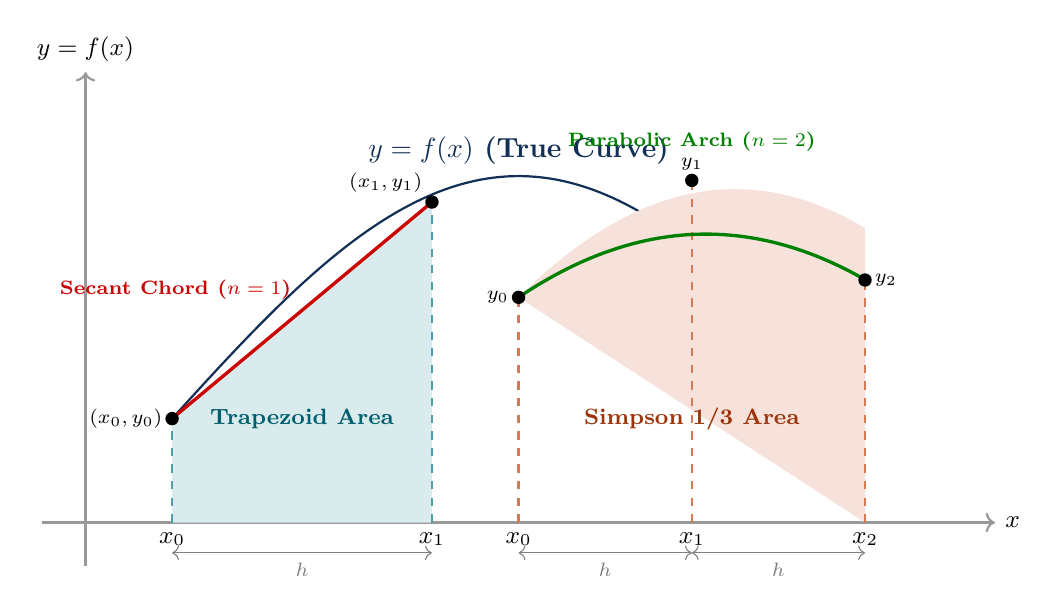
\begin{tikzpicture}[scale=1.1]
    % Axes
    \draw[->, thick, gray!80] (-0.5,0) -- (10.5,0) node[right, black] {\small $x$};
    \draw[->, thick, gray!80] (0,-0.5) -- (0,5.2) node[above, black] {\small $y = f(x)$};
    
    % True curve f(x)
    \draw[thick, primary, domain=1:9, samples=100] plot (\x, {1.2 + 2.8*sin((\x - 1)*22.5)});
    \node[primary, font=\bfseries] at (5.0, 4.3) {$y = f(x)$ (True Curve)};
    
    % Left panel: Trapezoidal Rule (Straight chord)
    \fill[secondary!15] (1,0) -- (1,1.2) -- (4,3.7) -- (4,0) -- cycle;
    \draw[dashed, secondary!70, thick] (1,0) -- (1,1.2);
    \draw[dashed, secondary!70, thick] (4,0) -- (4,3.7);
    \draw[very thick, red!80!black] (1,1.2) -- (4,3.7) node[midway, above left, font=\scriptsize\bfseries, color=red!80!black] {Secant Chord ($n=1$)};
    
    \node[below, font=\small] at (1,0) {$x_0$};
    \node[below, font=\small] at (4,0) {$x_1$};
    \fill[black] (1,1.2) circle (2.2pt) node[left, font=\scriptsize] {$(x_0, y_0)$};
    \fill[black] (4,3.7) circle (2.2pt) node[above left, font=\scriptsize] {$(x_1, y_1)$};
    \node[font=\footnotesize\bfseries, color=secondary!80!black] at (2.5, 1.2) {Trapezoid Area};
    \draw[<->, gray] (1,-0.35) -- (4,-0.35) node[midway, below, font=\scriptsize] {$h$};

    % Right panel: Simpson's 1/3 Rule (Parabola across 3 points)
    \fill[accent!15] (5,0) -- (5,2.6) plot[domain=5:9] (\x, {2.6 + 0.6*(\x-5) - 0.2*(\x-5)*(\x-7)}) -- (9,0) -- cycle;
    \draw[dashed, accent!70, thick] (5,0) -- (5,2.6);
    \draw[dashed, accent!70, thick] (7,0) -- (7,3.95);
    \draw[dashed, accent!70, thick] (9,0) -- (9,2.8);
    
    \draw[very thick, green!50!black, domain=5:9, samples=50] plot (\x, {2.6 + 0.675*(\x-5) - 0.156*(\x-5)*(\x-5)});
    \node[green!50!black, font=\scriptsize\bfseries] at (7.0, 4.4) {Parabolic Arch ($n=2$)};
    
    \node[below, font=\small] at (5,0) {$x_0$};
    \node[below, font=\small] at (7,0) {$x_1$};
    \node[below, font=\small] at (9,0) {$x_2$};
    \fill[black] (5,2.6) circle (2.2pt) node[left, font=\scriptsize] {$y_0$};
    \fill[black] (7,3.95) circle (2.2pt) node[above, font=\scriptsize] {$y_1$};
    \fill[black] (9,2.8) circle (2.2pt) node[right, font=\scriptsize] {$y_2$};
    \node[font=\footnotesize\bfseries, color=accent!80!black] at (7.0, 1.2) {Simpson 1/3 Area};
    \draw[<->, gray] (5,-0.35) -- (7,-0.35) node[midway, below, font=\scriptsize] {$h$};
    \draw[<->, gray] (7,-0.35) -- (9,-0.35) node[midway, below, font=\scriptsize] {$h$};
\end{tikzpicture}
\caption{Geometric comparison between the Trapezoidal rule (linear chord approximation over width $h$) and Simpson's 1/3 rule (quadratic parabolic approximation over double width $2h$).}
\label{fig:quadrature_comparison}
\end{figure}

% =========================================================================
% SUMMARY TABLE OF NEWTON-COTES RULES
% =========================================================================
\section{Comprehensive Summary of Newton--Cotes Quadrature Formulas}
\label{sec:summary_quadrature_table}

\begin{table}[htbp]
\centering
\small
\renewcommand{\arraystretch}{1.4}
\begin{tabular}{|l|c|l|c|c|}
\hline
\textbf{Method} & \textbf{Subintervals $n$} & \textbf{Formula $\int_{x_0}^{x_n} y \, dx$} & \textbf{Degree} & \textbf{Global Error} \\ \hline\hline
\textbf{Trapezoidal} & Any $n \ge 1$ & $\frac{h}{2}[(y_0 + y_n) + 2\sum_{i=1}^{n-1} y_i]$ & 1 & $-\frac{(b-a)h^2}{12} f''(\xi)$ \\ \hline
\textbf{Simpson's 1/3} & Even $n$ & $\frac{h}{3}[(y_0 + y_n) + 4\sum y_{\text{odd}} + 2\sum y_{\text{even}}]$ & 3 & $-\frac{(b-a)h^4}{180} f^{(4)}(\xi)$ \\ \hline
\textbf{Simpson's 3/8} & Multiple of 3 & $\frac{3h}{8}[(y_0 + y_n) + 3\sum y_{\text{rem}} + 2\sum y_{\text{mult 3}}]$ & 3 & $-\frac{3(b-a)h^4}{80} f^{(4)}(\xi)$ \\ \hline
\textbf{Weddle's Rule} & Multiple of 6 & $\frac{3h}{10}[y_0 + 5y_1 + y_2 + 6y_3 + y_4 + 5y_5 + y_6]$ & 5 & $-\frac{(b-a)h^6}{140} f^{(6)}(\xi)$ \\ \hline
\end{tabular}
\caption{Classification, required partition constraints, and truncation errors for Newton--Cotes quadrature rules.}
\end{table}

% =========================================================================
% WORKED EXAMPLES
% =========================================================================
\section{Exhaustive Step-by-Step Solved Examination Problems}
\label{sec:quadrature_solved_problems}

\begin{examplebox}[Standard University Benchmark: Evaluation of $\int_{0}^{6} \frac{dx}{1 + x^2}$]
Evaluate the definite integral:
\begin{equation}
    I = \int_{0}^{6} \frac{1}{1 + x^2} \, dx
\end{equation}
by dividing the interval $[0, 6]$ into $6$ equal subintervals using:
\begin{enumerate}[label=(\roman*),noitemsep]
    \item Trapezoidal Rule
    \item Simpson's 1/3 Rule
    \item Simpson's 3/8 Rule
    \item Weddle's Rule
\end{enumerate}
Compare each result with the exact analytical value:
\begin{equation}
    I_{\text{exact}} = \left[ \arctan(x) \right]_0^6 = \arctan(6) - \arctan(0) \approx 1.40564765 \text{ rad}
\end{equation}

\textbf{Step 1: Construction of the Ordinate Table} \\
With $a = 0, b = 6, n = 6$, the step size is:
\begin{equation}
    h = \frac{b - a}{n} = \frac{6 - 0}{6} = 1
\end{equation}
The nodes and ordinate values $y = f(x) = \frac{1}{1 + x^2}$ to 5 decimal places are:
\begin{center}
\renewcommand{\arraystretch}{1.3}
\begin{tabular}{|c|c|l|l|}
\hline
$i$ & $x_i$ & $y_i = \frac{1}{1 + x_i^2}$ (Fraction) & $y_i$ (Decimal) \\ \hline
0 & 0 & $1 / 1$ & $1.00000$ \\
1 & 1 & $1 / 2$ & $0.50000$ \\
2 & 2 & $1 / 5$ & $0.20000$ \\
3 & 3 & $1 / 10$ & $0.10000$ \\
4 & 4 & $1 / 17$ & $0.05882$ \\
5 & 5 & $1 / 26$ & $0.03846$ \\
6 & 6 & $1 / 37$ & $0.02703$ \\ \hline
\end{tabular}
\end{center}
\end{examplebox}

\subsubsection*{(i) Solution by Trapezoidal Rule}
\begin{align}
    I_T &= \frac{h}{2} \left[ (y_0 + y_6) + 2(y_1 + y_2 + y_3 + y_4 + y_5) \right] \nonumber \\
    &= \frac{1}{2} \left[ (1.00000 + 0.02703) + 2(0.50000 + 0.20000 + 0.10000 + 0.05882 + 0.03846) \right] \nonumber \\
    &= \frac{1}{2} \left[ 1.02703 + 2(0.89728) \right] = \frac{1}{2} \left[ 1.02703 + 1.79456 \right] = \frac{2.82159}{2} = \boxed{1.41080}
\end{align}
Absolute error: $|1.41080 - 1.40565| = 0.00515$.

\subsubsection*{(ii) Solution by Simpson's 1/3 Rule}
Since $n = 6$ is even:
\begin{align}
    I_{S1/3} &= \frac{h}{3} \left[ (y_0 + y_6) + 4(y_1 + y_3 + y_5) + 2(y_2 + y_4) \right] \nonumber \\
    &= \frac{1}{3} \left[ (1.00000 + 0.02703) + 4(0.50000 + 0.10000 + 0.03846) + 2(0.20000 + 0.05882) \right] \nonumber \\
    &= \frac{1}{3} \left[ 1.02703 + 4(0.63846) + 2(0.25882) \right] \nonumber \\
    &= \frac{1}{3} \left[ 1.02703 + 2.55384 + 0.51764 \right] = \frac{4.09851}{3} = \boxed{1.36617}
\end{align}

\subsubsection*{(iii) Solution by Simpson's 3/8 Rule}
Since $n = 6$ is a multiple of 3:
\begin{align}
    I_{S3/8} &= \frac{3h}{8} \left[ (y_0 + y_6) + 3(y_1 + y_2 + y_4 + y_5) + 2(y_3) \right] \nonumber \\
    &= \frac{3(1)}{8} \left[ (1.00000 + 0.02703) + 3(0.50000 + 0.20000 + 0.05882 + 0.03846) + 2(0.10000) \right] \nonumber \\
    &= \frac{3}{8} \left[ 1.02703 + 3(0.79728) + 0.20000 \right] \nonumber \\
    &= \frac{3}{8} \left[ 1.02703 + 2.39184 + 0.20000 \right] = \frac{3}{8} [3.61887] = \boxed{1.35708}
\end{align}

\subsubsection*{(iv) Solution by Weddle's Rule}
Since $n = 6$:
\begin{align}
    I_W &= \frac{3h}{10} \left[ y_0 + 5y_1 + y_2 + 6y_3 + y_4 + 5y_5 + y_6 \right] \nonumber \\
    &= \frac{3(1)}{10} \left[ 1.00000 + 5(0.50000) + 0.20000 + 6(0.10000) + 0.05882 + 5(0.03846) + 0.02703 \right] \nonumber \\
    &= \frac{3}{10} \left[ 1.00000 + 2.50000 + 0.20000 + 0.60000 + 0.05882 + 0.19230 + 0.02703 \right] \nonumber \\
    &= \frac{3}{10} [4.57815] = \boxed{1.37345}
\end{align}

\begin{examplebox}[Approximation of $\pi$ via $\int_{0}^{1} \frac{dx}{1 + x^2}$]
Calculate an approximation of $\pi$ using Simpson's 1/3 rule with $h = 0.25$ ($n = 4$) for the integral:
\begin{equation}
    I = \int_{0}^{1} \frac{1}{1 + x^2} \, dx = \left[ \arctan(x) \right]_0^1 = \frac{\pi}{4} \implies \pi = 4 I
\end{equation}

\textbf{Step 1: Partition and Table of Ordinates} \\
Here $a = 0, b = 1, h = 0.25$, so the nodes are $x_0 = 0, x_1 = 0.25, x_2 = 0.5, x_3 = 0.75, x_4 = 1.0$:
\begin{center}
\renewcommand{\arraystretch}{1.3}
\begin{tabular}{|c|c|l|l|}
\hline
$i$ & $x_i$ & $y_i = \frac{1}{1 + x_i^2}$ & Decimal Value \\ \hline
0 & 0.00 & $1 / (1 + 0) = 1$ & $1.000000$ \\
1 & 0.25 & $1 / (1 + 0.0625) = 16/17$ & $0.941176$ \\
2 & 0.50 & $1 / (1 + 0.25) = 4/5$ & $0.800000$ \\
3 & 0.75 & $1 / (1 + 0.5625) = 16/25$ & $0.640000$ \\
4 & 1.00 & $1 / (1 + 1) = 1/2$ & $0.500000$ \\ \hline
\end{tabular}
\end{center}

\textbf{Step 2: Apply Simpson's 1/3 Rule}
\begin{align}
    I &\approx \frac{h}{3} \left[ (y_0 + y_4) + 4(y_1 + y_3) + 2(y_2) \right] \nonumber \\
    &= \frac{0.25}{3} \left[ (1.000000 + 0.500000) + 4(0.941176 + 0.640000) + 2(0.800000) \right] \nonumber \\
    &= \frac{0.25}{3} \left[ 1.500000 + 4(1.581176) + 1.600000 \right] \nonumber \\
    &= \frac{0.25}{3} \left[ 1.500000 + 6.324704 + 1.600000 \right] = \frac{0.25}{3} [9.424704] = 0.785392
\end{align}

\textbf{Step 3: Compute $\pi$}
\begin{equation}
    \pi \approx 4 \times 0.785392 = \boxed{3.141568}
\end{equation}
Compared to the true value $\pi = 3.14159265\dots$, the numerical approximation is accurate to \textbf{4 decimal places} with only 4 subintervals!
\end{examplebox}


% --- Appendix: Master Formula Cheat Sheet ---
\appendix
\chapter{Master Formula Cheat Sheet and Exam Quick Reference}
\label{ch:cheat_sheet}

\noindent This appendix compiles the complete mathematical toolkit of \textbf{Numerical Analysis} into a dense, high-yield reference guide. All master formulas, convergence rates, error bounds, algorithmic criteria, and operational identities are organized systematically for rapid pre-examination revision and professional numerical computation.

% =========================================================================
% PART I: ROOT-FINDING ALGORITHMS
% =========================================================================
\section{Part I: Nonlinear Equations and Root-Finding Methods}

\begin{conceptbox}[Comparative Summary of Root-Finding Methods]
\small
\renewcommand{\arraystretch}{1.35}
\resizebox{\linewidth}{!}{%
\begin{tabular}{|l|c|c|c|l|}
\hline
\textbf{Method} & \textbf{Iteration Formula} & \textbf{Order $p$} & \textbf{Bracket?} & \textbf{Convergence Criteria / Notes} \\ \hline\hline
\textbf{Bisection} & $x_{m} = \frac{a_k + b_k}{2}$ & $1$ & Yes & Guaranteed if $f(a)f(b) < 0$; $e_{n} \le \frac{b-a}{2^n}$ \\ \hline
\textbf{Regula-Falsi} & $x = \frac{a f(b) - b f(a)}{f(b) - f(a)}$ & $1$ & Yes & Guaranteed bracketing; one endpoint stays fixed \\ \hline
\textbf{Secant} & $x_{k+1} = x_k - f(x_k)\frac{x_k - x_{k-1}}{f(x_k) - f(x_{k-1})}$ & $\frac{1+\sqrt{5}}{2} \approx 1.618$ & No & 1 function call/step; superlinear convergence \\ \hline
\textbf{Newton--Raphson} & $x_{k+1} = x_k - \frac{f(x_k)}{f'(x_k)}$ & $2$ & No & Local quadratic convergence; fails if $f'(x_k) \approx 0$ \\ \hline
\textbf{Fixed-Point} & $x_{k+1} = \phi(x_k)$ & $1$ & No & Converges if $|\phi'(x)| \le k < 1$ in neighborhood \\ \hline
\end{tabular}%
}
\end{conceptbox}

\begin{theorembox}[Newton--Raphson Special Recurrence Formulas]
\begin{enumerate}[label=\textbf{\arabic*.},noitemsep]
    \item \textbf{Division-Free Reciprocal Algorithm ($1/N$):} Solving $f(x) = \frac{1}{x} - N = 0$:
    \begin{equation}
        \boxed{x_{k+1} = x_k (2 - N x_k)} \quad \text{Convergence condition: } 0 < x_0 < \frac{2}{N}
    \end{equation}
    \item \textbf{Square Root Algorithm ($\sqrt{N}$):} Solving $f(x) = x^2 - N = 0$:
    \begin{equation}
        \boxed{x_{k+1} = \frac{1}{2}\left( x_k + \frac{N}{x_k} \right)}
    \end{equation}
    \item \textbf{$p$-th Root Algorithm ($N^{1/p}$):} Solving $f(x) = x^p - N = 0$:
    \begin{equation}
        \boxed{x_{k+1} = \frac{1}{p}\left[ (p - 1)x_k + \frac{N}{x_k^{p-1}} \right]}
    \end{equation}
    \item \textbf{Asymptotic Error Constant:}
    \begin{equation}
        e_{k+1} \approx c \, e_k^2, \quad \text{where } \boxed{c = \frac{f''(\alpha)}{2 f'(\alpha)}}
    \end{equation}
\end{enumerate}
\end{theorembox}

\begin{notebox}[Birge--Vieta Method (Double Synthetic Division for Polynomials)]
To find a root of $P_n(x) = a_0 x^n + a_1 x^{n-1} + \dots + a_n$ near $p$:
\begin{align}
    b_0 &= a_0, \qquad b_k = a_k + p\,b_{k-1} \quad (k = 1, \dots, n) \implies P(p) = b_n \\
    c_0 &= b_0, \qquad c_k = b_k + p\,c_{k-1} \quad (k = 1, \dots, n-1) \implies P'(p) = c_{n-1}
\end{align}
\begin{equation}
    \boxed{p_{\text{new}} = p - \frac{b_n}{c_{n-1}}}
\end{equation}
\end{notebox}

% =========================================================================
% PART II: LINEAR SYSTEMS OF EQUATIONS
% =========================================================================
\section{Part II: Direct and Iterative Linear Solvers}

\begin{theorembox}[Direct Solvers: Gauss Elimination and Gauss--Jordan]
\textbf{Gauss Elimination (Triangularization):}
\begin{equation}
    m_{ik} = \frac{a_{ik}^{(k-1)}}{a_{kk}^{(k-1)}} \quad (i = k+1, \dots, n), \qquad a_{ij}^{(k)} = a_{ij}^{(k-1)} - m_{ik} a_{kj}^{(k-1)}
\end{equation}
Backward substitution: $x_n = \frac{b_n^{(n)}}{a_{nn}^{(n)}}$, $x_i = \frac{1}{a_{ii}^{(i)}} \left( b_i^{(i)} - \sum_{j=i+1}^n a_{ij}^{(i)} x_j \right)$.

\textbf{Partial Pivoting Strategy:} At stage $k$, find row $p \ge k$ such that $|a_{pk}| = \max_{k \le i \le n} |a_{ik}|$, and interchange row $k \leftrightarrow$ row $p$. Prevents numerical instability and blowup from near-zero pivots.
\end{theorembox}

\begin{theorembox}[Iterative Solvers: Jacobi vs. Gauss--Seidel]
Decompose matrix $A = L + D + U$ into strictly lower, diagonal, and strictly upper parts.
\begin{itemize}[noitemsep]
    \item \textbf{Jacobi Method (Simultaneous Displacements):}
    \begin{align}
        \text{Component form: } \quad & \boxed{x_i^{(k+1)} = \frac{1}{a_{ii}} \left( b_i - \sum_{j \ne i} a_{ij} x_j^{(k)} \right)} \\
        \text{Matrix form: } \quad & \boxed{x^{(k+1)} = -D^{-1}(L + U) x^{(k)} + D^{-1} b}
    \end{align}
    \item \textbf{Gauss--Seidel Method (Successive Displacements):}
    \begin{align}
        \text{Component form: } \quad & \boxed{x_i^{(k+1)} = \frac{1}{a_{ii}} \left( b_i - \sum_{j < i} a_{ij} x_j^{(k+1)} - \sum_{j > i} a_{ij} x_j^{(k)} \right)} \\
        \text{Matrix form: } \quad & \boxed{x^{(k+1)} = -(D+L)^{-1} U x^{(k)} + (D+L)^{-1} b}
    \end{align}
    \item \textbf{Sufficient Condition for Convergence:} $A$ is \textbf{strictly diagonally dominant}:
    \begin{equation}
        \boxed{|a_{ii}| > \sum_{j \ne i} |a_{ij}| \quad \forall i = 1, 2, \dots, n}
    \end{equation}
    \item Spectral radius criterion: $\rho(M) < 1$, where $M$ is the respective iteration matrix.
\end{itemize}
\end{theorembox}

% =========================================================================
% PART III: EIGENVALUES AND MATRIX BOUNDS
% =========================================================================
\section{Part III: Matrix Eigenvalues and Spectral Bounds}

\begin{theorembox}[Gerschgorin's Circle Theorem and Disc Formulas]
Let $A \in \mathbb{C}^{n \times n}$.
\begin{enumerate}[label=\textbf{\arabic*.},noitemsep]
    \item \textbf{Row Gerschgorin Discs:} Every eigenvalue $\lambda$ of $A$ lies in the union:
    \begin{equation}
        \boxed{\lambda \in \bigcup_{i=1}^n D_i, \quad D_i = \left\{ z \in \mathbb{C} : |z - a_{ii}| \le R_i \right\}, \quad R_i = \sum_{j \ne i} |a_{ij}|}
    \end{equation}
    \item \textbf{Column Gerschgorin Discs:} Since eigenvalues of $A^T$ are identical to $A$:
    \begin{equation}
        \boxed{\lambda \in \bigcup_{j=1}^n C_j, \quad C_j = \left\{ z \in \mathbb{C} : |z - a_{jj}| \le K_j \right\}, \quad K_j = \sum_{i \ne j} |a_{ij}|}
    \end{equation}
    \item \textbf{Optimal Bound:} $\lambda \in \left( \bigcup_{i=1}^n D_i \right) \cap \left( \bigcup_{j=1}^n C_j \right)$.
    \item \textbf{Disjoint Subsets:} If a union of $k$ discs is disjoint from the remaining $n - k$ discs, it contains exactly $k$ eigenvalues (counting algebraic multiplicities).
\end{enumerate}
\end{theorembox}

\begin{notebox}[Power Method for Dominant Eigenpair]
Given matrix $A$ with dominant eigenvalue $|\lambda_1| > |\lambda_2| \ge \dots \ge |\lambda_n|$:
\begin{equation}
    y^{(k+1)} = A x^{(k)}, \qquad m_{k+1} = \max_i |y_i^{(k+1)}|, \qquad x^{(k+1)} = \frac{y^{(k+1)}}{m_{k+1}}
\end{equation}
As $k \to \infty$: $\boxed{\lambda_1 \approx m_k}, \quad \boxed{v_1 \approx x^{(k)}}$. \\
Rayleigh Quotient estimate: $\lambda_1 \approx \frac{(x^{(k)})^T A x^{(k)}}{(x^{(k)})^T x^{(k)}}$.
\end{notebox}

% =========================================================================
% PART IV: FINITE DIFFERENCES AND OPERATOR ALGEBRA
% =========================================================================
\section{Part IV: Finite Differences and Operator Algebra}

\begin{conceptbox}[Fundamental Operator Definitions]
Let $y_x = f(x)$ with uniform grid spacing $h$:
\begin{align}
    \textbf{Forward Difference:} \quad &\Delta f(x) = f(x+h) - f(x) = (E - 1) f(x) \\
    \textbf{Backward Difference:} \quad &\nabla f(x) = f(x) - f(x-h) = (1 - E^{-1}) f(x) \\
    \textbf{Shift Operator:} \quad &E f(x) = f(x+h) = e^{h D} f(x) \\
    \textbf{Central Difference:} \quad &\delta f(x) = f\left(x + \frac{h}{2}\right) - f\left(x - \frac{h}{2}\right) = (E^{1/2} - E^{-1/2}) f(x) \\
    \textbf{Averaging Operator:} \quad &\mu f(x) = \frac{1}{2}\left[ f\left(x + \frac{h}{2}\right) + f\left(x - \frac{h}{2}\right) \right] = \frac{1}{2}(E^{1/2} + E^{-1/2}) f(x) \\
    \textbf{Differential Operator:} \quad &D f(x) = \frac{df}{dx}
\end{align}
\end{conceptbox}

\begin{theorembox}[Master Operational Identities]
\begin{minipage}{0.48\textwidth}
\begin{itemize}[noitemsep]
    \item $E = 1 + \Delta = (1 - \nabla)^{-1} = e^{hD}$
    \item $\nabla = 1 - E^{-1} = \Delta E^{-1} = 1 - (1+\Delta)^{-1}$
    \item $\delta = E^{1/2} - E^{-1/2} = \Delta E^{-1/2} = \nabla E^{1/2}$
    \item $\Delta \nabla = \nabla \Delta = \Delta - \nabla = \delta^2$
\end{itemize}
\end{minipage}
\hfill
\begin{minipage}{0.48\textwidth}
\begin{itemize}[noitemsep]
    \item $\mu = \frac{1}{2}(E^{1/2} + E^{-1/2}) = \sqrt{1 + \frac{1}{4}\delta^2}$
    \item $\mu^2 = 1 + \frac{1}{4}\delta^2 \iff 4\mu^2 - \delta^2 = 4$
    \item $\mu \delta = \frac{1}{2}(\Delta + \nabla)$
    \item $h D = \ln(1 + \Delta) = -\ln(1 - \nabla) = \sinh^{-1}(\delta)$
\end{itemize}
\end{minipage}
\end{theorembox}

\begin{theorembox}[Factorial Polynomials and Series Summation]
\begin{enumerate}[label=\textbf{\arabic*.},noitemsep]
    \item \textbf{Definition:} $x^{(n)} = x(x-h)(x-2h)\dots(x-(n-1)h)$ (for $h = 1$: $x^{(n)} = x(x-1)\dots(x-n+1)$).
    \item \textbf{Finite Difference Derivative Rule:}
    \begin{equation}
        \boxed{\Delta x^{(n)} = n h \, x^{(n-1)}} \qquad (\text{For } h = 1: \Delta x^{(n)} = n x^{(n-1)})
    \end{equation}
    \item \textbf{Fundamental Theorem of Finite Differences:} For any polynomial $P_n(x)$ of degree $n$:
    \begin{equation}
        \boxed{\Delta^n P_n(x) = a_0 \, n! \, h^n = \text{Constant}}, \qquad \boxed{\Delta^{n+k} P_n(x) = 0 \quad (\forall k \ge 1)}
    \end{equation}
    \item \textbf{Summation of Finite Series via Anti-Difference $\Delta^{-1}$:}
    \begin{equation}
        \boxed{\sum_{x=a}^{b-1} f(x) = \left[ \Delta^{-1} f(x) \right]_{a}^{b}} \quad \text{where } \Delta^{-1} x^{(n)} = \frac{x^{(n+1)}}{n+1} + C
    \end{equation}
\end{enumerate}
\end{theorembox}

% =========================================================================
% PART V: INTERPOLATION AND NUMERICAL DIFFERENTIATION
% =========================================================================
\section{Part V: Interpolation Formulas and Numerical Differentiation}

\begin{theorembox}[Equal Spacing Interpolation Formulas]
Let $x_i = x_0 + i h$.
\begin{enumerate}[label=\textbf{\arabic*.},noitemsep]
    \item \textbf{Newton's Forward Formula (Near Beginning of Table):} $p = \frac{x - x_0}{h}$:
    \begin{equation}
        \boxed{P_n(x) = y_0 + p \Delta y_0 + \frac{p(p-1)}{2!} \Delta^2 y_0 + \dots + \frac{p(p-1)\dots(p-n+1)}{n!} \Delta^n y_0}
    \end{equation}
    Error: $R_n(x) = \frac{p(p-1)\dots(p-n)}{(n+1)!} h^{n+1} f^{(n+1)}(\xi)$.
    \item \textbf{Newton's Backward Formula (Near End of Table):} $p = \frac{x - x_n}{h}$:
    \begin{equation}
        \boxed{P_n(x) = y_n + p \nabla y_n + \frac{p(p+1)}{2!} \nabla^2 y_n + \dots + \frac{p(p+1)\dots(p+n-1)}{n!} \nabla^n y_n}
    \end{equation}
    Error: $R_n(x) = \frac{p(p+1)\dots(p+n)}{(n+1)!} h^{n+1} f^{(n+1)}(\xi)$.
\end{enumerate}
\end{theorembox}

\begin{theorembox}[Unequal Spacing Interpolation Formulas]
Given arbitrary distinct nodes $x_0, x_1, \dots, x_n$:
\begin{enumerate}[label=\textbf{\arabic*.},noitemsep]
    \item \textbf{Lagrange's Interpolation Formula:}
    \begin{equation}
        \boxed{P_n(x) = \sum_{i=0}^n y_i L_i(x)}, \qquad \boxed{L_i(x) = \prod_{j \ne i} \frac{x - x_j}{x_i - x_j}}
    \end{equation}
    Cardinal property: $L_i(x_j) = \delta_{ij}$, $\sum_{i=0}^n L_i(x) \equiv 1$.
    \item \textbf{Newton's Divided Difference Formula:}
    \begin{equation}
        \boxed{P_n(x) = f[x_0] + (x - x_0) f[x_0, x_1] + (x - x_0)(x - x_1) f[x_0, x_1, x_2] + \dots}
    \end{equation}
    Divided difference relation to ordinary difference: $f[x_0, x_1, \dots, x_n] = \frac{\Delta^n y_0}{n! h^n} = \frac{f^{(n)}(\xi)}{n!}$.
\end{enumerate}
\end{theorembox}

\begin{theorembox}[Numerical Differentiation Formulas at Tabular Grid Nodes]
From $h D = \ln(1 + \Delta) = \Delta - \frac{\Delta^2}{2} + \frac{\Delta^3}{3} - \frac{\Delta^4}{4} + \dots$:
\begin{align}
    \boxed{\left. \frac{dy}{dx} \right|_{x=x_0} = \frac{1}{h} \left[ \Delta y_0 - \frac{1}{2} \Delta^2 y_0 + \frac{1}{3} \Delta^3 y_0 - \frac{1}{4} \Delta^4 y_0 + \dots \right]} \\
    \boxed{\left. \frac{d^2 y}{dx^2} \right|_{x=x_0} = \frac{1}{h^2} \left[ \Delta^2 y_0 - \Delta^3 y_0 + \frac{11}{12} \Delta^4 y_0 - \frac{5}{6} \Delta^5 y_0 + \dots \right]}
\end{align}
At backward endpoint $x = x_n$ (using $\nabla$):
\begin{align}
    \boxed{\left. \frac{dy}{dx} \right|_{x=x_n} = \frac{1}{h} \left[ \nabla y_n + \frac{1}{2} \nabla^2 y_n + \frac{1}{3} \nabla^3 y_n + \frac{1}{4} \nabla^4 y_n + \dots \right]} \\
    \boxed{\left. \frac{d^2 y}{dx^2} \right|_{x=x_n} = \frac{1}{h^2} \left[ \nabla^2 y_n + \nabla^3 y_n + \frac{11}{12} \nabla^4 y_n + \frac{5}{6} \nabla^5 y_n + \dots \right]}
\end{align}
\end{theorembox}

% =========================================================================
% PART VI: NUMERICAL QUADRATURE
% =========================================================================
\section{Part VI: Numerical Quadrature and Newton--Cotes Rules}

\begin{theorembox}[General Quadrature Formula (Page 68)]
\begin{equation}
    \boxed{
    \int_{x_0}^{x_0 + n h} y \, dx = n h \left[ y_0 + \frac{n}{2} \Delta y_0 + \frac{n(2n-3)}{12} \Delta^2 y_0 + \frac{n(n-2)^2}{24} \Delta^3 y_0 + \dots \right]
    }
\end{equation}
\end{theorembox}

\begin{conceptbox}[Master Newton--Cotes Quadrature Quick Reference Table]
\small
\renewcommand{\arraystretch}{1.45}
\resizebox{\linewidth}{!}{%
\begin{tabular}{|l|c|l|c|c|}
\hline
\textbf{Quadrature Rule} & \textbf{Nodes $n$} & \textbf{Evaluation Formula $\int_{x_0}^{x_n} y \, dx$} & \textbf{Exact Degree} & \textbf{Global Error} \\ \hline\hline
\textbf{Trapezoidal Rule} & Any $n \ge 1$ & $\frac{h}{2} \left[ (y_0 + y_n) + 2 \sum_{i=1}^{n-1} y_i \right]$ & $1$ & $-\frac{(b-a)h^2}{12} f''(\xi)$ \\ \hline
\textbf{Simpson's 1/3 Rule} & Even $n$ & $\frac{h}{3} \left[ (y_0 + y_n) + 4 \sum y_{\text{odd}} + 2 \sum y_{\text{even}} \right]$ & $3$ & $-\frac{(b-a)h^4}{180} f^{(4)}(\xi)$ \\ \hline
\textbf{Simpson's 3/8 Rule} & Mult of 3 & $\frac{3h}{8} \left[ (y_0 + y_n) + 3 \sum y_{\text{rem}} + 2 \sum y_{\text{mult 3}} \right]$ & $3$ & $-\frac{3(b-a)h^4}{80} f^{(4)}(\xi)$ \\ \hline
\textbf{Weddle's Rule} & Mult of 6 & $\frac{3h}{10} \left[ y_0 + 5y_1 + y_2 + 6y_3 + y_4 + 5y_5 + y_6 \right]$ & $5$ & $-\frac{(b-a)h^6}{140} f^{(6)}(\xi)$ \\ \hline
\end{tabular}%
}
\end{conceptbox}

\vspace{0.5cm}
\begin{center}
\small
\textit{Compiled for students and researchers by \href{https://sciqb.com}{\color{secondary}\textbf{sciqb}} --- Academic Session 2026.}
\end{center}


\end{document}
